\documentclass[10pt,a4paper]{book}
\usepackage[utf8]{inputenc}
\usepackage[francais]{babel}
\frenchbsetup{StandardLists=true}
\usepackage{enumitem}
\usepackage[T1]{fontenc}
\usepackage{amsmath}
\usepackage{amsfonts}
\usepackage{amssymb}
\usepackage{graphicx}
\usepackage[counterclockwise]{rotating}
\usepackage{multirow}
\usepackage[usenames, dvipsnames]{xcolor}
\usepackage{tikz}
\usepackage[left=2cm,right=2cm,top=2.5cm,bottom=2.5cm]{geometry}
\usepackage{amsthm}
\usepackage{siunitx}
\usepackage[ruled]{algorithm}
\usepackage{algpseudocode}
\alglanguage{pseudocode}

\newtheorem{definition}{D\'efinition}
\newtheorem{exemple}{Exemple}
\newtheorem{remarque}{Remarque}
\newtheorem{proposition}{Proposition}
\newtheorem{theoreme}[proposition]{Théorème}
\newtheorem{lemme}[proposition]{Lemme}
\newtheorem{corollaire}[proposition]{Corollaire}

\def\gint{\displaystyle\int}
\def\gsum{\displaystyle\sum\limits}
\def\longarc{\text{longarc}}
\def\rang{\text{rang}}
\def\REF{\textbf{REF} }
\def\vort{\text{vort}}
\def\rot{\text{rot}}
\def\Sp{\text{Sp}}
\def\dec{\text{déc}}
\def\vec{\text{vec}}
\def\Vect{\text{Vect}}

\author{Brachet Matthieu}
\title{Schémas compacts hermitiens sur la Sphère - applications en climatologie et océanographie numérique}

\graphicspath{{./Images/}}
\begin{document}
\maketitle
\tableofcontents
\listoffigures
\listoftables

%\section*{Introduction}
%%%% *** INTRODUCTION ***************************************************************************

\section{Introduction}
\label{sec:1}
In this paper, we continue the development
of the compact scheme approach introduced in \cite{} and \cite{}
for hyperbolic problems on the sphere.
In recent years a lot of effort
has been devoted to import
ideas of numerical gas dynamics to numerical climatology.
Two particular examples are finite volumes upwind schemes 
with numerical fluxes. This approach involves
reconstruction with piecewise cubic recontsruction.
A variant is the Discontinuous Galerkin approach
in which several unknowns in a single computational cells are used.
In each of these two cases, the machinery of upwind schemes is adapted
to the specificity of the spherical context
and of the test cases. This involves in particular 
slope limiting. 

An important challenge for numerical schemes in numerical climatology 
is to calculate as accurately as possible 
the solution of linear equations up to a large physical time.
Here we show that our compact scheme performs well
for the three following problems:
\begin{itemize}
\item 
The linear scalar equation
advection 
\begin{equation}
\label{eq:adv}
\dfrac{\partial h}{\partial t}  (t,\mathbf{x})+ \mathbf{c}(t,\mathbf{x}) \cdot \nabla_T h(t,\mathbf{x})=0
\end{equation}

The velocity $\mathbf{c}(t,\mathbf{x}) \in (0, +\infty) \times \mathbb{S}^2$ is prescribed
so that the scalar value $h(t,\mathbf{x})$ exhibits a moving rollup vortex.
This test case was introduced
in \cite{Nair-Machenhauer,Nair-Jablonowski}. We refer to Sections
\ref{sec:4.1} and \ref{sec:4.2} for setails.
\item
The linearized shallow water equations (LSWE). This equation
is expressed as:
\begin{equation}
\label{eq:lswe}
(LSWE) \left\{
\begin{array}{l}
\dfrac{\partial \mathbf{v} }{\partial t} (t,\mathbf{x})+ g \nabla_T \eta(t,\mathbf{x}) + f(\mathbf{x}) \mathbf{k}(\mathbf{x}) \wedge
\mathbf{v}(t,\mathbf{x})=0\\
\dfrac{\partial \eta}{\partial t} (t,\mathbf{x})+ H \nabla_T \cdot \mathbf{v}(t,\mathbf{x})=0
\end{array}
\right.
\end{equation}


This system serves as a base for spherical waves on the sphere,
\cite{Paldor}. The state at rest is 
$(\mathbf{v}_0,\eta_0)=(0,H)$ and the 
The 3-components perturbation unknowns is
the vector $(t,\mathbf{x}) \mapsto (\mathbf{v}(t,\mathbf{x}), \eta(t,\mathbf{x}))$.
\item The shallow water equation (SWE). We use the vectorial form as following :
\begin{equation}
\label{eq:swe}
(SWE) \left\lbrace
\begin{array}{rcl}
\dfrac{\partial h^{\star}}{\partial t} (t,\mathbf{x}) + \nabla_T \cdot \left( h^{\star}(t,\mathbf{x}) \mathbf{v}(t,\mathbf{x}) \right) & = & 0 \\
\dfrac{\partial \mathbf{v}}{\partial t}  (t,\mathbf{x}) + \nabla_T \left( \dfrac{1}{2} \mathbf{v}(t,\mathbf{x})^2 + g h(t,\mathbf{x}) \right) + \left( f(\mathbf{x}) + \zeta(t,\mathbf{x}) \right) \mathbf{k}(\mathbf{x}) \wedge \mathbf{v}(t,\mathbf{x}) & = & \mathbf{0} 
\end{array}
\right.
\end{equation}

where $\zeta = \left( \nabla_T \wedge \mathbf{v} \right) \cdot \mathbf{k}$ is the relative vorticity. $h^{\star} = h - h_s$ with $h_s$ the reliefs map.
\end{itemize}

The present approach is related to compact scheme
approach. In this sense, it belongs 
to a classical approach, which can
be traced back to early works
in approximation and interpolation theory, \cite{Collatz}.

Two specific applications in CFD where compact schemes
are  is Aeroacoustics, \cite{Visbal-Gaitonde, Tam-Webb} and Turbulence, \cite{Lele, Kim-Moin}.

Finite difference schemes 
for simulating problems in climatology have
actually attracted interest since 
more than 40 years, \cite{Arakawa}.

In both cases, we show 
that our purely Cartesian approach supports
the comparison with modern conservative schemes on unstructured grids, such as 
Discontinuous Galerkin or Finite-Volume schemes.
Note finally that Finite Difference methods were recently used
in numerical climatology in \cite{Ghader-Nordstrom}.

The outline of the paper is as follows.
In Section \ref{sec:2}, we recall the numerical calculation
of the gradient introduced in \cite{Croisille-10}. Then in Section 
\label{sec:3}, we present the numerical scheme with emphasis 
on the role of the filtering. Dissipation and dispersion analysis 
is given. Finally in Section \ref{sec:4}, we present 
numerical results on two vortex advection problems mentionned above.
These results show the accuracy of our scheme.
The accuracy is comparable to conservative schemes such as DG schemes \cite{Nair-Jablonowski}.
%
%\part{Rapport de thèse}
%%% SWE.tex

\chapter{Modèle mathématique}

Le plan de ce chapitre sera probablement largement retouché par la suite.

\section{Cadre du problème}

\begin{itemize}
\item Navier Stokes equation(NSE);
\item faible prodondeur;
\item force de Coriolis
\end{itemize}

\section{Equations Shallow Water}

\subsection{Dérivation des équations Shallow Water (SWE)}

\subsection{Equations Shallow Water linéarisé (LSWE)}

\subsection{Approximations possibles sur la force de Coriolis}

\begin{itemize}
\item Approximation sur la force de Coriolis
\item f-plan
\item $\beta-$plan
\end{itemize}

\subsection{Ondes pour LSWE}

\subsection{Relations de conservations}
\chapter{Schémas aux différences}

\section{Opérateurs aux différences en dimension 1}

\subsection{Notations}
\label{sec:notation_1D}

On considère $\Omega = [a,b]$, $a<b$, un intervalle de $\mathbb{R}$ de longueur $L=b-a$. Nous utilisons les lettres latines pour noter les fonctions continues : $f(x)$, $u(x)$, ... $x \in \Omega$. Pour $u$ et $v$, des fonctions définies sur $\Omega$, le produit scalaire dans $L^2 ( \Omega )$ est défini par
\begin{equation}
(u,v) = \gint_{\Omega} u(x) \bar{v}(x) dx = \gint_{a}^b u(x) \bar{v}(x) dx.
\end{equation}
Pour $u$ et $v$ à valeurs réelles, on a
\begin{equation}
(u,v) = \gint_{a}^b u(x) v(x) dx.
\end{equation}
La norme sur $L^2(\Omega)$ est donnée par :
\begin{equation}
\| u \|_{L^2(\Omega)} = \sqrt{(u,u)}
\end{equation}
Pour $u \in L^{\infty}(\Omega)$, on note
\begin{equation}
\| u \|_{\infty} = \sup_{x\in\Omega} |u(x)|.
\end{equation}
Une fonction $u : x \in \mathbb{R} \mapsto u(x) \in \mathbb{R}$ est \textit{périodique} de période $L$ si 
\begin{equation}
u(x+L) = u(x) \text{, } \forall x \in \mathbb{R}.
\end{equation}
En particulier, on a $u(a)=u(b)$.

On considère une grille régulière sur $\Omega$ constituée de $N \geq 1$ points :
\begin{equation}
a=x_0 < x_1 < \ldots < x_{N-1} < x_N = b,
\end{equation}
où les valeurs $x_i$ sont définies par :
\begin{equation}
x_i = a + ih\text{, } i = 0,1, \ldots,N \text{ et } h = \dfrac{b-a}{N} \text{ le pas d'espace}. 
\end{equation}

\begin{figure}[htbp]
\begin{center}
\begin{tikzpicture}[scale=1.8]
	\draw [>=stealth, <->] (-2,0.2) -- (-1,.2) ;
	\draw (-1.5,.3) node[above] {$h$} ;
	\draw (-3,0) -- (3,0) ;
	\draw (-3,0) node {$\times$} ;
	\draw (-3,-.2) node[below] {$x_0=a$} ;
	\draw (-2,0) node {$\bullet$} ;
	\draw (-2,-.2) node[below] {$x_1$} ;
	\draw (-1,0) node {$\bullet$} ;
	\draw (-1,-.2) node[below] {$x_2$} ;
	\draw (0,-.2) node[below] {$\ldots$} ;
	\draw (1,0) node {$\bullet$} ;
	\draw (1,-.2) node[below] {$x_{N-2}$} ;
	\draw (2,0) node {$\bullet$} ;
	\draw (2,-.2) node[below] {$x_{N-1}$} ;
	\draw (3,0) node {$\times$} ;
	\draw (3,-.2) node[below] {$x_N =b$} ;
\end{tikzpicture}
\end{center}
\caption{Grille en dimension 1. Les symboles $\times$ désignent les points de bords, les symboles $\bullet$ désignent les points intérieurs de la grille.}
\label{fig:maillage1D}
\end{figure}

Les points $x_0=a$ et $x_N = a + L = b$ sont les points de bord du domaine et les points $(x_j)_{1 \leq j \leq N-1}$ désignent les points intérieurs. 

Nous distinguons trois types de données aux points de grille $x_j$, $0 \leq j \leq N$ :
\begin{enumerate}
\item Une \textit{fonction de grille} est une fonction définie uniquement aux points $(x_j)_{0 \leq j \leq N}$. Les fonctions de grilles sont notées en fonte gothique : $\mathfrak{u}$, $\mathfrak{v}$, ... 
On note
\begin{equation}
\mathfrak{u} = (\mathfrak{u}(x_0), \mathfrak{u}(x_1), \mathfrak{u}(x_2), ... , \mathfrak{u}(x_N)).
\end{equation}
De plus, $l^2_h$ désigne l'espace des fonctions de grille, $h>0$ fixé.
On munit cet espace du produit scalaire et de la norme associée :
\begin{equation}
(\mathfrak{u},\mathfrak{v})_h = h \gsum_{j=0}^N \mathfrak{u}(x_j) \mathfrak{v}(x_j) \text{,  } |\mathfrak{u}|_h^2 = h \gsum_{j=0}^N \mathfrak{u}(x_j)^2.
\end{equation}
On définit aussi la norme infinie pour les fonctions de grille :
\begin{equation}
\| \mathfrak{u} \|_{\infty} = \max_{0\leq j \leq N} |\mathfrak{u}(x_j)|.
\end{equation}
On notera 
\begin{equation}
\mathfrak{u}_j = \mathfrak{u}(x_j) \text{ pour tout } 0\leq j \leq N.  
\end{equation}

On note $l^2_{h,per}$ l'espace des fonctions de grilles périodiques. Si $\mathfrak{u} \in l^2_{h,per}$ alors $\mathfrak{u}(x_0) = \mathfrak{u}(x_N)$ et on a
\begin{equation}
\mathfrak{u}=(\mathfrak{u}(x_0), \mathfrak{u}(x_1), ..., \mathfrak{u}(x_{N-1})).
\end{equation}
Le produit scalaire et la norme associée dans $l^2_{h,per}$ sont
\begin{equation}
(\mathfrak{u},\mathfrak{v})_{h,per} = h \gsum_{j=0}^{N-1} \mathfrak{u}(x_j) \bar{\mathfrak{v}}(x_j) \text{,  } |\mathfrak{u}|_h^2 = h \gsum_{j=1}^N |\mathfrak{u}(x_j)|^2 \text{ avec} \mathfrak{u}, \mathfrak{v} \in l^2_{h,per}.
\end{equation}
La norme infinie dans $l^2_{h,per}$ est
\begin{equation}
\| \mathfrak{u} \|_{\infty} = \max_{0\leq j \leq N-1} |\mathfrak{u}(x_j)|.
\end{equation}



\item Les lettres latines capitales désignent les vecteurs de $\mathbb{R}^{N+1}$ et les matrices de $\mathbb{M}_{N+1}(\mathbb{R})$. Par exemple, soit le vecteur $U \in \mathbb{R}^{N+1}$ des composantes de $\mathfrak{u} \in l^2_h$ :
\begin{equation}
U = \begin{bmatrix}
\mathfrak{u}_0 \\ \mathfrak{u}_1 \\ \vdots \\ \mathfrak{u}_N
\end{bmatrix} =
\begin{bmatrix}
\mathfrak{u}(x_0) \\ \mathfrak{u}(x_1) \\ \vdots \\ \mathfrak{u}(x_N)
\end{bmatrix}
\end{equation}
La norme euclidienne sur $\mathbb{R}^{N+1}$ est notée $|U|$. Elle induit une norme pour les matrices $A \in \mathbb{M}_{N+1}(\mathbb{R})$ définie par
\begin{equation}
|A|_2 = \sup_{U \neq 0} \dfrac{|AU|}{|U|}.
\end{equation}
Si $A$ est symétrique alors :
\begin{equation}
|A|_2 = \rho(A) := \max \left\lbrace |\lambda| \text{ tels que } \lambda \in \Sp (A) \right\rbrace.
\end{equation}
$\rho(A)$ est nommé \textit{rayon spectrale} de $A$.
La norme infinie de $U$ est donnée par :
\begin{equation}
|U|_{\infty} = \max_{1 \leq j \leq N+1} |U_j|.
\end{equation}
La norme sur $\mathbb{M}_{N+1}(\mathbb{R})$ subordonnée à $|\cdot|_{\infty}$ est
\begin{equation}
|A|_{\infty} = \sup_{U \neq 0} \dfrac{|AU|_{\infty}}{|U|_{\infty}} = \max_{1 \leq i \leq N+1} \gsum_{j=1}^{N+1} |A_{i,j}|.
\end{equation}



\item Soit $u: x \in \Omega \mapsto u(x)$, on définit la \textit{fonction de grille} $u^*$ associée à $u$ par :
\begin{equation}
u^*_j = u^*(x_j) \text{ pour } 0 \leq j \leq N.
\end{equation}
$u^*$ est donc la restriction de $u$ aux points de la grille. Si $u$ est une fonction périodique, alors $u^*$ est définit par
\begin{equation}
u^*_j = u^*(x_j) \text{ pour } 1 \leq j \leq N.
\end{equation}
\end{enumerate}

Nous distinguons $l^2_h$, l'espace des fonctions de grilles, de $\mathbb{R}^{N+1}$ même si ces deux espaces sont isomorphes.

Cette distinction permet de faire une claire différences entre :
\begin{itemize}
\item les opérateurs aux différences finies, qui agissent sur les fonctions de grilles,
\item les matrices, qui agissent sur les vecteurs.
\end{itemize}
Les fonctions de grilles contiennent toutes les échelles nécessaires dans le contexte physique alors que les vecteurs sont sans dimension. De plus, le raisonnement au niveau discret est plus naturel avec les fonctions de grilles. Il s'effectue d'une façon abstraite à l'aide d'opérateurs aux différences. En revanche, le codage est effectuée dans le cadre de l'algèbre linéaire.

Si $u : x \in \Omega \mapsto u(x) \in \mathbb{R}$est une fonction régulière telle que $u(a) = u(b) = 0$ alors $(\partial_x u)^*$ désigne la restriction à la grille de la fonction $\partial_x u$ associée à la dérivée première de $u$. On peut approcher cette donnée à l'aide de $\mathfrak{u}_x$ obtenue grâce à l'opérateur $\delta_x$ agissant sur les fonctions de grilles et donné par
\begin{equation}
\mathfrak{u}_{x,j} = \delta_x u^*(x_j) = \dfrac{u(x_{j+1}) - u(x_{j-1})}{2h}.
\end{equation}
En effet, par développement de Taylor, on a 
\begin{equation}
u(x_j+h) = u(x_j) + h \partial_x u(x_j) + \dfrac{h^2}{2} \partial_x^2 u(x_j) + \dfrac{h^3}{6} \partial_x^3 u(\xi) \text{ avec } \xi \in [x_j, x_j+h].
\end{equation}
De la même manière, en $x_j-h$, on a 
\begin{equation}
u(x_j-h) = u(x_j) - h \partial_x u(x_j) + \dfrac{h^2}{2} \partial_x^2 u(x_j) - \dfrac{h^3}{6} \partial_x^3 u(\eta) \text{ avec } \eta \in [x_j-h, x_j].
\end{equation}
Soit $0 \leq j \leq N$, alors
\begin{align*}
\delta_x u^*(x_j) & = \dfrac{u(x_{j+1}) - u(x_{j-1})}{2h}\\
                  & = \dfrac{1}{2h} \left[ 2h \partial_x u(x_j) + \dfrac{h^3}{6} \partial_x^3 u(\xi) + \dfrac{h^3}{6} \partial_x^3 u(\eta) \right]\\
                  & = \partial_x u(x_j) + \dfrac{h^2}{2} \left[ \dfrac{1}{6} \partial_x^3 u(\xi) + \dfrac{1}{6} \partial_x^3 u(\eta) \right] \\
                  & = \partial_x u(x_j) + \dfrac{h^2}{6} \partial_x^3 u(\gamma) \text{ avec } \gamma \in ]x_j-h , x_j+h[ \text{ par théorème des valeurs intermédiaires.}
\end{align*}
L'erreur de troncature est une fonction de grille définie en chaque point du $x_j$ par
\begin{align*}
\mathfrak{t}(x_j) & = \delta_x u^*(x_j) - \delta_x u^*(x_j)\\
                  & = \dfrac{h^2}{6} \partial_x^3 u(\gamma) \text{ avec } \gamma \in ]x_j-h , x_j+h[.
\end{align*}




















\subsection{Transformée de Fourier discrète}

Pour simplifier les notations, on considère $a=0$ et $b=L$. Le pas du maillage est $h = \frac{L}{N}$.
Soit, pour tout $k$ vérifiant $-N/2+1 \leq k \leq N/2$, la fonction $u^k : x \mapsto u^k(x) \in \mathbb{C}$ périodique de période $L$ définie par 
\begin{equation}
u^k(x) = \dfrac{1}{\sqrt{L}} \exp \left( i x \dfrac{2 \pi}{L} \right)
\end{equation}
On définit les \textit{fonctions de base} $\mathfrak{u}^k$ de $l^2_{h,per}$ par
\begin{equation}
\mathfrak{u}^k = \sqrt{h} (u^k)^*
\end{equation}
donc 
\begin{equation}
\mathfrak{u}^k_j = \sqrt{h}  u^k(x_j) = \dfrac{1}{\sqrt{N}} \exp \left( i j k \dfrac{2 \pi}{N} \right) \text{ avec } 0 \leq j \leq N-1.
\label{eq:base_fourier_disc}
\end{equation}


\begin{proposition}
Les fonctions $(\mathfrak{u}^k)_{-N/2+1 \leq k \leq N/2}$ forment une base de $l^2_{h,per}$.
\end{proposition}

\begin{proof}
Soient $k$ et $k'$ sont deux entiers distincts tels que $-N/2+1 \leq k, k' \leq N/2$. $\mathfrak{u}^k, \mathfrak{u}^{k'} \in l^2_{h,per}$ et
\begin{align*}
(\mathfrak{u}^k, \mathfrak{u}^{k'})_{h,per} & = \dfrac{1}{N} \gsum_{j=0}^{N-1} \exp \left( i j k \dfrac{2 \pi}{N} \right) \exp \left( -i j k' \dfrac{2 \pi}{N} \right) \\
		& = \dfrac{1}{N} \gsum_{j=0}^{N-1} \exp \left( i j (k-k') \dfrac{2 \pi}{N} \right)\\
		& = \dfrac{1}{N} \dfrac{1 - \exp \left( i 2 \pi (k-k') \right)}{1 - \exp \left( i (k-k') \dfrac{2 \pi}{N}  \right)} \\
		& = 0
\end{align*}
De plus, si $k=k'$, on a :
\begin{align*}
(\mathfrak{u}^k, \mathfrak{u}^{k})_{h,per} & = \dfrac{1}{N} \gsum_{j=0}^{N-1} \exp \left( i j k \dfrac{2 \pi}{N} \right) \exp \left( -i j k \dfrac{2 \pi}{N} \right) \\
		& = \dfrac{1}{N} \gsum_{j=0}^{N-1} 1 \\
		& = 1.
\end{align*}
\end{proof}

Alors pour tout $\mathfrak{v} \in l^2_{h,per}$ il existe $(\hat{\mathfrak{v}}_k )_{-N/2 \leq k \leq N/2}$ tels que 
\begin{equation}
\mathfrak{v} = \gsum_{-N/2+1}^{N/2} \hat{\mathfrak{v}}_k \mathfrak{u}^k
\end{equation}
En effectuant un produit scalaire par $\mathfrak{u}^{k'}$ un vecteur de base, on obtient
\begin{align*}
(\mathfrak{v}, \mathfrak{u}^{k'})_{h,per} & = \gsum_{k=-N/2+1}^{N/2} \hat{\mathfrak{v}}^k (\mathfrak{u}^k, \mathfrak{u}^{k'})_{h,per} \\
		& = \hat{\mathfrak{v}}_{k'}
\end{align*}
Ainsi, les coefficients $\hat{\mathfrak{v}}_{k} \in \mathbb{C}$ sont donnés par
\begin{equation}
\hat{\mathfrak{v}}_{k} = (\mathfrak{v}, \mathfrak{u}^{k})_{h,per}.
\end{equation}

La donnée $(\hat{\mathfrak{v}}_{k})_{-N/2+1 \leq k \leq N/2} \in \mathbb{C}^N$ est la \textit{transformée de Fourier discrète} de $\mathfrak{v}$. La transformée de Fourier discrète vérifie la formule de Parseval.

\begin{proposition}
\textbf{(Relation de Parseval discrète)} 
Pour tout $\mathfrak{v} \in l^2_{h,per}$, on a 
\begin{equation}
|\mathfrak{v}|_{h,per} = L \gsum_{k=-N/2+1}^{N/2} |\hat{\mathfrak{v}}_k|^2
\end{equation}
\end{proposition}

\begin{proof}
On vérifie la relation par le calcul suivant :
\begin{align*}
|\mathfrak{v}|_{h,per} & = h \gsum_{j=0}^{N-1} \mathfrak{v}_j \bar{\mathfrak{v}_j} \\
	& = h \gsum_{j=0}^{N-1} \gsum_{k=-N/2+1}^{N/2} |\hat{\mathfrak{v}}_k|^2 \underbrace{|\bar{\mathfrak{u}}_j^k|^2}_{=1}\\
	& = h N \gsum_{k=-N/2+1}^{N/2} |\hat{\mathfrak{v}}_k|^2 \\
	& = L \gsum_{k=-N/2+1}^{N/2} |\hat{\mathfrak{v}}_k|^2
\end{align*}
\end{proof}















\subsection{Opérateur de translation périodique}
On se donne $\mathfrak{u} \in l^2_{h,per}$ une fonction de grille périodique.
\begin{definition}
L'opérateur $\tau_p$, $p \in \mathbb{Z}$, est définit, pour $\mathfrak{u}$ une fonction de grille périodique, pour tout $1 \leq j \leq N$ par
\begin{equation}
(\tau_p \mathfrak{u})_j = \mathfrak{u}_{j+p}.
\end{equation}
\end{definition}
L'opérateur linéaire $\tau_p$ agit sur les fonctions périodiques $u : \mathbb{R} \mapsto u(x) \in \mathbb{R}$ par :
\begin{equation}
\tau_p u(x_j) = (\tau_p u^*)_j = u^*_{j+p} = u(x_{j+p}).
\end{equation}
En particulier, lorsque $p=1$, on note $\tau$ l'\textit{opérateur de translation à droite} :
\begin{equation}
\tau = \tau_{1}
\end{equation}
de plus, il est clair que l'on a
\begin{equation}
\begin{array}{rcl}
\tau^0 & = & id\\
\tau^p & = & \underbrace{\tau \circ \tau \circ \tau \circ \cdots \circ \tau}_{p \text{ fois.}}
\end{array}
\end{equation}
L'égalité suivante est vérifiée :
\begin{equation}
\tau^p = \tau_p
\end{equation}
En particulier, on a $\tau^N = \tau_N = id$, donc $\tau$ est inversible et
\begin{equation}
\tau^{-1} = \tau^{N-1}.
\end{equation}
L'analyse des opérateurs périodiques repose sur la diagonalisation de $\tau$. C'est l'objet de la proposition suivante.

\begin{proposition}
les valeurs propres de $\tau$ sont les racines de l'unité $\omega^k \in \mathbb{C}$ avec
\begin{equation}
\omega = \exp \left[ i \dfrac{2 \pi}{N} \right].
\end{equation}

Chaque valeur propre $\omega^k$ est associée à une fonction propre $\mathfrak{u}^k \in l^2_{h,per}$, avec $-\frac{N}{2}+1 \leq k \leq \frac{N}{2}$, données par la proposition \ref{eq:base_fourier_disc}.
\label{prop:eigenvaluevector_tau}
\end{proposition}

\begin{proof}
Soit $j$ et $k$ tels que $1 \leq j \leq N$ et $-\frac{N}{2}+1 \leq k \leq \frac{N}{2}$. Alors
\begin{equation}
(\tau \mathfrak{u}^k)_j = \mathfrak{u}^k_{j+1}  = \dfrac{1}{\sqrt{N}}\exp \left[ i (j+1) \dfrac{2 \pi k}{N} \right] = \dfrac{1}{\sqrt{N}} \exp \left[ i j \dfrac{2 \pi k}{N} \right] \exp \left[ i \dfrac{2 \pi k}{N} \right]  = \omega^k \mathfrak{u}_j^k
\end{equation}
d'où le résultat.
\end{proof}
Connaissant les valeurs et fonctions propres de $\tau$, on déduit en déduit la diagonalisation de $\tau$.

\begin{corollaire}
L'opérateur $\tau$ est diagonalisable et 
\begin{equation}
\tau = \gsum_{k = -N/2+1}^{N/2} \omega^k \mathfrak{u}^k
\end{equation}
où les fonctions propres $\mathfrak{u}^k$ et les valeurs propres $\omega^k$ sont données dans la proposition \ref{prop:eigenvaluevector_tau}
\end{corollaire}
Soit $P \in \mathbb{C}[X]$ un polynôme alors les valeurs propres et fonctions propres de $P(\tau)$ sont connues.

\begin{proposition}
Les fonctions propres de $P(\tau)$ sont les fonctions de grilles $\mathfrak{u}^k$.
Chaque fonction propre est associé à la valeur propre $P(\omega^k)$ avec $-N/2+1 \leq k \leq N/2$.
\label{prop:eigen_tau}
\end{proposition}

\begin{proof}
$P$ est un polynôme de $\mathbb{C}[X]$ donc il existe un nombre finis d'éléments de $\mathbb{C}$ notés $a_0$, $a_1$, $a_2$, ... tels que
\begin{equation}
P(X) = \gsum_{n=0} a_n X^n.
\end{equation}
Soient $j$ et $k$ tels que $1 \leq j \leq N$ et $-N/2+1 \leq k \leq N/2$, alors 
\begin{equation}
(P(\tau) \mathfrak{u}^k)_j = \left( \gsum_{n=0} a_n \tau_n \mathfrak{u}^k \right)_j = \gsum_{n=0} a_n \mathfrak{u}^k_{j+n}  = \gsum_{n=0} a_n (\omega^k)^n \mathfrak{u}^k_j = P(\omega^k) \mathfrak{u}^k_j
\end{equation}
d'où le résultat.
\end{proof}

Notons que cette proposition est vraie pour tout opérateur diagonalisable à la place de $\tau$.

L'opérateur de translation $\tau$ agit sur les fonctions de grilles $\mathfrak{u}$. Il est associé à $T \in \mathbb{M}_N \left( \mathbb{R} \right)$ la matrice agissant sur les vecteurs $U$ de $\mathbb{R}^N$.
On définit $\vec_1$ l'opérateur transformant un élément de $l_{h,per}^2$ en un vecteur de $\mathbb{R}^N$ :

\begin{definition}
Soient $\mathfrak{u} \in l^2_{h,per}$ une fonction de grille et $(\mathbf{e}_j)_{1 \leq j \leq N}$ la base canonique de $\mathbb{R}^N$. On définit l'opérateur $\vec_1$ par :
\begin{equation}
\begin{array}{rcl}
\vec_1 : l^2_{h,per} & \rightarrow & \mathbb{R}^N\\
         \mathfrak{u} & \mapsto & \vec_1 ( \mathfrak{u} ) 
\end{array}
\end{equation}
avec 
\begin{equation}
\vec_1 ( \mathfrak{u} ) =\gsum_{j=1}^N \mathfrak{u}_{j-1} \mathbf{e}_j.
\end{equation}
\end{definition}

Il s'agit d'un opérateur transformant directement une fonction de grille $\mathfrak{u} \in l^2_{h,per}$ en un vecteur $U$ de $\mathbb{R}^N$ 
\begin{equation}
U = \vec_1( \mathfrak{u} ) = \begin{bmatrix}
\mathfrak{u}_0\\
\mathfrak{u}_1\\
\vdots\\
\mathfrak{u}_{N-1}\\
\end{bmatrix}
\end{equation}
La matrice $T$ est donnée par

\begin{equation}
T = \begin{bmatrix}
0 & 1 &   &   &   \\ 
  & 0 & 1 & (0) &   \\ 
  &   & \ddots & \ddots &   \\ 
  & (0) &   & 0 & 1 \\ 
1 &   &   &   & 0
\end{bmatrix} 
\end{equation}

La matrice $T$ agit sur un vecteur $U = \begin{bmatrix}
U_0 & U_0 & \cdots & U_{N-1} 
\end{bmatrix}^T \in \mathbb{R}^N $ de telle manière que, pour tout $1 \leq j \leq N$, on a 
\begin{equation}
(TU)_j = U_{j+1}
\end{equation}
C'est à dire
\begin{equation}
\vec_1 ( \tau \mathfrak{u} ) = T \vec_1 ( \mathfrak{u} ). 
\end{equation}
Les propriétés concernant les valeurs propres de $\tau$ sont aussi vérifiées par $T$.

\begin{corollaire}
\begin{itemize}
\item Les valeurs propres de $T$ sont les valeurs $(\omega^k)_{-N/2+1 \leq k \leq N/2}$. 
Chaque valeur propre est associée à un vecteur propre $U^k$ vérifiant :
\begin{equation}
U^k = \vec_1 (\mathfrak{u}^k )
\label{eq:eigenvectorT}
\end{equation}
où $\mathfrak{u}^k$ et $\omega$ sont données dans la proposition \ref{prop:eigenvaluevector_tau}.

\item Si $P \in \mathbb{R}_{N-1}[X]$ alors les valeurs propres de $P(T)$ sont 
\begin{equation}
P(\omega^k)
\end{equation}
chaque valeur propre $P(\omega^k)$ de $T$ est associée au vecteur propre $\vec_1 (\mathfrak{u}^k )$.
\end{itemize}
\label{prop:eigen_P(tau)}
\end{corollaire}

Les vecteurs propres de $T$ forment une base orthonormée de $\mathbb{R}^N$ pour le produit scalaire usuel.



















\subsection{Opérateurs aux différences discrets}

Soit $\mathcal{L}$ un opérateur différentiel. On s'intéresse ici à approcher cet opérateur par $L_h$ et à estimer l'erreur commise via cette approximation.

\begin{definition}
Le couple $(L_h, R_h)$ est consistant avec $L$ à l'ordre $\alpha$ si pour tout $u : \mathbf{x} \in \mathbb{R} \mapsto u(\mathbf{x}) \in \mathbb{R}$ régulière et périodique alors 
\begin{equation}
L_h u^* - R_h (\mathcal{L}(u)^*) = \mathcal{O} \left ( h^{\alpha} \right)
\end{equation}
avec $R_h$ un opérateur d'interpolation et $L_h$ un opérateur d'approximation de $\mathcal{L}$.
\end{definition}





Introduisons l'\textit{opérateurs aux différences centré} usuel
\begin{equation}
\delta_x = \dfrac{\tau_1 - \tau_{-1}}{2h}
\end{equation}
Appliqué à la fonction de grille $\mathfrak{u}$, cet opérateur vérifie 
\begin{equation}
\delta_x \mathfrak{u}_i = \dfrac{\mathfrak{u}_{i+1} - \mathfrak{u}_{i-1}}{2h} \text{ pour } 1 \leq i \leq N.
\end{equation}
Il s'agit d'un opérateur permettant d'approcher la dérivée première au sens où

\begin{proposition}
Soit $u: x \in \Omega \mapsto u(x) \in \mathbb{R}$ et $u^*$ la fonction de grille correspondante. Si $u \in \mathcal{C}^3 (\Omega)$ alors 
\begin{equation}
\delta_x u^*_i - u'(x_i) = \dfrac{h^2}{6} u^{(3)}(\alpha_i) \text{ avec } \alpha_i \in [x_{i-1}, x_{i+1}],
\end{equation}
\end{proposition}

\begin{proof}
Comme $u$ est de classe $\mathcal{C}^3$, on considère les développements de Taylor :
\begin{equation}
u(x_i+h) = u(x_i) + h u'(x_i) + \dfrac{h^2}{2} u''(x_i) + \dfrac{h^3}{6} u^{(3)} (\eta_i) \text{ avec } \eta_i \in [x_i, x_{i+1}]
\end{equation}
et celui en $x-h$ :
\begin{equation}
u(x_i-h) = u(x_i) - h u'(x_i) + \dfrac{h^2}{2} u''(x_i) - \dfrac{h^3}{6}u^{(3)}(\xi_i) \text{ avec } \xi_i \in [x_{i-1}, x_{i}]
\end{equation}
Alors par différence, on retrouve la formule souhaitée : 
\begin{equation}
\delta_x u^*_i = u'(x_i) + \dfrac{h^2}{12} \left[ u^{(3)}(\xi_i) + u^{(3)}(\eta_i) \right]  \text{ avec } \xi_i, \eta_i \in [x_{i-1}, x_{i+1}],
\end{equation}
On conclut grâce au théorème des valeurs intermédiaires.
\end{proof}

Ainsi, $\delta_x$ est un opérateur d'approximation de la dérivée première à l'ordre 2. Il est possible de généraliser ce procéder.
Soit $P \in \mathbb{N}^*$. 
On définit $\delta_{P,x}$ l'opérateur
\begin{equation}
\delta_{2P,x} = \gsum_{j=1}^P a_j \dfrac{\tau_j - \tau_{-j}}{2 j h}
\label{eq:explicite_dx}
\end{equation}
où  pour tout $1 \leq j \leq P$, on a $a_j \in \mathbb{R}$. 




\begin{theoreme}
L'opérateur $\delta_{2P,x}$ est un opérateur d'approximation de la dérivée première à l'ordre $2P$ si et seulement si les coefficients $(a_j)_{1 \leq j \leq P}$ sont solutions de :
\begin{equation}
\left\lbrace
\begin{array}{rcll}
\gsum_{j=1}^P a_j & = & 1 & \\
\gsum_{j=1}^P j^{2k} a_j & = & 0 \text{ pour tous } 1 \leq k \leq P-1.
\end{array}
\right.
\label{eq:syst_opexplicite_P}
\end{equation}
L'erreur de troncature est de la forme :
\begin{equation}
\left(u' \right)_i^* - \delta_{2P,x} u^*_i = h^{2P}\sum_{j=1}^P a_j 2P \dfrac{j^{2P}}{2(2P+1)!} u^{(2P+1)}(\alpha_i) .
\end{equation}
avec $\alpha_i \in [x_{i-P}, x_{i+P}]$.
\label{th:consistance_delta_x_explicite}
\end{theoreme}

\begin{proof}
Soit $u : x \in \Omega \mapsto u(x) \in \mathbb{R}$ une fonction de classe $\mathcal{C}^{2P+1}( \Omega)$ et $u^*$ la fonction de grille correspondante.

On considère les développements de Taylor :
\begin{equation}
\begin{array}{rcl}
u(x_i + jh) & = & u(x_i) + j h u'(x_j) + \cdots + \dfrac{(jh)^k}{k!}u^{(k)}(x_i) + \cdots +\dfrac{(jh)^{2P+1}}{(2P+1)!} u^{(2P+1)}(\xi_j)\\
u(x_i - jh) & = & u(x_i) - j h u'(x_j) + \cdots + \dfrac{(-jh)^k}{k!}u^{(k)}(x_i) + \cdots +\dfrac{(-jh)^{2P+1}}{(2P+1)!} u^{(2P+1)}(\eta_j)
\end{array}
\end{equation}
avec $\xi_j \in [x_i, x_i+jh]$ et $\eta_j \in [x_i-jh, x_i]$. En combinant ces deux égalités, on a
\begin{equation}
\dfrac{\tau_ju^*_i - \tau_{-j} u^*_i}{2jh} = u'(x_i) + \cdots + \dfrac{(jh)^{k-1}(1 - (-1)^k)}{2 \cdot k!} u^{(k)}(x_i) + \cdots +\dfrac{(jh)^{2P}}{2(2P+1)!} \left( u^{(2P+1)}(\xi_j) + u^{(2P+1)}(\eta_j) \right)
\end{equation}
Donc la combinaison linéaire de ces termes pondérée par les coefficients $(a_j)_{1 \leq j \leq P}$ est consistante avec la dérivée première si et seulement si :
\begin{equation}
\left\lbrace
\begin{array}{rcll}
\gsum_{j=1}^P a_j & = & 1 & \\
\gsum_{j=1}^P j^{k-1} \dfrac{(1 - (-1)^k)}{k!} a_j & = & 0 \text{ pour tous } 1 \leq k \leq 2P-1.
\end{array}
\right.
\end{equation}
La seconde égalité est vérifiée pour tout $k$ pair. Ce système se simplifie en :
\begin{equation}
\left\lbrace
\begin{array}{rcll}
\gsum_{j=1}^P a_j & = & 1 & \\
\gsum_{j=1}^P j^{2k} a_j & = & 0 \text{ pour tous } 1 \leq k \leq P-1.
\end{array}
\right.
\end{equation}
L'erreur de troncature prend la forme
\begin{equation}
u'(x_i) - \delta_{2P,x} u^*_i = h^{2P} \sum_{j=1}^P a_j \dfrac{j^{2P}}{2(2P+1)!} \left( u^{(2P+1)}(\xi_j) + u^{(2P+1)}(\eta_j) \right).
\end{equation}
pour conclure, on utilise le théorème des valeurs intermédiaires.
\end{proof}

\begin{proposition}
Le système \eqref{eq:syst_opexplicite_P} admet une unique solution.
\end{proposition}

\begin{proof}
Pour montrer que la solution du système \eqref{eq:syst_opexplicite_P} admet une unique solution, il suffit de montrer que si 
\begin{equation}
A = \begin{bmatrix}
(1^2)^0 & (2^2)^0 & (3^2)^0 & (4^2)^0 & \cdots & (P^2)^0\\
(1^2)^1 & (2^2)^1 & (3^2)^1 & (4^2)^1 & \cdots & (P^2)^1\\
(1^2)^2 & (2^2)^2 & (3^2)^2 & (4^2)^2 & \cdots & (P^2)^2\\
\vdots  &         &         & \vdots  &        &  \vdots\\
(1^2)^{P-1} & (2^2)^{P-1} & (3^2)^{P-1} & (4^2)^{P-1} & \cdots & (P^2)^{P-1}
\end{bmatrix} 
\end{equation}
alors $A$ est inversible.
On remarque que $\det (A)$ est un déterminant de Van Der Monde dont les coefficients sont strictement croissants donc $\det(A) > 0$ et en particulier, $A$ est inversible. La solution de \eqref{eq:syst_opexplicite_P} existe et est unique.
\end{proof}

On suppose à présent les coefficients de $\delta_{P,x}$ issus du système \ref{eq:syst_opexplicite_P}. Il existe $(a_j)_{1 \leq j \leq P}$ tels que 
\begin{equation}
\delta_{2P,x} = \gsum_{j=1}^P a_j \dfrac{\tau_j - \tau_{-j}}{2jh}
\end{equation}
Or, on a déja vu que $\tau^{-1} = \tau_{-1} = \tau^{N-1}$, c'est à dire plus généralement
\begin{equation}
\tau_{-l} = \tau^{-l} = \tau^{N-l} \text{ avec } l \in \mathbb{Z}.
\end{equation}
D'où
\begin{align*}
\delta_{2P,x} & = \gsum_{j=1}^P a_j \dfrac{\tau_j - \tau_{-j}}{2jh}\\
	& = \gsum_{j=1}^P \dfrac{a_j}{2jh} \left( \tau_j - \tau_{-j} \right)\\
	& = \gsum_{j=1}^P \dfrac{a_j}{2jh} \left( \tau^j - \tau^{N-j} \right)\\
	& = \dfrac{1}{h} Q_P(\tau)
\end{align*}
avec $Q_P$ un polynôme de $\mathbb{R}_{N-1}[X]$ donné par
\begin{equation}
Q_{2P}(X) = \gsum_{j=1}^P \dfrac{a_j}{2j} \left( X^j - X^{N-j} \right)
\end{equation}

On en déduit quelques opérateurs d'approximation de la dérivée première.
\begin{corollaire}
Soit $u :  x \in \Omega \mapsto u(x) \in \mathbb{R}$ une fonction donnée. 
\begin{itemize}
\item Si $u \in \mathcal{C}^3 (\Omega)$ alors l'opérateur :
\begin{equation}
\delta_{2,x} = \delta_x = \dfrac{\tau_1 - \tau_{-1}}{2h} = \dfrac{1}{h}Q_2(\tau)
\label{eq:derprem_order2}
\end{equation}
est un opérateur d'approximation de la dérivée première à l'ordre 2 ($P=1$) avec 
\begin{equation}
Q_2(X) = \dfrac{1}{2}(X-X^{N-1}),
\end{equation}
\item Si $u \in \mathcal{C}^5 (\Omega)$ alors l'opérateur :
\begin{equation}
\delta_{4,x} = \dfrac{4}{3} \dfrac{\tau_1 - \tau_{-1}}{2h} - \dfrac{1}{3} \dfrac{\tau_2 - \tau_{-2}}{4h} = \dfrac{1}{h}Q_4(X)
\label{eq:derprem_order4}
\end{equation}
est un opérateur d'approximation de la dérivée première à l'ordre 4 ($P=2$), avec
\begin{equation}
Q_4(X) = \dfrac{2}{3} (X-X^{N-1}) - \dfrac{1}{12} (X^2-X^{N-2})
\end{equation}
\item Si $u \in \mathcal{C}^7 (\Omega)$ alors l'opérateur :
\begin{equation}
\delta_{6,x} = \dfrac{3}{2} \dfrac{\tau_1 - \tau_{-1}}{2h} - \dfrac{3}{5} \dfrac{\tau_2 - \tau_{-2}}{4h} + \dfrac{1}{10} \dfrac{\tau_3 - \tau_{-3}}{6h} = \dfrac{1}{4} Q_6(X)
\label{eq:derprem_order6}
\end{equation}
est un opérateur d'approximation de la dérivée première à l'ordre 6 ($P=3$), avec
\begin{equation}
Q_6(X) = \dfrac{3}{4} (X-X^{N-1}) - \dfrac{3}{20} (X^2-X^{N-2}) + \dfrac{1}{60} (X^3-X^{N-3})
\end{equation}
\item Si $u \in \mathcal{C}^9 (\Omega)$ alors l'opérateur :
\begin{equation}
\delta_{8,x} = \dfrac{8}{5} \dfrac{\tau_1 - \tau_{-1}}{2h} - \dfrac{4}{5} \dfrac{\tau_2 - \tau_{-2}}{4h} + \dfrac{8}{35} \dfrac{\tau_3 - \tau_{-3}}{6h} - \dfrac{1}{35} \dfrac{\tau_4 - \tau_{-4}}{8h} = \dfrac{1}{h}Q_8(X)
\label{eq:derprem_order8}
\end{equation}
est un opérateur d'approximation de la dérivée première à l'ordre 8 ($P=4$), avec
\begin{equation}
Q_8(X) = \dfrac{4}{5} (X-X^{N-1}) - \dfrac{1}{5} (X^2-X^{N-2}) + \dfrac{4}{105} (X^3-X^{N-3}) - \dfrac{1}{180} (X^4-X^{N-4}).
\end{equation}
\end{itemize}
\end{corollaire} 

Les valeurs propres de $\delta_{2P,x}$ sont immédiatement connues grâce à sa forme polynomiale et la proposition \ref{prop:eigen_P(tau)} :
\begin{proposition}
Les valeurs propres de 
\begin{equation}
\delta_{2P,x} = \dfrac{1}{h}Q_{2P}(\omega^k)
\end{equation}
où $\omega^k$ est la k-ième racine de l'unité, avec $-N/2+1 \leq k \leq N/2$, et est associée à la fonction propre $\mathfrak{u}^k$.
\end{proposition}

Soit $-N/2+1 \leq k \leq N/2$. On rappelle que
\begin{equation}
\mathfrak{u}^k = \sqrt{h}(u^k)^* \text{ avec } u^k(x)=\dfrac{1}{\sqrt{L}} \exp \left( i \dfrac{2 \pi x}{L} \right)
\end{equation}
On a alors directement les deux égalités suivantes 
\begin{equation*}
\begin{array}{rcl}
\delta_{2P,x} (u^k)^* & = & \dfrac{1}{h}Q_{2P} (\omega^k) (u^k)^*\\
(\partial_x u^k)^* & = & i \dfrac{2 \pi k}{L} (u^k)^*
\end{array}
\end{equation*}
On considère que l'opérateur $\delta_{2P,x}$ est consistant avec $\partial_x$ à l'ordre $2P$, alors
\begin{align*}
-ih \left( \delta_{2P,x} (u^k)^* - (\partial_x u^k)^* \right) & = \left( -i Q_{2P}(\omega^k) + \dfrac{2 \pi k}{N} \right) \\
	& = \left( -i Q_{2P}\left( \exp(i \theta) \right) + \theta \right) \text{ avec } \theta = \dfrac{2 \pi k}{N}\\
	& = \mathcal{O} \left( h^{2P+1} \right).
\end{align*}
La consistance du schéma assure que $i Q_{2P}\left( \exp(i \theta) \right)$ est proche de $\theta$. En particulier, on remarque que
\begin{equation}
 i Q_{2P}(e^{i0}) = 0 \text{ et }  i Q_{2P}(e^{i \pi}) = 0 \neq \pi
\end{equation}
Ainsi, la fréquence $k=0$ est parfaitement représentée et la fréquence $k = N/2$ est très mal représentée par l'ensemble des schémas aux différences finies considérées.

On sait que $-N/2+1 \leq k \leq N/2$ donc $-\pi \leq \theta \leq \pi$. De plus, la fonction de $\theta$ modifiée : $\theta \mapsto -i Q_{2P}\left( \exp(i \theta) \right)$  est donnée par
\begin{equation}
-i Q_{2P}\left( \exp(i \theta) \right) = \gsum_{j=1}^P a_j \sin(j \theta)
\end{equation}
et est impaire. On peut se contenter de comparer $\theta$ et $-i Q_{2P}\left( \exp(i \theta) \right)$ pour $\theta \in [0 , \pi]$. Le graphique de comparaison est donné dans en Fig. \ref{fig:freq_classic}. On constate que plus le schéma est d'ordre élevé, meilleure est la représentation des hautes fréquences.

\begin{figure}[htbp]
\begin{center}
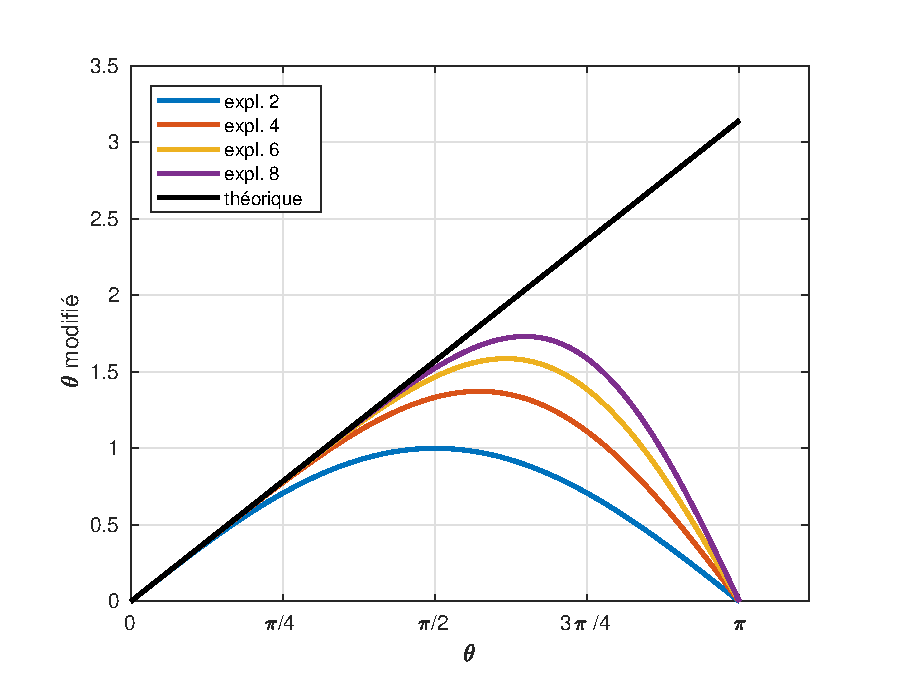
\includegraphics[scale=.6]{freq_classic.eps}
\end{center}
\caption{Représentation de $i Q_{2P}\left( \exp(i \theta) \right)$ en fonction de $\theta$ pour les schémas d'approximation explicites $\delta_{x,P}$ d'ordres 2, 4, 6 et 8.}
\label{fig:freq_classic}
\end{figure}

On définit $D_{2P} \in \mathbb{M}_N(\mathbb{R})$ la matrice associée à l'opérateur $\delta_{2P,x}$ :
\begin{equation}
D_{2P} = \dfrac{1}{h} Q_{2P}(T).
\end{equation}
La relation suivante est alors vérifiée
\begin{equation}
\vec_1(\delta_{2P,x} \mathfrak{u}) = D_{2P} \vec_1 ( \mathfrak{u} )
\end{equation}
pour tout $\mathfrak{u} \in l^2_{h,per}$.

Par exemple, le schéma centré d'ordre 2 $\delta_x = \delta_{2,x}$ est associée à la matrice
\begin{equation}
D_2 = \dfrac{1}{2h}
\begin{bmatrix}
0 & 1 &   &   &   & -1 \\ 
-1 & 0 & 1 &   & (0) &   \\ 
  & -1 & 0 & 1 &   &   \\ 
  &   & \ddots & \ddots & \ddots &   \\ 
  & (0) &   & -1 & 0 & 1 \\ 
1 &   &   &   & -1 & 0
\end{bmatrix} 
\end{equation}

\begin{proposition}
Les valeurs propres de $D_{2P}$ sont données par $\dfrac{1}{h}Q_{2P}(\omega^k)$ avec $-N/2 +1 \leq k \leq N/2$. Chaque valeur propre est associée à un vecteur propre $\vec_1{\mathfrak{u}^k}$.
\end{proposition}

\begin{proposition}
La matrice $D_{2P}$ est antisymétrique.
\end{proposition}

\begin{proof}
Montrons que $D_{2P}^T = - D_{2P}$ :
\begin{align*}
D_{2P}^T & = \dfrac{1}{h} Q_{2P}(T)^T \\
	& = \dfrac{1}{h} \left( \gsum_{j=1}^P \dfrac{a_j}{2j} (T^j - T^{N-j}) \right)^T\\
	& = \dfrac{1}{h}\gsum_{j=1}^P \dfrac{a_j}{2j} ((T^j)^T - (T^{N-j})^T) \\
	& = \dfrac{1}{h}\gsum_{j=1}^P \dfrac{a_j}{2j} (T^{N-j} - T^{j}) \\
	& = - \dfrac{1}{h} \gsum_{j=1}^P \dfrac{a_j}{2j} (T^j - T^{N-j}) \\
	& = - D_{2P}
\end{align*}
d'où le résultat.
\end{proof}





























\subsection{Opérateurs Hermitiens périodiques 1D}

Dans son article \cite{Lele1991}, S. K. Lele présente une méthode permettant d'approcher la dérivée en un point en ajoutant une partie implicite au schéma de la forme \eqref{eq:explicite_dx}. Dans ce chapitre, nous ne considérons que les schémas à 3 points implicites. Définissons l'opérateur $\sigma_{3,x}$ par :

\begin{equation}
(\sigma_{x} \mathfrak{u})_j = (1-2\beta) \mathfrak{u}_j + \beta \left( \mathfrak{u}_{j+1} + \mathfrak{u}_{j-1} \right)
\end{equation}

\begin{theoreme}
Si les coefficients réels $\beta$ et $(a_i)_{1 \leq i \leq P}$ sont solutions de 
\begin{equation}
\left\lbrace
\begin{array}{rcl}
\gsum_{p=0}^P a_p & = & 1 \\
\gsum_{p=0}^P a_p \dfrac{p^{2n}}{2n+1} & = & 2 \beta  \text{ pour } n=1,2,...P
\end{array}
\right.
\label{eq:hermitian_system}
\end{equation}
et si $u$ est une fonction de $\mathcal{C}^{2P+3}$, alors pour tout $0 \leq i \leq N-1$, on a 
\begin{equation}
(\delta_{P,x} u^*)_i - (\sigma_{3,x} u'^*)_i = \\
h^{2P+2} \left( \gsum_{p=0}^P a_p  \dfrac{j^{2P+2} P}{(2P+3)!}  - \dfrac{2\beta}{(2P+2)!}   \right)u^{(2P+3)}(\rho)
\end{equation}
avec $\rho \in [x_{i-P}, x_{i+P}]$.
\end{theoreme}

\begin{proof}
Soit $u : x \in \Omega \mapsto u(x) \in \mathbb{R}$ une fonction de classe $\mathcal{C}^{2P+3}( \Omega)$ et $u^*$ la fonction de grille correspondante.

On considère les développements de Taylor :
\begin{equation}
\begin{array}{rcl}
u(x_i + ph) & = & u(x_i) + p h u'(x_j) + \cdots + \dfrac{(ph)^k}{k!}u^{(k)}(x_i) + \cdots +\dfrac{(ph)^{2P+3}}{(2P+3)!} u^{(2P+3)}(\xi_p)\\
u(x_i - ph) & = & u(x_i) - p h u'(x_j) + \cdots + \dfrac{(-ph)^k}{k!}u^{(k)}(x_i) + \cdots +\dfrac{(-ph)^{2P+3}}{(2P+3)!} u^{(2P+3)}(\eta_p)
\end{array}
\end{equation}
avec $\xi_p \in [x_i, x_i+ph]$ et $\eta_p \in [x_i-ph, x_i]$. En combinant ces deux égalités, on a
\begin{equation}
\dfrac{\tau_pu^*_i - \tau_{-p} u^*_i}{2ph} = u'(x_i) + \cdots + \dfrac{(ph)^{k-1}(1 - (-1)^k)}{2 \cdot k!} u^{(k)}(x_i) + \cdots +\dfrac{(ph)^{2P+2}}{2(2P+3)!} \left( u^{(2P+3)}(\xi_p) + u^{(2P+3)}(\eta_p) \right)
\label{eq:preuve_herm1}
\end{equation}

D'autres part, on a 
\begin{equation}
(1-2\beta) u'^*_i + \beta \left( \tau_1 u'^*_{i} + \tau_{-1} u'^*_{i} \right) = u'^*_i +  \gsum_{k=1}^{2P+1} \beta \dfrac{h^{k}}{k!} \left( 1 + (-1)^k \right) u^{(k+1)}(x_i)+ \beta \dfrac{h^{2P+2}}{(2P+2)!} \left(u^{(2P+3)}(\varrho) + u^{(2P+3)}(\sigma) \right) 
\label{eq:preuve_herm2}
\end{equation}
avec $\varrho \in [x_i, x_i + h]$ et $\sigma \in [x_i, x_i - h]$. 

On remarque directement que \eqref{eq:preuve_herm2} et $\gsum_{p=0}^P a_p  \eqref{eq:preuve_herm1}$ coïncident pour les puissances de $h$ impaires. 

Pour les autres valeurs, l'égalité est vrai si les coefficients $a_p$ et $\beta$ sont solutions de \eqref{eq:hermitian_system}. L'erreur de troncature prend directement la forme 

\begin{multline}
(\delta_{P,x} u^*)_i - (\sigma_{3,x} u'^*)_i = \\
h^{2P+2} \left( \gsum_{p=0}^P a_p  \dfrac{j^{2P+2}}{2(2P+3)!} \left( u^{(2P+3)}(\xi_j) + u^{(2P+3)}(\eta_j) \right) - \dfrac{\beta}{(2P+2)!} \left(u^{(2P+3)}(\varrho) + u^{(2P+3)}(\sigma) \right) \right)
\end{multline}
On conclut alors en utilisant le théorème des valeurs intermédiaires.
\end{proof}

\begin{proposition}
Le système \eqref{eq:hermitian_system} admet une unique solution.
\end{proposition}






% disc.tex
\chapter{Analyse numérique}

\section{Opérateur de filtrage }

\subsection{Opérateur de filtrage en dimension 1}

Lors de la discrétisation via un schéma aux différences finies et suite à la discrétisation en temps, des oscillations parasites du type "+1/-1" peuvent apparaître. Il s'agit de phénomènes haute fréquences qui peuvent provoquer des instabilités numériques. 

Si $\mathfrak{u}$ est une fonction de grille périodique, on note le filtre passe-bas $\mathcal{F}\mathfrak{u}$. Dans la pratique, nous cherchons $\mathcal{F}$ sous la forme 

\begin{equation}
\mathcal{F} = \gsum_{k=0}^F a_k \dfrac{\tau^k + \tau^{-k}}{2}
\label{eq:ftr}
\end{equation}

Les coefficients $(a_k)_{0 \leq k \leq F}$ sont déterminés de manière à supprimer les phénomènes oscillants hautes fréquences (figure \ref{fig:hf_waves}) de la formes $\mathfrak{u}$ avec 
\begin{equation}
\mathfrak{u}_j = (-1)^j
\end{equation}

\begin{figure}[htbp]
\begin{center}
\begin{tikzpicture}[scale=1.4]
	\draw (-4,1) -- (-3,-1) ;
	\draw (-3,-1) -- (-2,1) ;
	\draw (-2,1) -- (-1,-1) ;
	\draw (-1,-1) -- (0,1) ;
	\draw (0,1) -- (1,-1) ;
	\draw (1,-1) -- (2,1) ;
	\draw (2,1) -- (3,-1) ;
	\draw (3,-1) -- (4,1) ;
	
	\draw (4,0) -- (-4,0) ;
	\foreach \k in {-3,...,3}
		{\draw  (\k,0) node[color=blue] {$\bullet$} ;
	   	\draw (\k,0) node {$\circ$} ;
	   	}
\end{tikzpicture}
\end{center}
\caption{Ondes de type "+1/-1".}
\label{fig:hf_waves}
\end{figure}


En considérant cette fonction de grille, on cherche $(a_k)_{0\leq k \leq F}$ tels que $\mathcal{F} \mathfrak{u} = \mathfrak{0}$, soit :
\begin{equation}
\mathcal{F}\mathfrak{u}_i = \gsum_{k=0}^F a_k \dfrac{\mathfrak{u}_{i+k} + \mathfrak{u}_{i-k}}{2} = \gsum_{k=0}^F a_k  \dfrac{(-1)^{i+k} + (-1)^{i-k}}{2} = 0.
\end{equation}
Cette équation est équivalente à 
\begin{equation}
\gsum_{k=0}^F a_k (-1)^k = 0
\label{eq:ftr_ftrcond}
\end{equation}
La relation \eqref{eq:ftr_ftrcond} nous donne une condition alors qu'il y a $F+1$ paramètres à déterminer. Il reste $F$ degrés de libertés dans l'opérateur de filtrage. Le choix qui est fait est de maximiser l'ordre du filtrage de manière à perturber un minimum la donnée initiale tout en supprimant les ondes parasites.

Le filtre doit conserver les très basses fréquences, lorsque $\mathfrak{u} = \mathfrak{1}$, on doit alors $\mathcal{F}\mathfrak{u} = \mathfrak{1}$.
C'est à dire que les coefficients $(a_k)_{0 \leq k \leq F}$ vérifient la relation de consistance
\begin{equation}
\gsum_{k=0}^F a_k = 1
\label{eq:ftr_conscond}
\end{equation}

Enfin, on remarque que si $u : x \in \Omega \mapsto u(x) \in \mathbb{R}$ et si $u^*$ est la fonction de grille associée à $u$, alors on a 
\begin{equation}
\begin{array}{rcl}
u(x_i + kh) & = & u(x_i) + p k u'(x_j) + \cdots + \dfrac{(kh)^l}{l!}u^{(l)}(x_i) + \cdots +\dfrac{(kh)^{2F}}{2F!} u^{(2F)}(\xi_k)\\
u(x_i - kh) & = & u(x_i) - p k u'(x_j) + \cdots + \dfrac{(-kh)^l}{l!}u^{(l)}(x_i) + \cdots +\dfrac{(-kh)^{2F}}{2F!} u^{(2F)}(\eta_k)
\end{array}
\end{equation}
avec $\xi_k \in [x_i, x_i+kh]$ et $\eta_k \in [x_i-kh, x_i]$. Alors par combinaison linéaire en considérant \eqref{eq:ftr_conscond} vérifiée, 
\begin{equation}
\mathcal{F}u^* - u^* = \gsum_{l=1}^{2F-1} \gsum_{k=0}^F \dfrac{a_k}{2} \underbrace{\dfrac{(kh)^l + (-kh)^l}{l!}}_{=0 \text{ pour } l \text{ impair.}}u^{(l)}(x_i) + \gsum_{k=0}^F \dfrac{a_k}{2}\dfrac{(kh)^{2F}}{2F!} \left( u^{(2F)}(\xi_k) + u^{(2F)}(\eta_k) \right)
\end{equation}
Ainsi, la condition de précision est 
\begin{equation}
\gsum_{k=0}^F a_k k^{2l} = 0 \text{ pour } 1 \leq l \leq F-1.
\label{eq:ftr_prescond}
\end{equation}

\begin{theoreme}
Soit $F \in \mathbb{N}^{\star}$. Il existe un unique $(a_k)_{0 \leq k \leq F}$ tel que $\mathcal{F}$ soit à la fois consistant en vérifiant \eqref{eq:ftr_conscond}, précis en vérifiant \eqref{eq:ftr_prescond} et soit un filtre passe bas en satisfesant \eqref{eq:ftr_ftrcond}. L'erreur de troncature du filtre est alors donnée par 
\begin{equation}
\mathcal{F}u^* - u^* = h^{2F} \gsum_{k=0}^F \dfrac{a_k}{2} \dfrac{k^{2F}}{2F!} \left( u^{(2F)}(\xi_k) + u^{(2F)}(\eta_k) \right).
\end{equation}
\label{prop:filter_def}
\end{theoreme}

\begin{proof}
La forme de l'erreur de troncature a déjà été vue, il reste à prouver l'unicité.

Après avoir retiré \eqref{eq:ftr_ftrcond} à \eqref{eq:ftr_conscond}, dire qu'il existe une unique $(a_j)_{0 \leq j \leq J}$ satisfesant les conditions est équivalent à dire que la matrice

\begin{equation}
A=\begin{bmatrix}
1 &  1  &  1  &  1  &  1  &  1  & \cdots\\  
0 &  2  &  0  &  2  &  0  & 2  & \cdots\\
0 &  1  & 2^2 & 3^2 & 4^2 & 5^2 & \cdots\\
0 &  1  & 2^4 & 3^4 & 4^4 & 5^4 & \cdots\\
0 &  1  & 2^6 & 3^6 & 4^6 & 5^6 & \cdots\\
&&& \vdots &  \vdots &
\end{bmatrix} \in \mathcal{M}_{J+1} \left( \mathbb{R} \right)
\end{equation}
est inversible car $a = [a_0, a_1, \cdots, a_J]^T$ est solution de 
\begin{equation}
A a = e_1
\end{equation}
avec $e = [1,1/2, 0,\cdots,0]^T$. En développant la seconde ligne de $A$, on a
\begin{equation}
\det ( A ) = \begin{vmatrix} 
2  &  0  &  2  &  0  & 2  & \cdots\\
1  & 2^2 & 3^2 & 4^2 & 5^2 & \cdots\\
1  & 2^4 & 3^4 & 4^4 & 5^4 & \cdots\\
1  & 2^6 & 3^6 & 4^6 & 5^6 & \cdots\\
& & \vdots &  \vdots &
\end{vmatrix} = 2 \sum_{k=1}^{\lfloor\frac{F-1}{2}\rfloor} \Delta_{2k+1}
\end{equation}
avec $\Delta_k$ donné par
\begin{equation}
\Delta_k = \begin{vmatrix} 
1 & 2^2 & \cdots & (k-1)^2 & (k+1)^2 & \cdots\\
1 & 2^4 & \cdots & (k-1)^4 & (k+1)^4 & \cdots\\
1 & 2^6 & \cdots & (k-1)^6 & (k+1)^6 & \cdots\\
&&& \vdots &  \vdots &
\end{vmatrix} = \dfrac{((F-1)!)^2}{k^2} \begin{vmatrix} 
1 & 1 & \cdots & 1 & 1 & \cdots\\
1 & (2^2)^1 & \cdots & ((k-1)^2)^1 & ((k+1)^2)^1 & \cdots\\
1 & (2^2)^2 & \cdots & ((k-1)^2)^2 & ((k+1)^2)^2 & \cdots\\
&&& \vdots &  \vdots &
\end{vmatrix}
\end{equation}
On reconnait alors un déterminant de Van-Der-Monde, donc $\Delta_k = \prod_{1 \leq i < j \leq F-1} \left( \alpha_j - \alpha_i \right)$, avec 
\begin{equation}
\alpha_j = \left\lbrace
\begin{array}{ll}
j^2 & \text{ avec } 1 \leq j \leq k-1\\
(j+1)^2 & \text{ avec } k \leq j \leq J-2\\
\end{array}
\right.
\end{equation}
Alors si $i<j$, on a $\alpha_i < \alpha_j$, donc $\Delta_k>0$ et même $\det A$ est une somme de déterminants tous strictements positifs donc $\det A > 0$. $A$ est inversible et le résultat est prouvé.
\end{proof}
Quelques filtres particuliers sont donnés dans la table \ref{tab:filter} en fonction de leur ordre de précision.

\begin{table}[htbp]
\begin{center}
\begin{tabular}{|c||cccccc|}
\hline
\textbf{Ordre de précision} & $a_0$ & $a_1$ & $a_2$ & $a_3$ & $a_4$ & $a_5$ \\
\hline \hline
$2$ & $1/2$ & $1/2$ & & & & \\
\hline
$4$ & $10/16$ & $8/16$ & $-2/16$ & & & \\
\hline
$6$ & $44/64$ & $30/64$ & $-12/64$ & $2/64$ & & \\
\hline
$8$ & $186/256$ & $112/256$ & $-56/256$ & $16/256$ & $-2/256$ & \\
\hline
$10$ & $772/1024$ & $420/1024$ & $-240/1024$ & $90/1024$ & $-20/1024$ & $2/1024$ \\
\hline
\end{tabular}
\end{center}
\caption{Exemples de filtres de la forme \eqref{eq:ftr} et leurs ordres de précision.}
\label{tab:filter}
\end{table}

Dans la suite, nous supposerons que $(a_k)_{0 \leq k \leq F}$ satisfait les conditions \eqref{eq:ftr_conscond}, \eqref{eq:ftr_prescond} et \eqref{eq:ftr_ftrcond}.
Les valeurs propres et fonctions propres de $\mathcal{F}$ sont issues de la proposition \ref{prop:eigen_P(tau)}. Le résultat est immédiat.

\begin{theoreme}
Les valeurs propres de $\mathcal{F}$ sont données par $\beta^k$ avec 
\begin{equation}
\beta^k = \gsum_{f=0}^F a_k \cos \left( \dfrac{2 \pi k f}{N} \right)
\end{equation}
pour tout $0 \leq k \leq N-1$, $\beta^k$ est associé à la fonction propre $\mathfrak{u}^k$ telle que 
\begin{equation}
\mathfrak{u}^k_j = \exp \left[ i j \dfrac{2 \pi k}{N} \right].
\end{equation}
\end{theoreme}

On définit le \textit{symbole} du filtre $\mathcal{F}$ par la fonction $\beta : \theta \in [0, \pi] \mapsto \beta(\theta) \in \mathbb{R}$ donnée par :
\begin{equation}
\beta( \theta ) = \gsum_{f=0}^F a_k \cos \left( f \theta \right)
\end{equation}

\begin{proposition}
Il existe un unique polynôme $P$ de degré $F$ tel que 
\begin{equation}
\beta(\theta) = P(\cos \theta )
\end{equation}
De plus,
\begin{equation}
P(x) = 1 -\dfrac{1}{(-2)^F} (X - 1)^F.
\end{equation}
\end{proposition}

\begin{proof}
Soit $\theta \in [0, \pi]$, 
\begin{equation}
\beta(\theta) = \gsum_{f=0}^F a_f \cos \left( f \theta \right) = \gsum_{f=0}^F a_f T_f ( \cos \theta )
\end{equation}
où $T_f \in \mathbb{R}_f [X]$ est le $k-$ieme polynome de Tchebytchev. 
Ainsi il existe $P \in \mathbb{R}_F [x]$ tel que $\beta( \theta ) = P( \cos \theta )$. Ce polynôme est unique. Montrons que 
\begin{equation}
P(x) = 1 -\dfrac{1}{(-2)^F} (X - 1)^F.
\end{equation}
convient.

\begin{itemize}
\item on montre facilement que 
\begin{equation}
P( \cos 0 ) = 1 -\dfrac{1}{(-2)^F} (\cos 0 - 1)^F = 1,
\end{equation}
de même,
\begin{equation}
P( \cos \pi ) = 1 -\dfrac{1}{(-2)^F} (\cos \pi - 1)^F 1 -\dfrac{(-2)^F}{(-2)^F} = 0.
\end{equation}
\item On rappelle la formule de Fàa Di Bruno permettant de calculer la dérivée $n-$ième d'une composée. Si $f$ et $g$ sont des fonctions régulières, on a 
\begin{equation}
\dfrac{d^n}{dx^n} \left( f \circ g \right)(x) = \gsum_{k=1}^n f^{(k)}\left( g(x) \right) B_{n,k}\left( g'(x), g''(x), \cdots , g^{n-k+1}(x) \right)
\end{equation}
où $B_{n,k}$ est un polynôme de Bell. En utilisant cette formule avec $f = P$ et $g = \cos$, évaluée en $\theta = 0$, on montre que :
\begin{equation}
\dfrac{d^n}{d\theta^n} \left( P \circ \cos \right)(0) = \gsum_{k=1}^n P^{(k)}\left(1\right) B_{n,k}\left( -1,0,1,0, \cdots\right)
\end{equation}
Or, $P^{(k)}\left(1\right) = 0$ pour tout $k \geq 1$. Donc 
\begin{equation}
\dfrac{d^n}{d\theta^n} \left( P \circ \cos \right)(0) = 0
\end{equation}
\end{itemize}
Le polynôme $P$ convient et 
\begin{equation}
\beta( \theta ) = 1 - \dfrac{1}{(-2)^F}(\cos \theta -1)^F.
\end{equation}
\end{proof}

\begin{proposition}
Pour tout $\theta \in [0, \pi]$, on a 
\begin{equation}
0 \leq \beta ( \theta ) \leq 1
\end{equation}
\end{proposition}

\begin{proof}
Supposons qu'il existe $\theta \in [0, \pi]$ tel que $\beta(\theta) < 0$ ou $\beta(\theta) > 1$. Comme $\beta(0)=1$ et $\beta(\pi) = 0$, il existe $\tilde{\theta} \in ]0, \pi[$ tel que 
\begin{equation}
\beta'(\tilde{\theta}) = - \sin \tilde{\theta} P'(\cos \tilde{\theta} ) = 0
\end{equation}
Or $\sin \tilde{\theta} \neq 0$ pour $\tilde{\theta} \in ]0, \pi[$.
De plus, 
\begin{equation}
P'(X) = \dfrac{F}{(-2)^F}(X-1)^{F-1}
\end{equation}
donc en prenant $X = \cos \tilde{\theta}$,
\begin{equation*}
P'(X) = 0 \Leftrightarrow \cos \tilde{\theta} = 1
\end{equation*}
Ce qui est impossible pour $\tilde{\theta} \in ]0, \pi[$. Donc par l'absurde, le résultat est vérifié.
\end{proof}

La fonction $\beta$ permet de considérer le comportement du filtre sur les différentes fréquences $\theta \in [0, \pi]$. Les basses fréquences sont bien conservées alors que les hautes fréquences ($\theta$ proche de $\pi$) sont atténuées. Cette observation est visible sur la figure \ref{fig:freq_filter} représentant la fonction $\beta : \theta \mapsto \beta(\theta)$ associée aux filtres d'ordre 2, 4, 6, 8 et 10. 

\begin{figure}[htbp]
\begin{center}
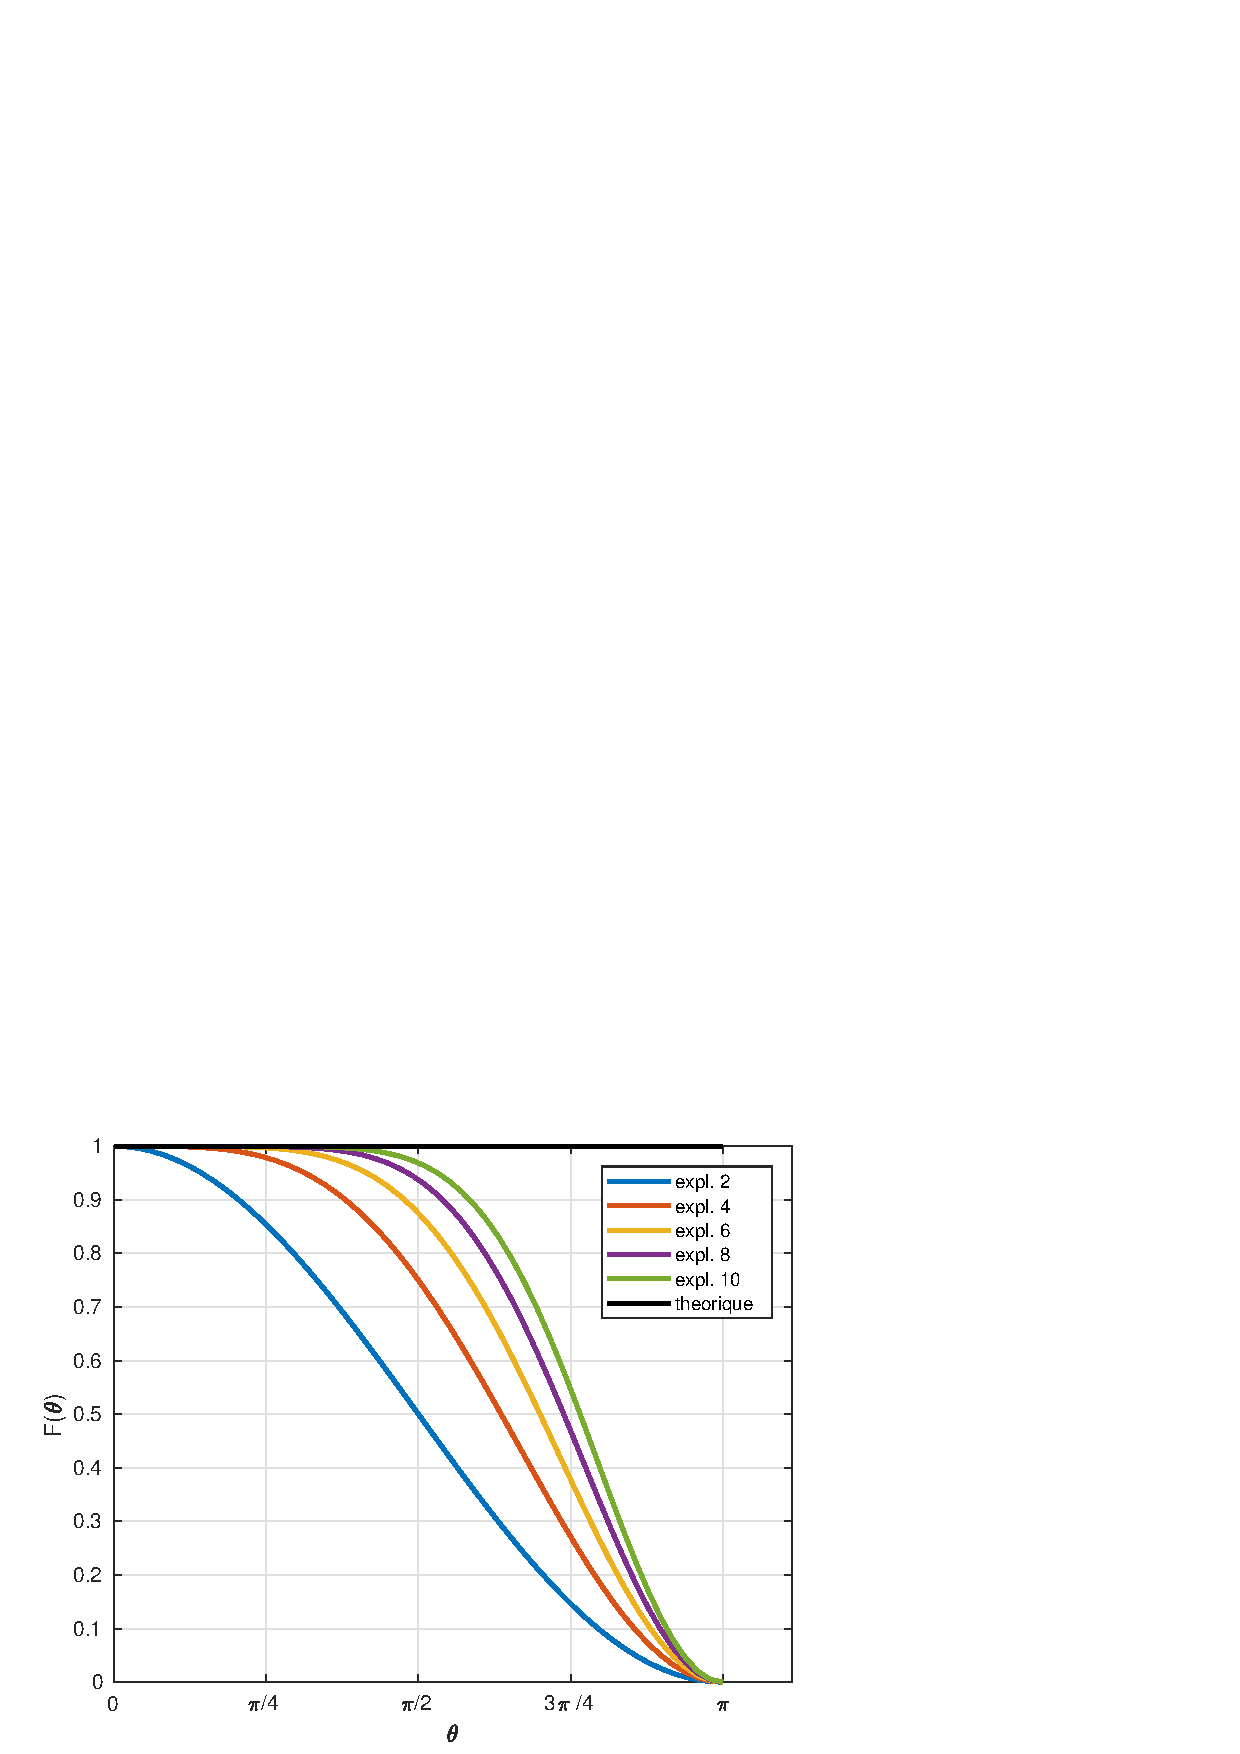
\includegraphics[scale=0.7]{freq_filter.png}
\end{center}
\caption{Fonction d'amplification $\beta$ pour les filtres explicites d'ordre 2, 4, 6, 8 et 10.}
\label{fig:freq_filter}
\end{figure}
Comme on s'y attendais, un filtre d'ordre élevé laisse passer un plus grand nombre de basses fréquences. Dans le tableau \ref{tab:filter_095}, on représente la fréquence $\theta_{0.95}$ maximale qui est conservée à $95\%$. Comme la fonction $\beta$ est strictement décroissante sur $[0,\pi]$, c'est une bijection de $[0,pi]$ dans $[0,1]$ et on a 
\begin{equation}
\theta_{0.95} = \beta^{-1}(0.95).
\end{equation}

\begin{table}
\begin{center}
\begin{tabular}{|c||c|}
\hline
\textbf{Ordre du filtre} & \textbf{Fréquence conservée à } $95\%$\\
\hline
\hline
$10$&$1.6695$\\
$8$&$1.5165$\\
$6$&$1.3045$\\
$4$&$0.9851$\\
$2$&$0.4510$\\
\hline
\end{tabular}
\end{center}
\caption{Fréquence conservée à $95\%$ en fonction de l'ordre du filtre.}
\label{tab:filter_095}
\end{table}

En pratique, cette fréquence $\theta_{0.95}$ est donnée en résolvant $\beta(\theta_{0.95})=0.95$ par 
\begin{equation}
\theta_{0.95} = \arccos \left[ 1-2 (0.05)^{1/F} \right].
\end{equation}
On remarque directement que la fonction $F \mapsto \theta_{0.95}$ est croissante, ce qui confirme que lorsque l'ordre de précision croit, $J$ croit et $\theta_{0.95}$ croit donc le filtre conserve un plus grand nombre de fréquences. De plus, 
\begin{equation}
\lim_{F \rightarrow \infty} \theta_{0.95} = \pi.
\end{equation}
Ce qui confirme la prise en compte d'un grand nombre de fréquence lorsque l'on augmente l'ordre du filtre. Cependant lorsque l'ordre du filtre augmente, l'effet de filtrage des hautes fréquences diminue.

Si $\mathfrak{u}$ est une fonction de grille, on pose $U$ et $\tilde{U}$ les vecteurs de $\mathbb{R}^N$ tel que
\begin{equation}
U = \begin{bmatrix}
\mathfrak{u}_1\\
\mathfrak{u}_2\\
\vdots \\
\mathfrak{u}_N\\
\end{bmatrix} \text{ et } 
\tilde{U} = \begin{bmatrix}
\mathcal{F}\mathfrak{u}_1\\
\mathcal{F}\mathfrak{u}_2\\
\vdots \\
\mathcal{F}\mathfrak{u}_N\\
\end{bmatrix}
\end{equation}
Alors $U$ et $\tilde{U}$ vérifient la relation
\begin{equation}
\tilde{U} = M F
\end{equation}
avec $M \in \mathcal{M}_N \left( \mathbb{R} \right)$ la matrice associée au filtrage des données en dimension 1 (dans le cas $F=2$):
\begin{equation}
M = \dfrac{1}{2}
\begin{bmatrix}
2a_0 & a_1 & a_2 &   &   &   & a_2 & a_1 \\ 
a_1 & 2 a_0 & a_1 & a_2 &   &   &   & a_2 \\ 
a_2 & a_1 & 2a_0 & a_1 & a_2 & (0) &   &   \\ 
  & a_2 & a_1 & 2a_0 & a_1 & a_2 &   &   \\ 
  &   & \ddots & \ddots & \ddots & \ddots & \ddots &   \\ 
  &   & (0) & a_2 & a_1 & 2 a_0 & a_1 & a_2 \\ 
a_2 &   &   &   & a_2 & a_1 & 2a_0 & a_1 \\ 
a_1 & a_2 &   &   &   & a_2 & a_1 & 2a_0
\end{bmatrix} 
\end{equation}
ou plus généralement 
\begin{equation}
M_{i,j} = \left\lbrace
\begin{array}{cl}
a_0 & \text{ si } i=j \\
\dfrac{1}{2} a_k & \text{ si } i+j \equiv k [N]\\
0 & \text{ sinon.}
\end{array}
\right.
\end{equation}
Il est clair que la matrice $M$ est symétrique.








\subsection{Opérateur de filtrage en géométrie cartésienne 2D}

Dans cette partie, nous utilisons toujours les notations de la section \ref{sec:notation_2D} en contexte périodique. Définissons les opérateurs de filtrage dans les directions $x$ et $y$ par
\begin{eqnarray*}
\mathcal{F}_x = \gsum_{k=0}^F a_k \dfrac{\tau_x^k + \tau_x^{-k}}{2} \\
\mathcal{F}_y = \gsum_{k=0}^F a_k \dfrac{\tau_y^k + \tau_y^{-k}}{2} \\
\end{eqnarray*}

Avec $(a_k)_{0 \leq k \leq F}$ vérifiant \ref{prop:filter_def}. Comme la géométrie est cartésienne, on remarque que 
\begin{equation}
\mathcal{F}_x \circ \mathcal{F}_y = \mathcal{F}_y \circ \mathcal{F}_x.
\end{equation}
Ce qui est faux lorsque la métrique n'est pas orthogonale.
La proposition \ref{prop:filter_def} permet de vérifier la consistance des opérateurs de filtrages.
Si $u : (x,y) \in \Omega \mapsto u(x,y) \in \mathbb{R}$ est fonction de $\mathcal{C}^{2F}$ alors :
\begin{eqnarray*}
\mathcal{F}_x u^*_{i,j} - u^*_{i,j} & = & C_xh^{2F}\\
\mathcal{F}_y u^*_{i,j} - u^*_{i,j} & = & C_yh^{2F}
\end{eqnarray*}
où $C_x$ et $C_y$ sont des constantes indépendantes de $h$.
En particulier, en composant les opérateurs, on peut définir un nouvel opérateur de filtrage. En effet  
\begin{equation}
(\mathcal{F}_x \circ \mathcal{F}_y) u_{i,j}^* - u_{i,j}^* = Ch^{2F}.
\end{equation}

L'écriture matricielle de l'opérateur de filtrage est donnée par la proposition suivante :
\begin{proposition}
Soit $\mathbf{u}$ une fonction de grille. Alors les opérateurs de filtrages s'écrivent à l'aide de matrices comme :
\begin{equation}
\left\lbrace
\begin{array}{rcl}
\text{vec}_2 (\mathcal{F}_x \mathbf{u}) & = & (Id \otimes M) \text{vec}_2 (\mathbf{u})\\
\text{vec}_2 (\mathcal{F}_y \mathbf{u}) & = & (M \otimes Id) \text{vec}_2 (\mathbf{u})\\
\end{array}
\right.
\end{equation}
\end{proposition}
Comme la matrice $M$ est symétrique, il est immédiat que $Id \otimes M$ et $M \otimes Id$ sont symétriques aussi.
















\section{Discrétisation temporelle}

La résolution numérique des équations considérées se fait par la méthode des lignes. Il s'agit de discrétiser dans un premier lieux les opérateurs spatiaux pour aboutir à une équations semi-discrétisée. Il ne reste que la dimension temporelle à considérer : il s'agit de la résolution numérique d'une équation aux dérivées ordinaires. Nous considérons ici des EDO de la forme
\begin{equation}
\dfrac{d q}{dt} = J_{\Delta} (q)
\label{eq:edo}
\end{equation}
avec la condition initiale $q(0)=q_0$. 
Ce choix de méthode est particulièrement pratique. La discrétisation spatiale et la discrétisation temporelle sont séparées, cela facilite le développement de nouvelles méthodes de discrétisations qui peuvent aisément être changées.

\subsection{Discrétisation de Runge-Kutta d'ordre 4}

Le schéma de résolution temporelle de référence que nous considérons est le schéma de Runge-Kutta d'ordre 4 (RK4). Si nous connaissons l'état de $q$ au temps $t^n = n \Delta t$ (que nous noterons $q^n$) alors nous cherchons à déterminer de façon explicite une valeur approchée de $q$ au temps $t^{n+1} = (n+1) \Delta t$. C'est à dire que nous cherchons $Q$ tel que
\begin{equation}
q^{n+1} = Q(q^n)
\end{equation}
Le schéma de Runge-Kutta d'ordre 4 s'écrit suivant l'algorithme \ref{alg:RK4}.

\begin{center}
\begin{minipage}[H]{12cm}
  \begin{algorithm}[H]
    \caption{: RK4}\label{alg:RK4}
    \begin{algorithmic}[1]
    \State $q^0 = q_0$ connu,
    \For{$n=0,1, \ldots$}
             \State  $K^{(1)} = J_{\Delta} \left( q^n \right)$,
             \State  $K^{(2)} = J_{\Delta} \left( q^n + \dfrac{\Delta t}{2} K^{(1)}\right)$,
             \State  $K^{(3)} = J_{\Delta} \left( q^n + \dfrac{\Delta t}{2} K^{(2)}\right)$,
             \State  $K^{(4)} = J_{\Delta} \left( q^n + \Delta t K^{(3)}\right)$,  
             \State  $q^{n+1} = q^n  + \dfrac{\Delta t}{6} \left( K^{(1)} + 2 K^{(2)} + 2 K^{(3)} + K^{(4)} \right)$.
            \EndFor
    \end{algorithmic}
    \end{algorithm}
\end{minipage}
\end{center}

\begin{theoreme}
La méthode de résolution RK4 donnée dans l'algorithme \ref{alg:RK4} définie une méthode de résolution de \ref{eq:edo} d'ordre 4. Si $q : t \in \mathbb{R}^+ \mapsto \mathbb{R}^N$ est une fonction de $\mathcal{C}^5$ et $q^n = q(n \Delta t)$ alors
\begin{equation}
q((n+1) \Delta t) - q^{n+1} = \mathcal{O} \left( \Delta t^5 \right)
\end{equation}

\end{theoreme}

\subsection{Stabilité}

\subsection{Schéma filtré}















\section{Equation d'advection 1D}

\subsection{Discrétisation}

\subsection{Consistance et Stabilité}

\subsection{Relations de conservations}
% CS.tex
\chapter{Cubed-Sphere}

\section{Construction}

\section{Coordonnées}

\subsection{Tenseur métrique}

\subsection{Symboles de Christophel}
% opsph.tex
% opérateurs sphériques sur la sphère

\chapter{Approximation des opérateurs sphériques sur la Cubed-sphere}

La résolution des équations de type Shallow-Water \REF la sphère $\mathbb{S}_a^2$ demande le calcul approché d'opérateurs classiques. Les opérateurs différentiels sont indispensables pour la discrétisation spatiale. On pense en particulier aux opérateurs divergence, gradient ou rotationnel. Dans cette section, nous les définissons sur la Cubed-sphere. 
Nous avons vu dans le cas 1D qu'un opérateur de filtrage peut être utile pour supprimer les modes de type "$+1/-1$" qui perturbent le calcul lors de la discrétisation en temps. Nous définissons les opérateurs de filtrages permettant d'aboutir au filtrage qui sera utilisé dans la discrétisation temporelle des équations.
Dans ce chapitre, les notations employées telles que $\xi$, $\eta$, $\alpha$, ... sont celles employées dans le chapitre \REF concernant la Cubed-sphere.

\section{Opérateurs différentiels sur la Cubed-sphere}

\subsection{Définition des opérateurs}
Soit $\mathbf{x}_{i,j}^k$ un point de la Cubed-sphere avec $- N/2 \leq i,j \leq N/2$ et $k = (I) \cdots (VI)$. Alors il existe deux grands cercles $C_i^{(1)}$ et $C_j^{(2)}$ deux grands cercles tels que $\mathbf{x}_{i,j}^k \in C_i^{(1)} \cap C^{(2)}_j$. $\alpha$ et $\beta$ sont respectivement les angles paramétrant $C_i^{(1)}$ et $C_j^{(2)}$.

On a définit le gradient en $\mathbf{x}_{i,j}^k$ par 
\begin{equation}
\nabla_T h = \dfrac{\partial h}{\partial \alpha}_{|C^{(2)}_j} \mathbf{g}^{\alpha} + \dfrac{\partial h}{\partial \beta}_{|C^{(1)}_i} \mathbf{g}^{\beta},
\end{equation}
où $h \mathbf{x} \in \mathbb{S}_a^2 \mapsto h(\mathbf{x})$ est une fonction régulière sur la sphère.

Le cercle $C_i^{(1)}$ (resp. $C_j^{(2)}$) est une isocline $\xi = \xi_i$ (resp $\eta = \eta_j$) constant. D'après le théorème \eqref{th:gradient_xieta}, le gradient est calculable via la formule
\begin{equation}
\nabla_T h = \dfrac{\partial h}{\partial \xi}_{|\eta_j} \mathbf{g}^{\xi} + \dfrac{\partial h}{\partial \eta}_{|\xi_i} \mathbf{g}^{\eta}.
\end{equation}
On remarque que si l'on est capable de calculer les dérivées partielles $\partial_{\xi}$ et $\partial_{\eta}$ le long des grands cercles, alors on est capable de déterminer la valeur du gradient.

Soit $\mathbf{v} : \mathbf{x} \in \mathbb{S}_a^2 \mapsto \mathbf{v}(\mathbf{x}) \in \mathbb{T}_{\mathbf{x}} \mathbb{S}_a^2$ un champ de vecteur tangent à la sphère. On définit la \textit{divergence} et le \textit{rotationnel} de $\mathbf{v}$ notés $\nabla_T \cdot \mathbf{v}$ et $\nabla_T \wedge \mathbf{v}$.

\begin{definition}
Soit $\mathbf{v} : \mathbf{x} \in \mathbb{S}_a^2 \mapsto \mathbf{v}(\mathbf{x}) \in \mathbb{T}_{\mathbf{x}} \mathbb{S}_a^2$ un champ de vecteur régulier sur la sphère. Alors la divergence de $\mathbf{v}$ en $\mathbf{x} \in C_i^{(1)} \cap C_j^{(2)}$ est donnée par
\begin{equation}
\nabla_T \cdot \mathbf{v} = \dfrac{\partial \mathbf{v}}{\partial \alpha}_{|C^{(2)}_j} \cdot \mathbf{g}^{\alpha} + \dfrac{\partial \mathbf{v}}{\partial \beta}_{|C^{(1)}_i} \cdot \mathbf{g}^{\beta}.
\end{equation}
\label{def:divergence}
La notation $\cdot$ désigne le produit scalaire usuel dans $\mathbb{R}^3$.
\end{definition}
Le rotationnel d'un champ de vecteurs représente la tendance des lignes de courant de $\mathbf{v}$ à tourner autour d'un point. Il est définit par

\begin{definition}
Soit $\mathbf{v} : \mathbf{x} \in \mathbb{S}_a^2 \mapsto \mathbf{v}(\mathbf{x}) \in \mathbb{T}_{\mathbf{x}} \mathbb{S}_a^2$ un champ de vecteur régulier sur la sphère. Alors le rotationnel de $\mathbf{v}$ en $\mathbf{x} \in C_i^{(1)} \cap C_j^{(2)}$ est donnée par
\begin{equation}
\nabla_T \wedge \mathbf{v} =  \mathbf{g}^{\alpha} \wedge \dfrac{\partial \mathbf{v}}{\partial \alpha}_{|C^{(2)}_j} + \mathbf{g}^{\beta} \wedge \dfrac{\partial \mathbf{v}}{\partial \beta}_{|C^{(1)}_i}
\end{equation}
où $\wedge$ désigne le produit vectoriel.
\label{def:rotationnel}
\end{definition}
La \textit{vorticité} du champ de vecteurs $\mathbf{v}$ est la composante normale du rotationnel :
\begin{equation}
\vort ( \mathbf{v} ) = \left( \nabla_T \wedge \mathbf{v} \right) \cdot \mathbf{k}
\label{eq:vorticité}
\end{equation}
avec $\mathbf{k}$ le vecteur unitaire extérieur à la sphère en $\mathbf{x} \in \mathbb{S}_a^2$, il vérifie l'égalité
\begin{equation}
\mathbf{k} = \dfrac{1}{a} \mathbf{x}.
\end{equation}

En utilisant la proposition \ref{prop: g_alpha g_beta fct de g_xi g_eta}, il est facile de montrer que des égalités permettant de calculer les opérateurs à l'aide des dérivées en $\xi$ et en $\eta$.

\begin{theoreme}
Soit $h : \mathbf{x} \in \mathbb{S}_a^2 \mapsto h(\mathbf{x})$ une fonction régulière et $\mathbf{v} : \mathbf{x} \in \mathbb{S}_a^2 \mapsto \mathbf{v}(\mathbf{x}) \in \mathbb{T}_{\mathbf{x}} \mathbb{S}_a^2$ un champ de vecteurs régulier. Alors en $\mathbf{x}_{i,j}^k$ un point de la Cubed-Sphere, les égalités suivantes sont satisfaites :
\begin{itemize}
\item \textbf{Gradient} :
\begin{equation}
\nabla_T h = \dfrac{\partial h}{\partial \xi}_{|\eta_j} \mathbf{g}^{\xi} + \dfrac{\partial h}{\partial \eta}_{|\xi_i} \mathbf{g}^{\eta},
\end{equation}

\item \textbf{Divergence} :
\begin{equation}
\nabla_T \cdot \mathbf{v} = \dfrac{\partial \mathbf{v}}{\partial \xi}_{|\eta_j} \cdot \mathbf{g}^{\xi} + \dfrac{\partial \mathbf{v}}{\partial \eta}_{|\xi_i} \cdot \mathbf{g}^{\eta},
\end{equation}

\item \textbf{Rotationel} :
\begin{equation}
\nabla_T \cdot \mathbf{v} = \mathbf{g}^{\xi} \wedge \dfrac{\partial \mathbf{v}}{\partial \xi}_{|\eta_j} + \mathbf{g}^{\eta} \wedge \dfrac{\partial \mathbf{v}}{\partial \eta}_{|\xi_i}.
\end{equation}
\end{itemize} 
\end{theoreme}

Pour calculer une valeur approchée des opérateurs gradient, divergence et rotationnel aux points du maillage de la Cubed-Sphere, il faut calculer une valeur approchée de la dérivée d'une fonction le long d'un grand cercle. C'est à dire, calculer $f_{\xi,i,j}$ et $f_{\eta,i,j}$ tels que 
\begin{equation}
\left\lbrace
\begin{array}{rl}
f_{\xi,i,j} \rightarrow \partial_{\xi} f ( \mathbf{x}_{i,j}^k) & \text{ lorsque } \Delta \xi \rightarrow 0\\
f_{\eta,i,j} \rightarrow \partial_{\eta} f ( \mathbf{x}_{i,j}^k) & \text{ lorsque } \Delta \eta \rightarrow 0
\end{array}
\right.
\end{equation}
La section suivante consiste à détailler une procédure pour calculer ces dérivées partielles approchées et à déterminer l'erreur effectuée lors du calcul.





\subsection{Approximation de dérivées sur les grands cercles}

On pose $f : \mathbf{x}\in \mathbb{S}_a^2 \mapsto f(\mathbf{x})$ la fonction que l'on souhaite dérivée le long des grands cercles aux points du maillage de la Cubed-Sphere.
Si $\mathbf{x}_{i,j}^k$ est un point de la Cubed-Sphere avec $k = (I) \cdots (VI)$, ainsi que $-N/2 \leq i,j \leq N/2$. On souhaite calculer une valeur approchée de 
$
\partial_{\xi} f (\mathbf{x}_{i,j}^k) \text{ et } \partial_{\xi} f (\mathbf{x}_{i,j}^k)
$.
On suppose par exemple $k = (I)$ mais la méthode est la même sur les autres panels. Alors il existe deux grands cercles de la Cubed-Sphere $C_i^{(1)}$ et $C_j^{(2)}$ tels que 
\begin{equation}
\mathbf{x}_{i,j}^k \in C_i^{(1)} \cap C^{(2)}_j.
\end{equation}
$C^{(1)}_i$ est une isoligne en $\xi = \xi_i$ constant et $C^{(2)}_j$ est une isoligne en $\eta = \eta_j$ constant.
Pour calculer une valeur approchée de $\partial_{\xi} f (\mathbf{x}_{i,j}^{(I)})$, on souhaite connaître toutes les valeurs de $f$ aux points équirépartis le long du cercle $C^{(2)}_j$. On pose $\mathbf{m}_p$ avec $0 \leq p \leq 4N-1$ les points de $C^{(2)}_j$ construits de la manière suivante :
\begin{itemize}
\item si $0 \leq p \leq N$ alors $\mathbf{m}_p = \mathbf{x}^{(I)}_{p-N/2,j}$, il s'agit des points du cercle $C^{(2)}_j$ associés au panel $(I)$ sur le maillage. Ils sont représentés par des ronds bleus sur les figures \ref{fig:patron_cs} et \ref{fig: panel II_interp},
\item si $N+1 \leq p \leq 2N-1$ alors les points ne font pas partis du maillages. Il s'agit des des points d'intersections de $C^{(2)}_j$ avec les isoligne $\xi = \xi_i^{(II)}$ du panel $(II)$. C'est à dire l'intersection de $C^{(2)}_j$ avec les cercles de $(II_{\beta})$. Ces points sont représentés par les carrés bleus dans les figures \ref{fig:patron_cs} et \ref{fig: panel II_interp}. Les coordonnées de ces points ont été calculées dans la partie \REF.
\item si $2N \leq p \leq 3N$ alors $\mathbf{m}_p = \mathbf{x}^{(III)}_{p-3N/2}$. Il s'agit des points de la Cubed-Sphere du panel $(III)$ représentés par des ronds bleus sur la figure \ref{fig:patron_cs},
\item si $3N+1 \leq p \leq 4N-1$ alors $\mathbf{m}_p$ est constitués des points d'intersections de $C^{(2)}_j$ avec les cercles de $(IV_{\beta})$. Il ne s'agit pas de points de la grille. Ces points sont représentés par les carrés bleus dans la figure \ref{fig:patron_cs}.
\end{itemize}

\begin{figure}
\begin{center}
\begin{tikzpicture}[scale=2.5]
	\foreach \x in {1,...,7}
		{ \draw [color=gray!70, line width=0.8pt] (0.125*\x,1) -- (0.125*\x,2) ;
		\draw [color=gray!30] (0,1+0.125*\x) -- (1,1+0.125*\x) ;
		\draw [color=gray!30] (1+0.125*\x,1) -- (1+0.125*\x,2) ;
		\draw [color=gray!30] (1,1+0.125*\x) -- (2,1+0.125*\x) ;
		\draw [color=gray!70, line width=0.8pt] (2+0.125*\x,1) -- (2+0.125*\x,2) ;
		\draw [color=gray!30] (2,1+0.125*\x) -- (3,1+0.125*\x) ;
		\draw [color=gray!30] (3+0.125*\x,1) -- (3+0.125*\x,2) ;
		\draw [color=gray!30] (3,1+0.125*\x) -- (4,1+0.125*\x) ;
		\draw [color=gray!30] (1+0.125*\x,0) -- (1+0.125*\x,1) ;
		\draw [color=gray!30] (1,0.125*\x) -- (2,0.125*\x) ;
		\draw [color=gray!30] (1+0.125*\x,2) -- (1+0.125*\x,3) ;		
		\draw [color=gray!30] (1,2+0.125*\x) -- (2,2+0.125*\x) ;
		}
	

	\draw [line width=0.6pt] (1,3) -- (2,3) ; 
	\draw [line width=0.6pt] (0,2) -- (4,2) ; 	
	\draw [line width=0.6pt] (0,1) -- (4,1) ; 
	\draw [line width=0.6pt] (1,0) -- (2,0) ; 
	
	\draw [line width=0.6pt] (0,2) -- (0,1) ;
	\draw [line width=0.6pt] (1,3) -- (1,0) ;
	\draw [line width=0.6pt] (2,3) -- (2,0) ;
	\draw [line width=0.6pt] (3,2) -- (3,1) ;
	\draw [line width=0.6pt] (4,2) -- (4,1) ; 
	
	\draw (0.7,1.1) node[above]{$(IV)$} ; 
	\draw (1.3,1.1) node[above]{$(I)$} ; 
	\draw (2.7,1.7) node[above]{$(II)$} ;
	\draw (3.3,1.7) node[above]{$(III)$} ;  
	\draw (1.7,2.7) node[above]{$(V)$} ;  
	\draw (1.3,0.7) node[above]{$(VI)$} ; 
	
	\draw [samples=100,domain=0:1,color=blue] plot({\x},{1.5-(2*0.125)*cos(180*\x)});
	\draw [samples=100,domain=1:2,color=blue] plot({\x},{1.5+2*0.125});
	\draw [samples=100,domain=1:2,color=blue] plot({\x+1},{1.5-2*0.125*cos(180*\x)});
	\draw [samples=100,domain=3:4,color=blue] plot({\x},{1.5-2*0.125});
	\draw [>=stealth, <-] (0.05,1.25) -- (0.3,0.5) ;
	\draw  (0.3,0.5) node[right] {iso-$\eta$} ;
	
	\draw [samples=100,domain=0:1,color=red] plot({1.5-2*0.125*cos(180*\x)},{\x});
	\draw [samples=100,domain=1:2,color=red] plot({1.5+2*0.125},{\x});
	\draw [samples=100,domain=1:2,color=red] plot({1.5-2*0.125*cos(180*\x)},{\x+1});
	\draw [samples=100,domain=1:2,color=red] plot({4-2*0.125},{\x});
	\draw [>=stealth, <-] (1.5,0.5) -- (2.2,0.4) ;
	\draw  (2.2,0.4) node[right] {iso-$\xi$} ;
	
	\draw  (0,1+2*0.125) node[color=blue] {$\bullet$} ;
	\draw (0,1+2*0.125) node {$\circ$} ;
	
	\foreach \k in {0,...,8}
		{\draw  (1+0.125*\k,1.5+2*0.125) node[color=blue] {$\bullet$} ;
	   	\draw (1+0.125*\k,1.5+2*0.125) node {$\circ$} ;
	   	\draw  (3+0.125*\k,1+2*0.125) node[color=blue] {$\bullet$} ;
	   	\draw (3+0.125*\k,1+2*0.125) node {$\circ$} ;
	   	}
	   	
	\foreach \x in {1,...,7}
		{\draw  ({0.125*\x},{1.5-2*0.125*cos(180*0.125*\x)}) node[color=blue] {\begin{tiny}$\blacksquare$\end{tiny}} ;
	   	\draw ({0.125*\x},{1.5-2*0.125*cos(180*0.125*\x)}) node {\begin{tiny}$\square$\end{tiny}} ;
	   	\draw  ({2+0.125*\x},{1.5-2*0.125*cos(180*0.125*\x+180)}) node[color=blue] {\begin{tiny}$\blacksquare$\end{tiny}} ;
	   	\draw  ({2+0.125*\x},{1.5-2*0.125*cos(180*0.125*\x+180)}) node {\begin{tiny}$\square$\end{tiny}} ;
	   	}
	   	
	\draw [>=stealth, <-] (0.25,1.75) -- (0.125,2.5) ;
	\draw [>=stealth, <-] (0.625,1.85) -- (0.125,2.5) ;
	\draw  (0.125,2.5) node[above] {Lignes d'interpolation} ;
\end{tikzpicture}
\caption{Les grands cercles associés aux panels $(I)$ et $(III)$ ne sont pas passent pas par des points du la Cubed-Sphere sur les panels $(II)$ et $(IV)$.}
\label{fig:patron_cs}
\end{center}
\end{figure}




\begin{figure}[htbp]
\begin{center}
\begin{tikzpicture}[scale=2.2]
	\draw [line width=0.8pt] (0,0) circle (1cm);
    \shade[ball color=blue!10!white,opacity=0.20] (0,0) circle (1cm);	
	
	\filldraw[draw=black,fill=blue!30!white,opacity=0.20]
	plot [smooth,domain=-35:35] ({0.7*cos(\x)},{sin(\x)})
	-- plot [smooth,domain=55:125] ({cos(\x)},{0.7*sin(\x)})
	-- plot [smooth,domain=150:215] ({0.7*cos(\x)},{sin(\x)})
	-- plot [smooth,domain=240:300] ({cos(\x)},{0.7*sin(\x)})
	-- cycle;	
	\draw [samples=100,domain=48:132, color=gray!50] plot({cos(\x)},{0.35*sin(\x)});
	\draw [samples=100,domain=48:132, color=gray!50] plot({cos(\x)},{-.35*sin(\x)});
	\draw [samples=100,domain=46:134, color=gray!50] plot({cos(\x)},{0.175*sin(\x)});
	\draw [samples=100,domain=46:134, color=gray!50] plot({cos(\x)},{-.175*sin(\x)});
	\draw [samples=100,domain=50:130, color=gray!50] plot({cos(\x)},{0.525*sin(\x)});
	\draw [samples=100,domain=50:130, color=gray!50] plot({cos(\x)},{-.525*sin(\x)});
	\draw [samples=100,domain=45:135, color=gray!50] plot({cos(\x)},{0*sin(\x)});

	\draw [rotate=90, samples=100,domain=48:132, color=gray, line width=0.6pt] plot({cos(\x)},{0.35*sin(\x)});
	\draw [rotate=90, samples=100,domain=48:132, color=gray, line width=0.6pt] plot({cos(\x)},{-.35*sin(\x)});
	\draw [rotate=90, samples=100,domain=46:134, color=gray, line width=0.6pt] plot({cos(\x)},{0.175*sin(\x)});
	\draw [rotate=90, samples=100,domain=46:134, color=gray, line width=0.6pt] plot({cos(\x)},{-.175*sin(\x)});
	\draw [rotate=90, samples=100,domain=50:130, color=gray, line width=0.6pt] plot({cos(\x)},{0.525*sin(\x)});
	\draw [rotate=90, samples=100,domain=50:130, color=gray, line width=0.6pt] plot({cos(\x)},{-.525*sin(\x)});
	\draw [rotate=90, samples=100,domain=45:135, color=gray, line width=0.6pt] plot({cos(\x)},{0*sin(\x)});

	\filldraw[draw=black,fill=red!30!white,opacity=0.20]
	plot [smooth,domain=145:215] ({.7*cos(\x)},{sin(\x)})
	-- plot [smooth] (-.573,-.573) -- (-.707,-.707)
	-- plot [smooth,domain=215:145] ({cos(\x)},{sin(\x)})
	-- plot [smooth] (-.707,.707) -- (-.573,.573)
	-- cycle;	
	\draw [line width=0.8pt] (-.573,-.573) -- (-.707,-.707) ;
	\draw [line width=0.8pt] (-.573,.573) -- (-.707,.707) ;
	\draw [color=gray!50] (-.669,.260) -- (-.9321,.3622) ;
	\draw [color=gray!50] (-.669,-.260) -- (-.9321,-.3622) ;
	\draw [color=gray!50] (-.6946,.1259) -- (-.9840,.1783) ;
	\draw [color=gray!50] (-.6946,-.1259) -- (-.9840,-.1783) ;
	\draw [color=gray!50] (-.6427,.4022) -- (-.8477,.5305) ;
	\draw [color=gray!50] (-.6427,-.4022) -- (-.8477,-.5305) ;
	\draw [color=gray!50] (-.707,0) -- (-1,0) ;
	\draw [samples=100,domain=141:219, color=gray!50] plot({0.8*cos(\x)},{sin(\x)});
	\draw [samples=100,domain=138:222, color=gray!50] plot({0.9*cos(\x)},{sin(\x)});
	
	\filldraw[draw=black,fill=green!30!white,opacity=0.20]
	plot [smooth,domain=55:125] ({cos(\x)},{0.7*sin(\x)})
	-- plot [smooth] (-.573,.573) -- (-.707,.707)
	-- plot [smooth,domain=125:55] ({cos(\x)},{sin(\x)})
	-- plot [smooth] (.707,.707) -- (.573,.573)
	-- cycle;	
	\draw [line width=0.8pt] (-.573,.573) -- (-.707,.707) ;
	\draw [line width=0.8pt] (.707,.707) -- (.573,.573) ;
	\draw [rotate=-90,color=gray!50] (-.669,.260) -- (-.9321,.3622) ;
	\draw [rotate=-90,color=gray!50] (-.669,-.260) -- (-.9321,-.3622) ;
	\draw [rotate=-90,color=gray!50] (-.6946,.1259) -- (-.9840,.1783) ;
	\draw [rotate=-90,color=gray!50] (-.6946,-.1259) -- (-.9840,-.1783) ;
	\draw [rotate=-90,color=gray!50] (-.6427,.4022) -- (-.8477,.5305) ;
	\draw [rotate=-90,color=gray!50] (-.6427,-.4022) -- (-.8477,-.5305) ;
	\draw [rotate=-90,color=gray!50] (-.707,0) -- (-1,0) ;
	\draw [rotate=-90,samples=100,domain=141:219, color=gray!50] plot({0.8*cos(\x)},{sin(\x)});
	\draw [rotate=-90,samples=100,domain=138:222, color=gray!50] plot({0.9*cos(\x)},{sin(\x)});
	
	\filldraw[draw=black,fill=yellow!30!white,opacity=0.20]
	plot [smooth,domain=55:125] ({cos(\x)},{-.7*sin(\x)})
	-- plot [smooth] (-.573,-.573) -- (-.707,-.707)
	-- plot [smooth,domain=125:55] ({cos(\x)},{-sin(\x)})
	-- plot [smooth] (.707,-.707) -- (.573,-.573)
	-- cycle;	
	\draw [line width=0.8pt] (-.573,-.573) -- (-.707,-.707) ;
	\draw [line width=0.8pt] (.707,-.707) -- (.573,-.573) ;
	\draw [rotate=90,color=gray!50] (-.669,.260) -- (-.9321,.3622) ;
	\draw [rotate=90,color=gray!50] (-.669,-.260) -- (-.9321,-.3622) ;
	\draw [rotate=90,color=gray!50] (-.6946,.1259) -- (-.9840,.1783) ;
	\draw [rotate=90,color=gray!50] (-.6946,-.1259) -- (-.9840,-.1783) ;
	\draw [rotate=90,color=gray!50] (-.6427,.4022) -- (-.8477,.5305) ;
	\draw [rotate=90,color=gray!50] (-.6427,-.4022) -- (-.8477,-.5305) ;
	\draw [rotate=90,color=gray!50] (-.707,0) -- (-1,0) ;
	\draw [rotate=90,samples=100,domain=141:219, color=gray!50] plot({0.8*cos(\x)},{sin(\x)});
	\draw [rotate=90,samples=100,domain=138:222, color=gray!50] plot({0.9*cos(\x)},{sin(\x)});
	
	\draw [rotate=180,color=gray!50] (-.669,.260) -- (-.9321,.3622) ;
	\draw [rotate=180,color=gray!50] (-.669,-.260) -- (-.9321,-.3622) ;
	\draw [rotate=180,color=gray!50] (-.6946,.1259) -- (-.9840,.1783) ;
	\draw [rotate=180,color=gray!50] (-.6946,-.1259) -- (-.9840,-.1783) ;
	\draw [rotate=180,color=gray!50] (-.6427,.4022) -- (-.8477,.5305) ;
	\draw [rotate=180,color=gray!50] (-.6427,-.4022) -- (-.8477,-.5305) ;
	\draw [rotate=180,color=gray!50] (-.707,0) -- (-1,0) ;
	\draw [rotate=180,samples=100,domain=141:219, color=gray!50] plot({0.8*cos(\x)},{sin(\x)});
	\draw [rotate=180,samples=100,domain=138:222, color=gray!50] plot({0.9*cos(\x)},{sin(\x)});
	
	\draw [samples=100,domain=55:125, line width=0.8pt] plot({cos(\x)},{0.7*sin(\x)});
	\draw [samples=100,domain=55:125, line width=0.8pt] plot({cos(\x)},{-.7*sin(\x)});
	\draw [samples=100,domain=145:215, line width=0.8pt] plot({.7*cos(\x)},{sin(\x)}); 
	\draw [samples=100,domain=145:215, line width=0.8pt] plot({-.7*cos(\x)},{sin(\x)}); 
	
	\draw [color=blue] (-.9321,.3622) -- (.9321,-.3622) ;
	\draw  (-.9321,.3622) node[color=blue] {$\bullet$} ;
	\draw (-.9321,.3622) node {$\circ$} ;	
	\draw  (.9321,-.3622) node[color=blue] {$\bullet$} ;
	\draw (.9321,-.3622) node {$\circ$} ;
	\draw  (-.85,0.3886*.85) node[color=blue] {$\bullet$} ;
	\draw (-.85,0.3886*.85) node {$\circ$} ;	
	\draw (.85,-0.3886*.85) node[color=blue] {$\bullet$} ;
	\draw (.85,-0.3886*.85) node {$\circ$} ;	
	\draw  (-.76,0.3886*.76) node[color=blue] {$\bullet$} ;
	\draw (-.76,0.3886*.76) node {$\circ$} ;	
	\draw (.76,-0.3886*.76) node[color=blue] {$\bullet$} ;
	\draw (.76,-0.3886*.76) node {$\circ$} ;
	\draw  (-.68,0.3886*.68) node[color=blue] {$\bullet$} ;
	\draw (-.68,0.3886*.68) node {$\circ$} ;	
	\draw (.68,-0.3886*.68) node[color=blue] {$\bullet$} ;
	\draw (.68,-0.3886*.68) node {$\circ$} ;	
	\draw (-.52,0.3886*.52) node[color=blue] {\begin{tiny}$\blacksquare$ \end{tiny}} ;
	\draw (-.52,0.3886*.52) node {\begin{tiny}$\square$ \end{tiny}} ;
	\draw (.52,-0.3886*.52) node[color=blue] {\begin{tiny}$\blacksquare$ \end{tiny}} ;
	\draw (.52,-0.3886*.52) node {\begin{tiny}$\square$ \end{tiny}} ;
	\draw (-.36,0.3886*.36) node[color=blue] {\begin{tiny}$\blacksquare$ \end{tiny}} ;
	\draw (-.36,0.3886*.36) node {\begin{tiny}$\square$ \end{tiny}} ;
	\draw (.36,-0.3886*.36) node[color=blue] {\begin{tiny}$\blacksquare$ \end{tiny}} ;
	\draw (.36,-0.3886*.36) node {\begin{tiny}$\square$ \end{tiny}} ;
	\draw (-.18,0.3886*.18) node[color=blue] {\begin{tiny}$\blacksquare$ \end{tiny}} ;
	\draw (-.18,0.3886*.18) node {\begin{tiny}$\square$ \end{tiny}} ;
	\draw (.18,-0.3886*.18) node[color=blue] {\begin{tiny}$\blacksquare$ \end{tiny}} ;
	\draw (.18,-0.3886*.18) node {\begin{tiny}$\square$ \end{tiny}} ;
	\draw (0,0) node[color=blue] {\begin{tiny}$\blacksquare$ \end{tiny}} ;
	\draw (0,0) node {\begin{tiny}$\square$ \end{tiny}} ;
	
	\draw [>=stealth, <-] (.33,.35) -- (.7,1) ;
	\draw [>=stealth, <-] (0,.4) -- (.7,1) ;
	\draw  (0.7,1) node[right] {Lignes d'interpolations} ;
	
	\draw  (0,-1.7) node {Panel (II)} ;

\end{tikzpicture}
\end{center}
\caption{La ligne bleue représente une isoligne $\eta=\eta_j$ du panel $(I)$ vue depuis le panel $(II)$. les cercles bleus représentent des points de la Cubed-Sphere contenues dans l'isoligne $\eta=\eta_j$, les carrés bleus sont des points de l'isoligne $\eta=\eta_j$ qui ne sont pas sur la Cubed-Sphere.}
\label{fig: panel II_interp}
\end{figure}  

La périodicité sur les grands cercles permet d'assurer que $\mathbf{m}_p = \mathbf{m}_{p+4N}$ pour tout $p \in \mathbb{Z}$. De plus, la construction de la Cubed-Sphere, permet d'assurer un paramétrage du grand cercle $C^{(2)}_j$. Chaque point est associé à des coordonnées $(\xi_p, \eta_p)$. Les valeurs de $\xi_p$ donnent un paramétrage des points $\mathbf{m}_p$ le long du grand cercle. On a de plus
\begin{equation}
\xi_{p+1} = \xi_p + \Delta \xi
\end{equation}
Si $f_p = f(\mathbf{m}_p)$ est connue pour tout $p$ vérifiant $0 \leq p \leq 4N-1$ alors on peut calculer la dérivée approchée $f_{\xi,i,j}^k$ de $\partial_{\xi}f(\mathbf{x}_{i,j}^k)$ à l'ordre $4$ grâce à la formule de dérivation hermitienne \eqref{def:herm_4}
\begin{equation}
f_{\xi,i,j}^k = \delta_{\xi}^H f_p.
\end{equation}
Cependant, les valeurs de $f_p$ ne sont pas toutes connues car les points $\mathbf{m}_p$ ne sont pas des points du maillages lorsque $N+1 \leq p \leq 2N-1$ ou $3N+4 \leq p \leq 4N-1$. Il faut donc construire un procéder permettant d'obtenir des valeurs en ces points. Le procédé utilisé dans ce travail est basé sur une interpolation à l'aide de Splines Cubiques.

On souhaite calculer une valeur $f_p$ approchant $f(\mathbf{m}_p)$ avec $N+1 \leq p \leq 2N-1$ ou $3N+4 \leq p \leq 4N-1$. Dans ce cadre, $\mathbf{m}_p$ n'est pas un point de la Cubed-Sphere. Cependant on sait que 
\begin{equation}
\mathbf{m}_p \in C^{(2)}_j \cap C
\end{equation} 
où $C^{(2)}_j$ est une isoligne pour $\eta = \eta_j$ constant pour le panel $(I)$ et $C$ est une isoligne $\xi$ constant pour le panel $(II)$ (si $N+1 \leq p \leq 2N-1$) ou pour le panel $(IV)$ si $3N+4 \leq p \leq 4N-1$ (lignes en gras sur les figures \ref{fig:patron_cs}.et \ref{fig: panel II_interp}).
La méthode consiste à utiliser les points de la Cubed-Sphere présents sur le cercle $C$ pour construire une fonction d'interpolation de type Spline Cubique puis d'évaluer cette fonction au point du maillage $\mathbf{m}_p$. Si on note $P_C$ la fonction d'interpolation en question, on a alors $f_p = P_C (\mathbf{m}_p)$. L'interpolation s'effectuant sur un grand cercle, il s'agit d'une fonction d'interpolation 1D. De plus, cette fonction étant issue des splines cubiques, on a :
\begin{equation}
f_p = P_C(\mathbf{m}_p) = f(\mathbf{m}_p) + \mathcal{O}(\Delta \eta^4).
\end{equation}
La fonction $P_C$ ne dépend pas du point $\mathbf{m}_p$ mais uniquement des données aux points de la Cubed-Sphere sur le panel choisit et le long de $C$ (Voir figure \ref{fig: panel II_interp2}).

\begin{figure}[htbp]
\begin{center}
\begin{tikzpicture}[scale=2.2]
	\draw [line width=0.8pt] (0,0) circle (1cm);
    \shade[ball color=blue!10!white,opacity=0.20] (0,0) circle (1cm);	
	
	\filldraw[draw=black,fill=blue!30!white,opacity=0.20]
	plot [smooth,domain=-35:35] ({0.7*cos(\x)},{sin(\x)})
	-- plot [smooth,domain=55:125] ({cos(\x)},{0.7*sin(\x)})
	-- plot [smooth,domain=150:215] ({0.7*cos(\x)},{sin(\x)})
	-- plot [smooth,domain=240:300] ({cos(\x)},{0.7*sin(\x)})
	-- cycle;	
	\draw [samples=100,domain=48:132, color=gray!50] plot({cos(\x)},{0.35*sin(\x)});
	\draw [samples=100,domain=48:132, color=gray!50] plot({cos(\x)},{-.35*sin(\x)});
	\draw [samples=100,domain=46:134, color=gray!50] plot({cos(\x)},{0.175*sin(\x)});
	\draw [samples=100,domain=46:134, color=gray!50] plot({cos(\x)},{-.175*sin(\x)});
	\draw [samples=100,domain=50:130, color=gray!50] plot({cos(\x)},{0.525*sin(\x)});
	\draw [samples=100,domain=50:130, color=gray!50] plot({cos(\x)},{-.525*sin(\x)});
	\draw [samples=100,domain=45:135, color=gray!50] plot({cos(\x)},{0*sin(\x)});

	\draw [rotate=90, samples=100,domain=48:132, color=gray!50] plot({cos(\x)},{0.35*sin(\x)});
	\draw [rotate=90, samples=100,domain=48:132, color=gray!50] plot({cos(\x)},{-.35*sin(\x)});
	\draw [rotate=90, samples=100,domain=46:134, color=green, line width=0.6pt] plot({cos(\x)},{-.175*sin(\x)});
	\draw [rotate=90, samples=100,domain=46:134, color=gray!50] plot({cos(\x)},{0.175*sin(\x)});
	\draw [rotate=90, samples=100,domain=50:130, color=gray!50] plot({cos(\x)},{0.525*sin(\x)});
	\draw [rotate=90, samples=100,domain=50:130, color=gray!50] plot({cos(\x)},{-.525*sin(\x)});
	\draw [rotate=90, samples=100,domain=45:135, color=gray!50] plot({cos(\x)},{0*sin(\x)});

	\filldraw[draw=black,fill=red!30!white,opacity=0.20]
	plot [smooth,domain=145:215] ({.7*cos(\x)},{sin(\x)})
	-- plot [smooth] (-.573,-.573) -- (-.707,-.707)
	-- plot [smooth,domain=215:145] ({cos(\x)},{sin(\x)})
	-- plot [smooth] (-.707,.707) -- (-.573,.573)
	-- cycle;	
	\draw [line width=0.8pt] (-.573,-.573) -- (-.707,-.707) ;
	\draw [line width=0.8pt] (-.573,.573) -- (-.707,.707) ;
	\draw [color=gray!50] (-.669,.260) -- (-.9321,.3622) ;
	\draw [color=gray!50] (-.669,-.260) -- (-.9321,-.3622) ;
	\draw [color=gray!50] (-.6946,.1259) -- (-.9840,.1783) ;
	\draw [color=gray!50] (-.6946,-.1259) -- (-.9840,-.1783) ;
	\draw [color=gray!50] (-.6427,.4022) -- (-.8477,.5305) ;
	\draw [color=gray!50] (-.6427,-.4022) -- (-.8477,-.5305) ;
	\draw [color=gray!50] (-.707,0) -- (-1,0) ;
	\draw [samples=100,domain=141:219, color=gray!50] plot({0.8*cos(\x)},{sin(\x)});
	\draw [samples=100,domain=138:222, color=gray!50] plot({0.9*cos(\x)},{sin(\x)});
	
	\filldraw[draw=black,fill=green!30!white,opacity=0.20]
	plot [smooth,domain=55:125] ({cos(\x)},{0.7*sin(\x)})
	-- plot [smooth] (-.573,.573) -- (-.707,.707)
	-- plot [smooth,domain=125:55] ({cos(\x)},{sin(\x)})
	-- plot [smooth] (.707,.707) -- (.573,.573)
	-- cycle;	
	\draw [line width=0.8pt] (-.573,.573) -- (-.707,.707) ;
	\draw [line width=0.8pt] (.707,.707) -- (.573,.573) ;
	\draw [rotate=-90,color=gray!50] (-.669,.260) -- (-.9321,.3622) ;
	\draw [rotate=-90,color=gray!50] (-.669,-.260) -- (-.9321,-.3622) ;
	\draw [rotate=-90,color=gray!50] (-.6946,.1259) -- (-.9840,.1783) ;
	\draw [rotate=-90,color=gray!50] (-.6946,-.1259) -- (-.9840,-.1783) ;
	\draw [rotate=-90,color=gray!50] (-.6427,.4022) -- (-.8477,.5305) ;
	\draw [rotate=-90,color=gray!50] (-.6427,-.4022) -- (-.8477,-.5305) ;
	\draw [rotate=-90,color=gray!50] (-.707,0) -- (-1,0) ;
	\draw [rotate=-90,samples=100,domain=141:219, color=gray!50] plot({0.8*cos(\x)},{sin(\x)});
	\draw [rotate=-90,samples=100,domain=138:222, color=gray!50] plot({0.9*cos(\x)},{sin(\x)});
	
	\filldraw[draw=black,fill=yellow!30!white,opacity=0.20]
	plot [smooth,domain=55:125] ({cos(\x)},{-.7*sin(\x)})
	-- plot [smooth] (-.573,-.573) -- (-.707,-.707)
	-- plot [smooth,domain=125:55] ({cos(\x)},{-sin(\x)})
	-- plot [smooth] (.707,-.707) -- (.573,-.573)
	-- cycle;	
	\draw [line width=0.8pt] (-.573,-.573) -- (-.707,-.707) ;
	\draw [line width=0.8pt] (.707,-.707) -- (.573,-.573) ;
	\draw [rotate=90,color=gray!50] (-.669,.260) -- (-.9321,.3622) ;
	\draw [rotate=90,color=gray!50] (-.669,-.260) -- (-.9321,-.3622) ;
	\draw [rotate=90,color=gray!50] (-.6946,.1259) -- (-.9840,.1783) ;
	\draw [rotate=90,color=gray!50] (-.6946,-.1259) -- (-.9840,-.1783) ;
	\draw [rotate=90,color=gray!50] (-.6427,.4022) -- (-.8477,.5305) ;
	\draw [rotate=90,color=gray!50] (-.6427,-.4022) -- (-.8477,-.5305) ;
	\draw [rotate=90,color=gray!50] (-.707,0) -- (-1,0) ;
	\draw [rotate=90,samples=100,domain=141:219, color=gray!50] plot({0.8*cos(\x)},{sin(\x)});
	\draw [rotate=90,samples=100,domain=138:222, color=gray!50] plot({0.9*cos(\x)},{sin(\x)});
	
	\draw [rotate=180,color=gray!50] (-.669,.260) -- (-.9321,.3622) ;
	\draw [rotate=180,color=gray!50] (-.669,-.260) -- (-.9321,-.3622) ;
	\draw [rotate=180,color=gray!50] (-.6946,.1259) -- (-.9840,.1783) ;
	\draw [rotate=180,color=gray!50] (-.6946,-.1259) -- (-.9840,-.1783) ;
	\draw [rotate=180,color=gray!50] (-.6427,.4022) -- (-.8477,.5305) ;
	\draw [rotate=180,color=gray!50] (-.6427,-.4022) -- (-.8477,-.5305) ;
	\draw [rotate=180,color=gray!50] (-.707,0) -- (-1,0) ;
	\draw [rotate=180,samples=100,domain=141:219, color=gray!50] plot({0.8*cos(\x)},{sin(\x)});
	\draw [rotate=180,samples=100,domain=138:222, color=gray!50] plot({0.9*cos(\x)},{sin(\x)});
	
	\draw [samples=100,domain=55:125, line width=0.8pt] plot({cos(\x)},{0.7*sin(\x)});
	\draw [samples=100,domain=55:125, line width=0.8pt] plot({cos(\x)},{-.7*sin(\x)});
	\draw [samples=100,domain=145:215, line width=0.8pt] plot({.7*cos(\x)},{sin(\x)}); 
	\draw [samples=100,domain=145:215, line width=0.8pt] plot({-.7*cos(\x)},{sin(\x)}); 
	
	\draw (.175,0) node[color=green] {$\bullet$} ;
	\draw (.175,0) node {$\circ$} ;
	\draw (.17,.17) node[color=green] {$\bullet$} ;
	\draw (.17,.17) node {$\circ$} ;
	\draw (.165,.335) node[color=green] {$\bullet$} ;
	\draw (.165,.335) node {$\circ$} ;
	\draw (.155,.52) node[color=green] {$\bullet$} ;
	\draw (.155,.52) node {$\circ$} ;
	\draw (.14,.684) node[color=green] {$\bullet$} ;
	\draw (.14,.684) node {$\circ$} ;
	\draw (.17,-.17) node[color=green] {$\bullet$} ;
	\draw (.17,-.17) node {$\circ$} ;
	\draw (.165,-.335) node[color=green] {$\bullet$} ;
	\draw (.165,-.335) node {$\circ$} ;
	\draw (.155,-.52) node[color=green] {$\bullet$} ;
	\draw (.155,-.52) node {$\circ$} ;
	\draw (.14,-.684) node[color=green] {$\bullet$} ;
	\draw (.14,-.684) node {$\circ$} ;
	
	\draw [>=stealth, <-] (0.17,.4) -- (.7,1) ;
	\draw  (0.7,1) node[right] {Ligne d'interpolation} ;
	\draw [>=stealth, <-] (.165,-.335) -- (.7,-1) ;
	\draw  (0.7,-1) node[right] {Point d'interpolation} ;
	
	
	
	
	
	
	\draw [color=blue] (-.9321,.3622) -- (.9321,-.3622) ;
	\draw  (-.9321,.3622) node[color=blue] {$\bullet$} ;
	\draw (-.9321,.3622) node {$\circ$} ;	
	\draw  (.9321,-.3622) node[color=blue] {$\bullet$} ;
	\draw (.9321,-.3622) node {$\circ$} ;
	\draw  (-.85,0.3886*.85) node[color=blue] {$\bullet$} ;
	\draw (-.85,0.3886*.85) node {$\circ$} ;	
	\draw (.85,-0.3886*.85) node[color=blue] {$\bullet$} ;
	\draw (.85,-0.3886*.85) node {$\circ$} ;	
	\draw  (-.76,0.3886*.76) node[color=blue] {$\bullet$} ;
	\draw (-.76,0.3886*.76) node {$\circ$} ;	
	\draw (.76,-0.3886*.76) node[color=blue] {$\bullet$} ;
	\draw (.76,-0.3886*.76) node {$\circ$} ;
	\draw  (-.68,0.3886*.68) node[color=blue] {$\bullet$} ;
	\draw (-.68,0.3886*.68) node {$\circ$} ;	
	\draw (.68,-0.3886*.68) node[color=blue] {$\bullet$} ;
	\draw (.68,-0.3886*.68) node {$\circ$} ;	
	\draw (-.52,0.3886*.52) node[color=blue] {\begin{tiny}$\blacksquare$ \end{tiny}} ;
	\draw (-.52,0.3886*.52) node {\begin{tiny}$\square$ \end{tiny}} ;
	\draw (.52,-0.3886*.52) node[color=blue] {\begin{tiny}$\blacksquare$ \end{tiny}} ;
	\draw (.52,-0.3886*.52) node {\begin{tiny}$\square$ \end{tiny}} ;
	\draw (-.36,0.3886*.36) node[color=blue] {\begin{tiny}$\blacksquare$ \end{tiny}} ;
	\draw (-.36,0.3886*.36) node {\begin{tiny}$\square$ \end{tiny}} ;
	\draw (.36,-0.3886*.36) node[color=blue] {\begin{tiny}$\blacksquare$ \end{tiny}} ;
	\draw (.36,-0.3886*.36) node {\begin{tiny}$\square$ \end{tiny}} ;
	\draw (-.18,0.3886*.18) node[color=blue] {\begin{tiny}$\blacksquare$ \end{tiny}} ;
	\draw (-.18,0.3886*.18) node {\begin{tiny}$\square$ \end{tiny}} ;
	\draw (.18,-0.3886*.18) node[color=blue] {\begin{tiny}$\blacksquare$ \end{tiny}} ;
	\draw (.18,-0.3886*.18) node {\begin{tiny}$\square$ \end{tiny}} ;
	\draw (0,0) node[color=blue] {\begin{tiny}$\blacksquare$ \end{tiny}} ;
	\draw (0,0) node {\begin{tiny}$\square$ \end{tiny}} ;
	
	\draw  (0,-1.7) node {Panel (II)} ;

\end{tikzpicture}
\end{center}
\caption{La ligne bleue représente une isoligne $\eta=\eta_j$ du panel $(I)$ vue depuis le panel $(II)$. les cercles bleus représentent des points de la Cubed-Sphere contenues dans l'isoligne $\eta=\eta_j$, les carrés bleus sont des points de l'isoligne $\eta=\eta_j$ qui ne sont pas sur la Cubed-Sphere. En vert, une portion du grand cercle utilisé pour l'interpolation.}
\label{fig: panel II_interp2}
\end{figure}  

Le procédé est symétrique pour reconstruire les données sur un grand cercle $C_i^{(1)}$ ou le grand cercle d'un autre panel.
Une fois les données $(f_p)_{0 \leq p \leq 4N-1}$ construites, on peut calculer l'approximation de la dérivée grâce à $\partial_{\xi} f_p \approx \delta_{\Delta \xi}^H f_p$
que l'on restreint aux points du maillage par 
\begin{equation}
\left\lbrace
\begin{array}{rcl}
f_{\xi,i,j}^{(I)} & = & \delta_{\Delta \xi}^H f_{i-N/2}\\
f_{\xi,i,j}^{(III)} & = & \delta_{\Delta \xi}^H f_{i+3N/2}
\end{array}
\right.
\text{ pour } C^{(2)}_j \text{ fixé.}
\end{equation}

Finalement, le procédé total de calcul des dérivées hermitienne est $\xi$ sur un panel $k$ est donné par l'algorithme \ref{alg:deltaxi}.

\begin{center}
\begin{minipage}[H]{12cm}
  \begin{algorithm}[H]
    \caption{: Calcul de $f_{\xi, i, j}^{(I)}$ et $f_{\xi, i, j}^{(III)}$}\label{alg:deltaxi}
    \begin{algorithmic}[1]
    \For{ $j=-N/2, \ldots , N/2$, }
    \State pour un grand cercle $C_j^{(2)}$ fixé,
    \For{$p=0,1, \ldots 4N-1$ définir les points $\mathbf{m}_p$ du grand cercle bleu}
             \State  $\mathbf{m}_p = \mathbf{m}_{p-N/2,j}^{(I)}$ pour $0  \leq p \leq N$ donc $f_p = f(\mathbf{m}_p)$,
             \State $f_p = P_{C_p}(\mathbf{m}_p)$, où $P_{C_p}$ est la fonction d'interpolation utilisant les points de l'isoligne $\xi = \xi^{(II)}_{p-N/2+1}$ pour $N+1 \leq p \leq 2N-1$,
             \State  $\mathbf{m}_p = \mathbf{m}_{p-3N/2,j}^{(III)}$ pour $2N  \leq p \leq 3N-1$ donc $f_p = f(\mathbf{m}_p)$,
             \State $f_p = P_{C_p}(\mathbf{m}_p)$, où $P_{C_p}$ est la fonction d'interpolation utilisant les points de l'isoligne $\xi = \xi^{(VI)}_{p-3N/2+1}$ pour $3N+1 \leq p \leq 4N-1$.
            \EndFor
    \State Calcul de $\delta_{\Delta \xi}^H f_p$,
    \State Affectation $f_{\xi,i,j}^{(I)} = \delta_{\Delta \xi}^H f_{i+N/2}$,
    \State Affectation $f_{\xi,i,j}^{(III)} = \delta_{\Delta \xi}^H f_{i+3N/2}$.
    \EndFor
    \end{algorithmic}
    \end{algorithm}
\end{minipage}
\end{center}
De la même manière, l'algorithme de construction des dérivées approchées en $\eta$ sur les panels $(I)$ et $(III)$ est l'algorithme \ref{alg:deltaeta}.
\begin{center}
\begin{minipage}[H]{12cm}
  \begin{algorithm}[H]
    \caption{: Calcul de $f_{\eta, i, j}^{(I)}$ et $f_{\eta, i, j}^{(III)}$}\label{alg:deltaeta}
    \begin{algorithmic}[1]
    \For{ $i=-N/2, \ldots , N/2$, }
    \State pour un grand cercle $C_i^{(1)}$ fixé,
    \For{$p=0,1, \ldots 4N-1$ définir les points $\mathbf{m}_p$}
             \State  $\mathbf{m}_p = \mathbf{m}_{i,p-N/2}^{(I)}$ pour $0  \leq p \leq N$ donc $f_p = f(\mathbf{m}_p)$,
             \State $f_p = P_{C_p}(\mathbf{m}_p)$, où $P_{C_p}$ est la fonction d'interpolation utilisant les points de l'isoligne $\eta = \eta^{(V)}_{p-N/2+1}$ pour $N+1 \leq p \leq 2N-1$,
             \State  $\mathbf{m}_p = \mathbf{m}_{i,5N/2-p}^{(III)}$ pour $2N  \leq p \leq 3N-1$ donc $f_p = f(\mathbf{m}_p)$ (Attention à l'orientation sur les panels),
             \State $f_p = P_{C_p}(\mathbf{m}_p)$, où $P_{C_p}$ est la fonction d'interpolation utilisant les points de l'isoligne $\eta = \eta^{(VI)}_{p-3N/2+1}$ pour $3N+1 \leq p \leq 4N-1$.
            \EndFor
    \State Calcul de $\delta_{\Delta \eta}^H f_p$,
    \State Affectation $f_{\eta,i,j}^{(I)} = \delta_{\Delta \xi}^H f_{i+N/2}$,
    \State Affectation $f_{\eta,i,j}^{(III)} = \delta_{\Delta \xi}^H f_{i+3N/2}$.
    \EndFor
    \end{algorithmic}
    \end{algorithm}
\end{minipage}
\end{center}
Le processus est utilisé sur chaque panel $(k) = (I), \ldots , (VI)$. On obtient alors les approximations des dérivées en $\xi$ et en $\eta$ sur chaque point du maillage Cubed-Sphere $\mathbf{x}_{i,j}^{(k)}$ avec $-N/2 \leq i,j \leq N/2$.

\begin{theoreme}
Pour tous $-N/2 \leq i,j \leq N/2$ et $(k) = (I) , \ldots , (VI)$ et pour $f : \mathbf{x} \in \mathbb{S}_a^2 \mapsto f(\mathbf{x}) \in \mathbb{R}$ une fonction régulière, on a 
\begin{equation}
\left\lbrace
\begin{array}{rcl}
f_{\xi,i,j}^{(k)} & = & \partial_{\xi} f(\mathbf{x}_{i,j}^{(k)}) + \mathcal{O}(\Delta \eta^3) \\
f_{\eta,i,j}^{(k)} & = & \partial_{\eta} f(\mathbf{x}_{i,j}^{(k)}) + \mathcal{O}(\Delta \xi^3)
\end{array}
\right.
\end{equation}
\label{th:consistance_der_xieta}
\end{theoreme}

\begin{proof}
La preuve est la même sur chaque panel, on se concentre ici sur le panel $(I)$. De plus, par symétrie, nous ne montrons que le premier résultat :
\begin{equation}
f_{\xi,i,j}^{(k)} = \partial_{\xi} f(\mathbf{x}_{i,j}^{(k)}) + \mathcal{O}(\Delta \eta^3)
\end{equation}
Le procédé de construction des valeur sur un grand cercle $C_j^{(2)}$, aux points $\mathbf{m}_p$ avec $0 \leq p \leq 4N-1$, nous donne le résultat
\begin{equation}
f_p = f(\mathbf{m}_p) + \mathcal{O}(\Delta \eta^4)
\end{equation}
Donc dans le calcul effectif de la dérivée Hermitienne, on a 
\begin{equation}
\delta_{\xi} f_p = \dfrac{f_{p+1} - f_{p-1}}{2 \Delta \xi} = \dfrac{f(\mathbf{m}_{p+1}) - f(\mathbf{m}_{p-1})}{2 \Delta \xi} + \mathcal{O}\left( \dfrac{\Delta \eta^4}{\Delta \xi} \right).
\end{equation}
On considère que sur la Cubed-Sphere $\Delta \xi = \Delta \eta$. Alors en composant par $\sigma_{\xi}^{-1}$, on a 
\begin{align*}
\delta_{\xi}^H f_p & = \sigma_{\xi}^{-1} \circ \delta_{\xi} f_p \\
                   & = \sigma_{\xi}^{-1} \circ \left( \dfrac{f(\mathbf{m}_{p+1}) - f(\mathbf{m}_{p-1})}{2 \Delta \xi} + \mathcal{O}\left( \Delta \eta^3 \right) \right)\\
                   & = \sigma_{\xi}^{-1} \circ \left( \dfrac{f(\mathbf{m}_{p+1}) - f(\mathbf{m}_{p-1})}{2 \Delta \xi}\right)  + \mathcal{O}\left( \Delta \eta^3 \right) \\
                   & = \partial_{\xi}f(\mathbf{m}_p) + \mathcal{O}\left( \Delta \eta^3 \right) + \mathcal{O}\left( \Delta \xi^4 \right) \\
                   & = \partial_{\xi}f(\mathbf{m}_p) + \mathcal{O}\left( \Delta \eta^3 \right).\\
\end{align*}
On assigne les dérivées aux points des panels à l'aide de $\mathbf{m}_p=\mathbf{x}^{(k)}_{p-N/2,j}$ pour $p = 0 \ldots N$. Le résultat est alors :
\begin{equation}
f^{(k)}_{\xi,i,j} = \delta_{\xi}^H f_{i+N/2} = \partial_{\xi} f(\mathbf{x}^{(k)}_{i+N/2,j}) + \mathcal{O}\left( \Delta \eta^3 \right).
\end{equation}
Le résultat concernant la dérivée en $\eta$ est obtenu de la même manière.
\end{proof}

D'après le théorème \ref{th:consistance_der_xieta}, la méthode de calcul est d'ordre au moins 3. Cependant, on note que l'interpolation (qui empêche la méthode d'être d'ordre 4) n'intervient qu'en dehors des panels où l'on souhaite calculer la dérivée.
Lorsque l'on souhaite calculer une approximation de $\partial_{\xi}f(\mathbf{x}_{i,j}^{(I)})$, l'interpolation intervient sur les panels $(II)$ et $(IV)$ mais pas sur le panel $(I)$. Dans la pratique, on s'attend à ce que la méthode soit d'ordre $4$, en particulier loin des bords des panels.



\subsection{Opérateur gradient discret}

Soit $h : \mathbf{x} \in \mathbb{S}_a^2 \mapsto h(\mathbf{x}) \in \mathbb{R}$ une fonction régulière sur la Sphère. On note $h_{i,j}^{(k)} = h(\mathbf{x}_{i,j}^{(k)})$, avec $-N/2 \leq i,j \leq N/2$ et $(k) = (I) , \ldots , (VI)$, la valeur de $h$ au point $\mathbf{x}_{i,j}^{(k)}$ de la Cubed-Sphere.
Nous notons $( \mathbf{g}^{\xi} )_{i,j}^{(k)} = \mathbf{g}^{\xi} (\mathbf{x}_{i,j}^{(k)})$ et $( \mathbf{g}^{\eta} )_{i,j}^{(k)} = \mathbf{g}^{\eta} (\mathbf{x}_{i,j}^{(k)})$.

\begin{definition}
On définit l'opérateur \textit{gradient discret} par 
\begin{equation}
\nabla_{T,\Delta} h_{i,j}^{(k)} = h_{\xi,i,j}^{(k)} ( \mathbf{g}^{\xi} )_{i,j}^{(k)} + h_{\eta,i,j}^{(k)} ( \mathbf{g}^{\eta} )_{i,j}^{(k)}
\end{equation}
avec $-N/2 \leq i,j \leq N/2$ et $(k) = (I), \ldots , (VI)$ ainsi que $h_{\xi,i,j}^{(k)}$ et $h_{\eta,i,j}^{(k)}$ obtenus grâce aux algorithmes \ref{alg:deltaxi} et \ref{alg:deltaeta}.
\end{definition}
L'opérateur gradient discret de $h$, $\nabla_{T,\Delta} h_{i,j}^{(k)}$ donne une approximation du gradient continu en $\mathbf{x}_{i,j}^{(k)}$. En effet, le résultat de consistance suivant est vérifié:

\begin{proposition}
Soit $h : \mathbf{x} \in \mathbb{S}_a^2 \mapsto h(\mathbf{x}) \in \mathbb{R}$ une fonction régulière sur la Sphère. Alors, pour tout $-N/2 \leq i,j \leq N/2$ et $(k)=(I), \ldots , (VI)$, on a
\begin{equation}
\nabla_{T,\Delta} h_{i,j}^{(k)} - (\nabla_T h)^{*,(k)}_{i,j} = \mathcal{O} \left( \Delta^3 \right)
\end{equation}
où $^*$ désigne la restriction à la Cubed-Sphere et $\Delta = \Delta \xi = \Delta \eta$. 
\end{proposition}

\begin{proof}
Ce résultat est une conséquence immédiate de la linéarité du gradient discret et du théorème \ref{th:consistance_der_xieta}.
\end{proof}
De plus, on note que par construction
\begin{equation}
\nabla_{T,\Delta} h_{i,j}^{(k)} \in \mathbb{T}_{\mathbf{x}_{i,j}^{(k)}} \mathbb{S}_a^2.
\end{equation}
Une fois l'opérateur d'approximation du gradient définit, il faut le tester numériquement pour tester son comportement. On se donne $h$ tel que le gradient $\nabla_T h$ est connue et nous comparons le gradient approché et le gradient exacte.
Si $h$ est une fonction sphérique, on sait que $h$ se décompose comme une somme d'harmoniques sphériques. De plus, les harmoniques sphériques sont des restrictions de polynômes sur la Sphère $\mathbb{S}_a^2$. Un test pertinent est donc de choisir $h$ de la forme
\begin{equation}
\left\lbrace
\begin{array}{rcl}
\hat{h}(x,y,z) & = & x^p y^q z^r, \\
h & = & \hat{h}_{| \mathbb{S}_a^2}.
\end{array}
\right.
\end{equation}
Avec $p, q, r \in \mathbb{N}$.
En se basant sur la proposition \ref{prop:gradient_project}, on peut facilement déterminer le gradient de $h$ par
\begin{equation}
\nabla_T h = \nabla_{\mathbb{R}^3} \hat{h} - \mathbf{n} \left( \mathbf{n} \cdot \nabla_{\mathbb{R}^3} \hat{h} \right)
\end{equation}
avec $\mathbf{n} = \mathbf{x}/a$ la normale extérieure en $\mathbf{x} \in \mathbb{S}_a^2$ et $\nabla_{\mathbb{R}^3} \hat{h}$ donné dans la base $(\mathbf{i}, \mathbf{j}, \mathbf{k})$ par 
\begin{align*}
\nabla_{\mathbb{R}^3} \hat{h} & = \dfrac{\partial \hat{h}}{\partial x} \mathbf{i} + \dfrac{\partial \hat{h}}{\partial y} \mathbf{j} + \dfrac{\partial \hat{h}}{\partial z} \mathbf{k}\\
                              & = p x^{p-1} y^q z^r \mathbf{i} + q x^p y^{q-1} z^r \mathbf{j} + r x^p y^q z^{r-1} \mathbf{k}.
\end{align*}
Si $\mathbf{u}$ est une fonction vectorielle définit sur la Cubed-Sphere, alors
\begin{equation}
\mathbf{u}_{i,j}^{(k)} = u_{i,j}^{(k)} \mathbf{i} + v_{i,j}^{(k)} \mathbf{j} + w_{i,j}^{(k)} \mathbf{k}
\end{equation}
On définit la norme $\mathcal{N}$ par
\begin{equation}
\mathcal{N}(\mathbf{u}) = \max_{-N/2 \leq i,j \leq N/2} \max_{(k) = (I) \ldots (VI)} \max (u_{i,j}^{(k)}, v_{i,j}^{(k)}, w_{i,j}^{(k)}).
\end{equation}
On mesure l'erreur faite sur le calcul du gradient approché par
\begin{equation}
e_{\Delta} = \dfrac{\mathcal{N}\left(\nabla_{T,\Delta}h - \left( \nabla_{T}h \right)^* \right)}{\mathcal{N}\left(\left( \nabla_{T}h \right)^* \right)}
\end{equation}
Dans la figure \REF, on trace cette erreur en fonction de $\frac{\pi a}{2 N}$.









\subsection{Variante de l'opérateur de gradient discret}

\subsubsection{Gradient discret utilisant un schéma compact d'ordre 8}

Une variante pour la calcul du gradient approché est d'utiliser un schéma aux différences finies 1D d'ordre plus élevé que $\delta_x^H$. On définit les opérateurs ... et ...

\subsubsection{Gradient sans grands cercles}

Nous avons vu que la méthode de calcul du gradient approché repose sur le calcul de dérivées hermitiennes. Dans cette partie, on propose une variante de la méthode de calcul permettant de ne pas interpoler les données en décentrant le schéma hermitien au bord du domaine.

\subsubsection{Comparaisons numériques}












\subsection{Opérateur divergence discret}

\subsection{Variante de l'opérateur de divergence discret}

\subsubsection{Gradient moins couteux en calcul}

Utilisation d'une forme du gradient en utilisant des grands cercles et moins de dérivées.

\subsection{Comparaisons numériques}









\subsection{Opérateur rotationnel discret}










\section{Opérateur de filtrage}

\subsection{Définition des opérateurs de filtrage}

\subsection{Filtrage directionnel}

\subsection{Composition des filtrages directionnels}

\subsection{Filtrage numérique}


%% advsph.tex

\chapter{\'Equation d'advection sphérique}

\section{Test de Williamson : Bump instationnaire}

\subsection{Préliminaires}

Soit $\mathbf{x} = (x,y,z)^T \in \mathbb{S}_R^2$ un point de la sphère de centre $O$ et de rayon $R$. Il existe alors $\lambda$ et $\theta$ , respectivement longitude et latitude, dans $] 0, 2 \pi ] \times ] - \pi /2, \pi/2 [ $ tels que :

\begin{equation}
\left\lbrace 
\begin{array}{rcl}
x & = & R \cos \theta \cos \lambda \\
y & = & R \cos \theta \sin \lambda \\
z & = & R \sin \theta
\end{array}
\right.
\end{equation}

Ainsi :

\begin{equation}
\dfrac{d \mathbf{x}}{dt} = u \mathbf{e}_{\lambda} + v \mathbf{e}_{\theta}
\end{equation}

où $\mathbf{e}_{\lambda}$ et $\mathbf{e}_{\theta}$ sont donnés dans la remarque \ref{base_lonlat}. Par identification, on a :

\begin{equation}
\left\lbrace 
\begin{array}{rcl}
u & = & R cos ( \theta ) \dfrac{d \lambda}{dt} \\
v & = & R \dfrac{d \theta}{dt}
\end{array}
\right.
\end{equation}.

Lorsque $\mathbf{x}$ est transporté parallèlement à l'équateur, à vitesse angulaire constante, on a :

\begin{equation}
\left\lbrace 
\begin{array}{rcl}
\dfrac{d \lambda}{dt} & = & \omega \\
\dfrac{d \theta}{dt} & = & 0
\end{array}
\right.
\end{equation}.

\subsection{Résolution exacte}

\subsubsection{Cas 1 : transport parallère à l'équateur}

Le but de cette partie est de résoudre l'équation d'advection sphèrique suivante :

\begin{equation}
\label{eq:advection spherique 1}
\left\lbrace
\begin{array}{r cl}
\dfrac{\partial h}{\partial t} + \mathbf{c} ( \mathbf{x} ) \cdot \nabla_ T h & = & 0 \\
h(\mathbf{x},0) & = & h_0 ( \mathbf{x} )
\end{array}
\right. \text{ pour tout } \mathbf{x} \in \mathbf{S}_R^2 \text{ et } t \geq 0
\end{equation}

Avec $\mathbf{c} ( \mathbf{x} ) = R \omega cos ( \theta )$ \footnote{Dans ce premier cas, le transport est parallèle à l'équateur et à vitesse constante.}.
On cherche la solution par la méthode des caractéristiques, sur la caractéristique $t \rightarrow\mathbf{x}(t) = (\lambda (t), \theta(t) )$ on a :

\begin{equation}
\left\lbrace
\begin{array}{rcl}
\partial_t \lambda & = & u_0 cos ( \theta ) \\
\partial_t \theta & = & 0
\end{array}
\right.
\end{equation}

d'où : $\lambda(t) = \lambda_0 + \Omega t$ et $\theta(t) = \theta_0$ avec $\Omega = u_0 cos ( \theta )$.

Ainsi la solution de \eqref{eq:advection spherique 1} est :

\begin{equation}
h( \mathbf{x}, t ) = h_0 ( \lambda - \Omega t, \theta ) = h_0 ( R_{-t}  \mathbf{x} )
\end{equation}

Avec $R_{-t}$ la rotation autour de l'axe $(Oz)$ d'angle $-\Omega t$.


\subsection{Tests numériques}

\section{Test de Nair et Lauritzen}

\section{Test de Nair et Machenhauer}

\section{Test de Nair et Jablonowski} 
%% LSWEC.tex
\chapter{Linearized Shallow Water Equation with Coriolis Force}

Le but de cette partie est de présenter deux test pour l'équation Shallow-Water linéarisée avec force de Coriolis (LSWEC) :

\begin{equation}
\label{LSWEC}
\left\lbrace
\begin{array}{r @{=} l}
\partial_t \mathbf{u} & -f \mathbf{k} \wedge \mathbf{u} - g \nabla \eta + \mathbf{F} \\
\partial_t \eta & -H \nabla \cdot \mathbf{u} + G
\end{array}
\right.
\end{equation}

ici $\mathbf{F}$ et $G$ sont des fonctions de forcage.

l'équation est résolue sur la sphère $\mathbb{S}_a^2$ dont le rayon est $a$. $\mathbf{x}$, un point de $\mathbb{S}_a^2$ est un point de latitude $\lambda$ et de longitude $\theta$ the longitude. Un vecteur $\mathbf{v} : \mathbb{S}_a^2 \rightarrow \mathbb{T}\mathbb{S}_a^2$ est déterminé par :

$$\mathbf{u} = u \mathbf{e}_{\theta} + v \mathbf{e}_{\lambda}.$$ 

Le paramètre de Coriolis est :

\begin{equation}
f=2 \omega sin ( \theta' ) = 2 \omega \left( -cos \lambda cos \theta sin \alpha + sin \theta cos \alpha \right)
\label{coriolis_parameter}
\end{equation}

En ce qui concerne la mesure de l'erreur, nous considérons l'erreur sous la forme suivante :

$$e_{i} = max_n \dfrac{\| \eta^n - \eta(t^n) \|_{i}}{\| \eta(0) \|_{i}}$$

$i \in \left\lbrace 1, 2, \infty \right\rbrace$.

\section{Linéarisation de l'équation Shallow Water}

On considère l'équation Shallow Water sans reliefs ($\eta^{\star} \equiv 0$) :

\begin{equation}
\label{eq:SWE_without relief}
\left\lbrace
\begin{array}{rcl}
\dfrac{\partial \mathbf{u}}{\partial t} + \left( \mathbf{u} \cdot \nabla \right) \mathbf{u} + f \mathbf{k} \wedge \mathbf{u} + g \nabla \eta & = & \mathbf{0} \\
\dfrac{\partial \eta}{\partial t} + \nabla \cdot \left( \eta \mathbf{u} \right) & = & 0
\end{array}
\right.
\end{equation}

Pour linéariser ce système autour de la solution stationnaire $(H, \overline{\mathbf{u}}) = (H,\mathbf{0})$, on considère le couple de solutions :

\begin{equation}
\left\lbrace
\begin{array}{rcl}
\eta & = & H + \tilde{\eta} \\
\mathbf{u} & = & \tilde{\mathbf{u}} \\
\end{array}
\right.
\end{equation}

En incorporant cette solution dans \eqref{eq:SWE_without relief} et en simplifiant les termes d'ordre 2, on obtient le nouveau système d'équations aux dérivées partielles :

\begin{equation}
\left\lbrace
\begin{array}{r @{=} l}
\partial_t \tilde{\mathbf{u}}& -f \mathbf{k} \wedge \tilde{\mathbf{u}} - g \nabla \tilde{\eta}\\
\partial_t \tilde{\eta} & -H \nabla \cdot \tilde{\mathbf{u}}
\end{array}
\right.
\end{equation}

Il s'agit de l'équation de Shallow Water linéarisée.
Pour simplifier les notations, dans ce chapitre, on remplacera $\tilde{\mathbf{u}}$ par $\mathbf{u}$ ainsi que $\tilde{\eta}$ par $\eta$.





\section{Quelques relations de conservation pour l'équation Shallow Water linéarisée}

Dans cette partie, nous considérons l'équation \eqref{LSWEC} sans forcage (\textit{i.e.} $\mathbf{F} \equiv \mathbf{0}$ et $G \equiv 0$).

\begin{remarque}
\label{remark_stokes}
Une remarque préliminaire est la suivante  :

Si $\Omega_1$ et $\Omega_2$ sont les deux hémisphères de $\mathbb{S}^2_a$ alors :
\begin{itemize}
\item $\Omega_1 \cup \Omega_2 = \mathbb{S}^2_a $,
\item $\overbrace{\Omega_1 \cap \Omega_2}^{\circ} = \varnothing$
\end{itemize}

par le théorème de Stokes, on a :

\begin{equation}
\gint_{\Omega_i}  \nabla \cdot \mathbf{u} = \gint_{\partial \Omega_i} \mathbf{u} \cdot \mathbf{n}_i
\end{equation}

pour $i \in \left\lbrace 1, 2 \right\rbrace$ et $\mathbf{n}_i$ est la normale extérieur de $\Omega_i$ sur $\mathbb{S}_a^2$ ($\mathbf{n}_i$ est tangent à la sphère).
Alors, comme $\mathbf{n_1} = -\mathbf{n_2}$ et $\partial \Omega_1 = \partial \Omega_2$ on a :

$$\gint_{\mathbb{S}_R^2}  \nabla \cdot \mathbf{u} = \gint_{\Omega_1}  \nabla \cdot \mathbf{u} + \gint_{\Omega_2}  \nabla \cdot \mathbf{u} = \gint_{\partial \Omega_1} \mathbf{u} \cdot \mathbf{n}_1 + \gint_{\partial \Omega_2} \mathbf{u} \cdot \mathbf{n}_2 = 0$$
\end{remarque}

\begin{proposition}
(Conservation de la masse)
La masse totale $\gint_{\mathbb{S}_a^2} \eta$ est constante au cours du temps.
\end{proposition}

\begin{proof}
Nous intégrons sur $\mathbb{S}_a^2$ la seconde équation de \eqref{LSWEC} et tenons compte de la remarque \ref{remark_stokes}.

$$\dfrac{\partial}{\partial t} \gint_{\mathbb{S}_a^2} \eta = \gint_{\mathbb{S}_a^2} \dfrac{\partial \eta}{\partial t} = \gint_{\mathbb{S}_a^2} \nabla \cdot \mathbf{u} = 0$$
\end{proof}

\begin{proposition}
(Conservation de l'énergie)
Si $\mathbf{F} = \mathbf{0}$, alors l'énergie totale $\gint_{\mathbf{S}_a^2 }g  \eta^2 + H | u |^2$ est constante par rapport au temps $t$.
\end{proposition}

\begin{proof}
\begin{itemize}
\item premièrement, notons que $\mathbf{u}$ est orthogonal à $\mathbf{k} \wedge \mathbf{u}$ alors :

$$\gint_{\mathbb{S}_a^2} \dfrac{\partial \mathbf{u}}{\partial t} \cdot \mathbf{u} = \dfrac{1}{2} \dfrac{\partial}{\partial t} \gint_{\mathbb{S}_a^2} \mathbf{u}^2 = -g \gint_{\mathbb{S}_a^2} \nabla \eta \cdot \mathbf{u}$$

en d'autres termes :

\begin{equation}
\dfrac{1}{2} \dfrac{\partial}{\partial t} \| u \|_{L^2(\mathbb{S}_a^2)}^2 = -g \gint_{\mathbb{S}_a^2} \nabla \eta \cdot \mathbf{u}
\label{energy_eq1}
\end{equation}

\item avec une idée similaire :

$$\dfrac{\partial \eta}{\partial t} \times \eta = -H \eta \nabla \cdot \mathbf{u} $$

et après intégrations sur $\mathbb{S}_a^2$ :

\begin{equation}
\dfrac{1}{2} \dfrac{\partial}{\partial t} \| \eta \|^2_{L^2(\mathbb{S}_a^2)} = -H \gint_{\mathbb{S}_a^2} \eta \nabla \cdot \mathbf{u}
\label{energy_eq2}
\end{equation}

\item Il est connu que :

\begin{equation}
\nabla \cdot \left( \mathbf{A} B \right) = \left( \mathbf{A} \cdot \nabla \right) B + \left( B \nabla \cdot \mathbf{A} \right)
\label{energy_eq3}
\end{equation}

en utilisant \eqref{energy_eq3} et la remarque \ref{remark_stokes}, nous avons le résultat :

\begin{equation}
\dfrac{\partial}{\partial t} \gint_{\mathbb{S}^2_a} \left( g  \eta^2 + H | u |^2 \right) = 0
\end{equation}
\end{itemize}
\end{proof}

\section{Solution exponentielle}

Pour ce test, $\alpha = 0$ et les fonctions de forcage $\mathbf{F}$ et $G$ sont ajustées pour que la solution exacte de \eqref{LSWEC} soit :

\begin{equation}
\left\lbrace
\begin{array}{r @{=} l}
u & \frac{\sqrt{gH}}{10} \psi ( \theta )  e^{-\sigma t} \\
v & 0 \\
\eta & \psi( \theta ) e^{-\sigma t}
\end{array}
\right.
\end{equation}

où :

\begin{equation*}
\psi ( \theta ) = 
\left\lbrace
\begin{array}{l}
0 \text{ if } \theta > \theta_1\\
\frac{1}{K}e^{\frac{1}{(\theta - \theta_0)(\theta-\theta_1)}} \text{ if } \theta_0 \leq \theta \leq \theta_1 \\
0 \text{ if } \theta < \theta_0\\
 
\end{array}
\right.
\label{galewski_fun}
\end{equation*}

$K = e^{-\dfrac{4}{(\theta_0 - \theta_1)^2}}$ est une constante de normalisation.

Pour les calculs numériques, nous choisissons $\sigma = 10^{-4}$, $\theta_0 = -\dfrac{3 \pi}{16}$ and $\theta_1 = \dfrac{3 \pi}{16}$.

ainsi qu'une condition CFL de la forme suivante :

\begin{equation}
CFL = \dfrac{c \Delta t}{a \Delta \xi}
\end{equation}

avec $c = max(c_{grav}, c_{cor})$, $c_{grav} = \sqrt{gH}$ et $c_{cor} = a \omega$, $\Delta \xi = \pi / 2N$.

Les tables \ref{CV_order4_hp10}, \ref{CV_order4_hp100} et \ref{CV_order4_hp1000} sont obtenues avec un schéma d'ordre 4 en temps (RK4) et d'ordre 4 en espace. Pour les Tables \ref{CV_order8_hp10}, \ref{CV_order8_hp100} et \ref{CV_order8_hp1000} le schéma est le même en temps mais nous utilisons un schéma compact à l'ordre 8 pour la divergence et 4 pour le gradient.


\begin{table}[ht]
\begin{center}
\begin{tabular}{c|c|c|c|c|c|c}
$N$ & $e_{\infty}$ & ordre & $e_2$ & ordre & $e_1$ & ordre \\ 
\hline 
\hline
$20$ & $1.2920 (-4)$ & - & $5.6417 (-5)$ & - & $4.7733 (-5)$ & - \\ 
\hline 
$40$ & $1.9620 (-5)$ & $2.9171$ & $5.4901 (-6)$ & $3.4823$ & $3.6578 (-6)$ & $3.8394$ \\ 
\hline 
$60$ & $3.7239 (-6)$ & $4.1827$ & $1.1867 (-6)$ & $3.8554$ & $7.3660 (-7)$ & $4.0336$ \\
\hline 
$80$ & $1.0788 (-6)$ & $4.3689$ & $3.7154 (-7)$ & $4.0951$ & $2.1765 (-7)$ & $4.2992$ \\ 
\hline 
$100$ & $4.1779(-7)$ & $4.2988$ & $1.4789 (-7)$ & $4.1745$ & $8.5641 (-8)$ & $4.2268$  \\ 
\end{tabular} 
\caption{Analyse de convergence $CFL=0.5$ et $H=10$.}
\label{CV_order4_hp10}
\end{center}
\end{table}

\begin{table}[ht]
\begin{center}
\begin{tabular}{c|c|c|c|c|c|c}
$N$ & $e_{\infty}$ & ordre & $e_2$ & ordre & $e_1$ & ordre \\ 
\hline 
\hline
$20$ & $0.0038$ & - & $0.0015$ & - & $0.0012$ & - \\ 
\hline 
$40$ & $3.8502 (-4)$ & $3.4220$ & $1.1233 (-4)$ & $3.8738$ & $7.0664 (-5)$ & $4.2331$ \\ 
\hline 
$60$ & $6.0715 (-5)$ & $4.6491$ & $1.7546 (-5)$ & $4.6731$ & $1.1497 (-5)$ & $4.5705$ \\
\hline 
$80$ & $1.4527 (-5)$ & $5.0434$ & $4.8548 (-6)$ & $4.5309$ & $3.2599 (-6)$ & $4.4446$ \\ 
\hline 
$100$ & $5.8355(-6)$ & $4.1331$ & $1.9027 (-6)$ & $4.2447$ & $1.2637 (-6)$ & $4.2944$  \\ 
\end{tabular} 
\caption{Analyse de convergence $CFL=0.5$ et $H=100$.}
\label{CV_order4_hp100}
\end{center}
\end{table}

\begin{table}[ht]
\begin{center}
\begin{tabular}{c|c|c|c|c|c|c}
$N$ & $e_{\infty}$ & ordre & $e_2$ & ordre & $e_1$ & ordre \\ 
\hline 
\hline
$20$ & $0.0629$ & - & $0.0283$ & - & $0.0277$ & - \\ 
\hline 
$40$ & $0.0044$ & $3.9757$ & $0.0014$ & $4.4935$ & $0.0011$ & $4.8219$ \\ 
\hline 
$60$ & $6.6608 (-4)$ & $4.7519$ & $1.9743 (-4)$ & $4.9304$ & $1.4907 (-4)$ & $5.0306$ \\
\hline 
$80$ & $1.6033 (-4)$ & $5.0222$ & $5.3660 (-5)$ & $4.5217$ & $4.2043 (-5)$ & $4.4634$ \\ 
\hline 
$100$ & $6.9510(-5)$ & $3.7874$ & $2.1324 (-5)$ & $4.1819$ & $1.6013 (-5)$ & $4.3743$  \\ 
\end{tabular} 
\caption{Analyse de convergence avec $CFL=0.5$ et $H=1000$.}
\label{CV_order4_hp1000}
\end{center}
\end{table}

\begin{table}[ht]
\begin{center}
\begin{tabular}{c|c|c|c|c|c|c}
$N$ & $e_{\infty}$ & ordre & $e_2$ & ordre & $e_1$ & ordre \\ 
\hline 
\hline
$20$ & $1.0303 (-4)$ & - & $5.1192 (-5)$ & - & $5.0087 (-5)$ & - \\ 
\hline 
$40$ & $1.1221 (-5)$ & $3.3140$ & $4.7304 (-6)$ & $3.5596$ & $3.3176 (-6)$ & $4.0573$ \\ 
\hline 
$60$ & $2.8566 (-6)$ & $3.4436$ & $1.0696 (-6)$ & $3.7421$ & $6.5310 (-7)$ & $4.0908$ \\
\hline 
$80$ & $1.0837 (-6)$ & $3.4180$ & $3.2702 (-7)$ & $4.1789$ & $1.8005 (-7)$ & $4.5438$ \\ 
\hline 
$100$ & $4.2901(-7)$ & $4.1993$ & $1.2667 (-7)$ & $4.2980$ & $6.7292 (-8)$ & $4.4600$  \\ 
\end{tabular} 
\caption{Analyse de convergence avec $CFL=0.5$ et $H=10$.}
\label{CV_order8_hp10}
\end{center}
\end{table}

\begin{table}[ht]
\begin{center}
\begin{tabular}{c|c|c|c|c|c|c}
$N$ & $e_{\infty}$ & ordre & $e_2$ & ordre & $e_1$ & ordre \\ 
\hline 
\hline
$20$ & $0.0025$ & - & $0.0012$ & - & $0.0011$ & - \\ 
\hline 
$40$ & $1.7414 (-4)$ & $3.9820$ & $6.5746 (-5)$ & $4.3409$ & $4.6314 (-5)$ & $4.7345$ \\ 
\hline 
$60$ & $2.7156 (-5)$ & $4.6772$ & $9.1924 (-6)$ & $4.9520$ & $5.9158 (-6)$ & $5.1795$ \\
\hline 
$80$ & $7.9310 (-6)$ & $4.3404$ & $2.3353 (-6)$ & $4.8320$ & $1.3738 (-6)$ & $5.1487$ \\ 
\hline 
$100$ & $2.7584(-6)$ & $4.7860$ & $8.5491 (-7)$ & $4.5538$ & $4.9340 (-7)$ & $4.6405$  \\ 
\end{tabular} 
\caption{Analyse de convergence avec $CFL=0.5$ et $H=100$.}
\label{CV_order8_hp100}
\end{center}
\end{table}


\begin{table}[ht]
\begin{center}
\begin{tabular}{c|c|c|c|c|c|c}
$N$ & $e_{\infty}$ & ordre & $e_2$ & ordre & $e_1$ & ordre \\ 
\hline 
\hline
$20$ & $0.0376$ & - & $0.0206$ & - & $0.0241$ & - \\ 
\hline 
$40$ & $0.0019$ & $4.4618$ & $7.3624 (-4)$ & $4.9794$ & $7.3567 (-4)$ & $5.2151$ \\ 
\hline 
$60$ & $1.5134 (-4)$ & $6.3682$ & $5.3116 (-5)$ & $6.6173$ & $5.5023 (-5)$ & $6.5266$ \\
\hline 
$80$ & $2.0280 (-5)$ & $7.0877$ & $7.1205 (-6)$ & $7.0863$ & $7.3563 (-6)$ & $7.0958$ \\ 
\hline 
$100$ & $4.9820(-6)$ & $6.3615$ & $1.9414 (-6)$ & $5.8892$ & $1.7583 (-6)$ & $6.4857$  \\ 
\end{tabular} 
\caption{Analyse de convergence avec $CFL=0.5$ et $H=1000$.}
\label{CV_order8_hp1000}
\end{center}
\end{table}


\section{Test sans forcage}


Ce second test est considéré sans forcage ($\mathbf{F} \equiv \mathbf{0}$ et $G \equiv 0$) et $\alpha$ est quelconque. Dans ce contexte, on construit une solution stationnaire telle que le champ de vitesse est zonale dans le système de coordonnées $(\lambda', \theta')$ donné dans \eqref{from classic to prime} avec $(\lambda_P, \theta_P) = (\pi, \pi /2 - \alpha)$ :

$$\mathbf{u}(\theta', \lambda') = u(\theta') \mathbf{e}_{\lambda'}$$

On montre facilement que la vitesse $ \mathbf{u}$ est à divergence nulle avec ce choix.

La perturbation de l'atmosphère $\eta$ est ensuite construite de telle sorte que l'on a :

\begin{equation}
f \mathbf{k} \wedge \mathbf{u} + g \nabla \eta = 0
\end{equation} 

Dans la base $(\mathbf{e}_{\lambda'}, \mathbf{e}_{\theta'})$ :

\begin{equation}
f u \mathbf{e}_{\theta'} + g \left[ \dfrac{1}{a \cdot cos \theta'} \dfrac{\partial \eta}{\partial \lambda'} \mathbf{e}_{\lambda'} + \dfrac{1}{a}\dfrac{\partial \eta'}{\partial \theta'} \mathbf{e}_{\theta'} \right] = 0
\end{equation}

par identification :

\begin{itemize}
\item $\dfrac{1}{a cos \theta'} \dfrac{\partial \eta'}{\partial \lambda'} = 0$, alors $\eta'$ est indépendant de $\lambda'$,

\item $f u + \dfrac{g}{a} \dfrac{\partial \eta'}{\partial \theta'} = 0$, alors (comme on a l'équation \eqref{coriolis_parameter}) :

\begin{equation}
\eta (\theta' ) = \eta_0 - \dfrac{2 \omega a}{g} \gint_0^{\theta'} sin(\tau) u(\tau) d \tau
\end{equation} 
\end{itemize}

ainsi une solution stationnaire est donnée. Nous choisissons $u(\theta') = u_0 \psi( \theta' )$ avec $\psi$ donné par \eqref{galewski_fun}. L'intégrale est calculée numériquement par la méthode des trapèzes composites.

On peut ainsi calculer :

\begin{equation}
\left\lbrace
\begin{array}{rcl}
\mathbf{u}(\mathbf{x}) & = & \mathbf{u}(P_{\alpha} \mathbf{x} ) \\
\eta (\mathbf{x}) & = & \eta(P_{\alpha} \mathbf{x} )
\end{array}
\right.
\end{equation}

où $P_{\alpha}$ est la rotation permettant de passer de l'axe Nord-Sud classique à l'axe Nord-Sud tourné d'un angle $\alpha$.

Numériquement, nous obtenons deux types de résultats :
\begin{itemize}
\item nous représentons l'erreur relative au temps $t^n$, $e_i^n$ avec $i \in \lbrace 1, 2, \infty \rbrace$,
\item Nous représentons aussi les relations de conservations relatives :
\begin{equation}
\dfrac{I^n}{I(0)}
\end{equation}
où  $I^n = \gint_{\mathbb{S}_a^2} \eta (t^n)$ la masse ou l'énergie $I^n = \gint_{\mathbb{S}_a^2} g \eta (t^n)^2 + H |u(t^n) |^2$ et $I(0)$ est la masse ou l'énergie initiale. Cette quantité $I^n/I(0)$ doit etre proche de $1$ si les quantités sont conservées.
\end{itemize} 



%% testSWEC.tex
\chapter{Benchmarks sur l'équation SWEC}

\section{Forme de SWEC}

On a montré dans le Chapitre 1 que l'équation Shallow Water était issue de l'équation de Navier-Stokes en tenant compte d'une faible profondeur de fluide et de la faible viscosité.

L'équation Shallow Water obtenue était la suivante :

\begin{equation}
\label{eq:SWEC_new}
\left\lbrace
\begin{array}{rcl}
\dfrac{\partial \mathbf{u}}{\partial t} + \left( \mathbf{u} \cdot \nabla \right) \mathbf{u} + f \mathbf{k} \wedge \mathbf{u} + g \nabla h & = & \mathbf{0} \\
\dfrac{\partial h^{\star}}{\partial t} + \nabla \cdot \left( h^{\star} \mathbf{u} \right) & = & 0
\end{array}
\right.
\end{equation}

avec $h^{\star} = h - h_s$, $\eta_s$ représentant les reliefs sur la sphère. On suppose $h_s$ indépendant du temps $t$.

Il peut être délicat de travailler avec le terme $\left( \mathbf{u} \cdot \nabla \right) \mathbf{u}$. Pour éviter de discrétiser directement ce terme, on se repose sur la formule suivante :

\begin{equation}
\left( \mathbf{u} \cdot \nabla \right) \mathbf{u} = \nabla \left( \dfrac{1}{2} \mathbf{u}^2 \right) + \zeta \mathbf{k} \wedge \mathbf{u}
\end{equation}

avec $\zeta = \mathbf{k} \cdot \left( \nabla \wedge \mathbf{u} \right)$ la vorticité relative. On note la présence de $\nabla \wedge \mathbf{u}$ le rotationnel de $\mathbf{u}$.

L'équation \eqref{eq:SWEC_new} s'écrit alors :

\begin{equation}
\label{eq:SWEC_vectform}
\left\lbrace
\begin{array}{rcl}
\dfrac{\partial \mathbf{u}}{\partial t} + \nabla \left( g h + \dfrac{1}{2} \mathbf{u}^2  \right) + \left( \zeta + f \right) \mathbf{k} \wedge \mathbf{u} & = & \mathbf{0} \\
\dfrac{\partial h^{\star}}{\partial t} + \nabla \cdot \left( h^{\star} \mathbf{u} \right) & = & 0
\end{array}
\right.
\end{equation}

Dans la suite, nous travaillerons avec cette forme de l'équation \eqref{eq:SWEC_new}.


\section{Relations de Conservations}

L'équation \eqref{eq:SWEC_vectform} vérifie certaines relations de conservations au sens continu.

\begin{proposition}
Les relations de conservations suivantes sont vérifiées si $(\mathbf{u},h)$ est solution de \eqref{eq:SWEC_vectform} :
\begin{itemize}
\item Conservation de la matière :
\begin{equation}
\dfrac{d}{dt} \gint_{\mathbb{S}_a^2} h^{\star} = 0
\label{eq:mass}
\end{equation}
 
\item Conservation de l'énergie :
\begin{equation}
\dfrac{d}{dt} \gint_{\mathbb{S}_a^2} \dfrac{1}{2} h^{\star} \mathbf{u}.^2 + \dfrac{1}{2} g \left( h^2 - h_s^2 \right) = 0
\label{eq:energy}
\end{equation}

\item Conservation de l'enstrophie potentielle :
\begin{equation}
\dfrac{d}{dt} \gint_{\mathbb{S}_a^2} \dfrac{\left( \zeta + f \right)^2}{h^{\star}} = 0
\label{eq:enstrophie}
\end{equation}

\item Conservation de la vorticité :
\begin{equation}
\dfrac{d}{dt} \gint_{\mathbb{S}_a^2} \zeta = 0
\label{eq:vorticity}
\end{equation}

\item Conservation de la divergence
\begin{equation}
\dfrac{d}{dt} \gint_{\mathbb{S}_a^2} \nabla \cdot \mathbf{u} = 0
\label{eq:divergence}
\end{equation}
\end{itemize}

avec $\zeta = \left( \nabla \wedge \mathbf{u} \right) \cdot \mathbf{k}$.
\end{proposition}

\begin{remarque}
Pour prouver que $\delta$ est conservée, il suffit de montrer qu'il existe $\mathbf{F} \mathbb{T} \mathbb{S}_a$ tel que :
$$
\dfrac{\partial \delta}{\partial t} = \nabla \cdot \mathbf{F}
$$
puis d'intégrer et de conclure avec la remarque \ref{remark_stokes}.
\label{rmq:int diverg nulle}
\end{remarque}

\begin{proof}
Pour la conservation de la masse \eqref{eq:mass} et de la divergence \eqref{eq:divergence}, le résultat est immédiat.

De plus, en posant $q = \dfrac{\zeta+f}{h^{\star}}$ et en appliquant à \eqref{eq:SWEC_vectform} l'opérateur de vorticité "$\mathbf{k} \cdot \left( \nabla \wedge \cdot \right)$", on obtient :

$$
\dfrac{\partial \zeta}{\partial t}+\nabla \wedge \left( q h^{\star} \mathbf{k} \wedge \mathbf{u} \right) \cdot\mathbf{k} + \underbrace{\nabla \wedge \nabla \left( gh + \dfrac{1}{2}\mathbf{u}^2 \right) \cdot \mathbf{k}}_{=0} = 0 
$$

Or on sait que pour tout $\mathbf{X}$ et $\mathbf{F}$, on a :
\begin{equation}
\nabla \cdot \left( \mathbf{X} \wedge \mathbf{F} \right) = - \left( \nabla \wedge \mathbf{F} \right) \cdot \mathbf{X}.
\end{equation}

donc :

$$
\dfrac{ \partial \zeta}{\partial t} + \nabla \cdot \left( q h^{\star} \mathbf{u} \right) = 0
$$

En utilisant la remarque \ref{rmq:int diverg nulle}, on en déduit la conservation de la vorticité \eqref{eq:vorticity}.

On note, que $f$ est indépendant du temps : $\dfrac{\partial q h^{\star}}{\partial t
} = \dfrac{\partial \zeta}{\partial t}$.

$$
\dfrac{\partial}{\partial t} \left( q h^{\star} \right) + \nabla \cdot \left( q h^{\star} \mathbf{u} \right) = 0
$$

et on a démontré la conservation de l'enstrophie potentielle \eqref{eq:enstrophie}.

En ce qui concerne la conservation de l'énergie, on pose :
\begin{equation}
\begin{array}{rcl}
E_1 & = & \dfrac{1}{2} h^{\star} \mathbf{u}^2 \\
E_2 & = & \dfrac{1}{2} g \left( h^2 - h_s^2 \right)
\end{array}
\end{equation}

par dérivation :
\begin{equation}
\begin{array}{rcl}
\dfrac{\partial}{\partial t} E_1 & = & -\dfrac{1}{2} \mathbf{u}^2 \nabla \cdot \left( h^{\star} \mathbf{u} \right) - h^{\star} \mathbf{u} \cdot \nabla \left( \dfrac{1}{2} \mathbf{u}^2 + gh \right) \\
\dfrac{\partial}{\partial t} E_2 & = & - gh \nabla \cdot \left( h^{\star} \mathbf{u} \right) - g h_s \dfrac{\partial h_s}{\partial t} 
\end{array}
\end{equation}

par somme :

$$
\dfrac{\partial E_1 + E_2}{\partial t} = - \nabla \cdot \left( \dfrac{1}{2} \mathbf{u}^2 + gh \right) - g h_s \dfrac{\partial h_s}{\partial t} 
$$

$h_s$ est indépendant du temps donc en appliquant la remarque \ref{rmq:int diverg nulle}, on obtient la conservation de l'énergie.
\end{proof}

\section{Solution stationnaire zonale}

Dans cette section, on cherche $(\mathbf{u},h)$ une solution stationnaire (indépendante de $t$) de \eqref{eq:SWEC_vectform} sans reliefs ($h_s \equiv 0$) avec $\mathbf{u}$ zonale autour de l'axe tourné d'un angle $\alpha$ (Voir Figure \ref{fig:rot alpha sphere}), c'est à dire $\mathbf{u}(\lambda', \theta') = u(\theta') \mathbf{e}_{\lambda'}$.

\begin{proposition}
Les solutions stationnaires zonales $(\mathbf{u},h)$ de \eqref{eq:SWEC_vectform} sont données par :
\begin{equation}
\left\lbrace
\begin{array}{rcl}
\mathbf{u}(\theta') & = & u(\theta') \mathbf{e}_{\lambda'}\\
h(\theta') & = & h_0 - \dfrac{a}{g} \gint^{\theta'} u(\tau) \left( u(\tau) \dfrac{\tan (\tau)}{a} + f \right) d\tau\\
\end{array}
\right.
\label{eq:sol. stationaire zonale de swe}
\end{equation}
avec $f \equiv f(\theta') = 2 \omega \sin \theta'$, $u$ une fonction de classe $\mathcal{C}^1$.
\end{proposition}

\begin{proof}
On utilise les expression du gradient et du rotationnel \eqref{divergence_lonlat} et \eqref{rotationnel_lonlat} sur la première équation de \eqref{eq:SWEC_vectform}. On a alors :
\begin{equation}
\zeta + f = u(\theta') \dfrac{\tan \theta'}{a} - \dfrac{1}{a} u'(\theta') + f.
\end{equation}
Ainsi :
\begin{equation}
\left( \zeta + f \right) \mathbf{k} \wedge \mathbf{u} = \left( u^2 (\theta') \dfrac{\tan \theta'}{a} - \dfrac{1}{a} u(\theta') u'(\theta') + f(\theta') u(\theta') \right) \mathbf{e}_{\theta'}
\end{equation}

De même, avec l'expression du gradient, on obtient :

\begin{equation}
\nabla \left( gh + \dfrac{1}{2} |\mathbf{u}|^2 \right) = \dfrac{g}{a \cos \theta'} \dfrac{\partial h}{\partial \lambda'} \mathbf{e}_{\lambda'} + \left[ \dfrac{g}{a} \dfrac{\partial h}{\partial \theta'} + \dfrac{1}{a} u'(\theta') u(\theta') \right] \mathbf{e}_{\theta'}
\end{equation}

Comme la solution recherchée est stationnaire, on a $h$ et $\mathbf{u}$ indépendants de $t$. D'où :

\begin{equation}
\left( \xi + f \right) \mathbf{k} \wedge \mathbf{u} + \nabla \left( gh + \dfrac{1}{2} |\mathbf{u}|^2 \right) = 0
\end{equation}

En traitant cette équation composante par composante, on peut en déduire des informations sur $h$.

\begin{itemize}
\item \textbf{Composante en} $\mathbf{e}_{\lambda'}$ : 

\begin{equation}
\dfrac{g}{a \cos \theta'} \dfrac{\partial h}{\partial \lambda'} = 0
\end{equation}

donc $h$ est indépendant de $\lambda'$.

\item \textbf{Composante en} $\mathbf{e}_{\theta'}$ :

\begin{equation}
u^2 (\theta') \dfrac{\tan \theta'}{a}  + f(\theta') u(\theta') + \dfrac{g}{a} h'(\theta') = 0
\end{equation}

d'où l'on déduit facilement :

\begin{equation}
h'(\theta') = - u(\theta') \dfrac{a}{g} \left( u(\theta') \dfrac{\tan \theta'}{a} + f(\theta') \right)
\end{equation}

que l'on intègre pour obtenir la formule de la proposition :

\begin{equation}
h(\theta') = h_0 - \dfrac{a}{g} \gint^{\theta'} u(\tau) \left( u(\tau) \dfrac{\tan (\tau)}{a} + f(\tau) \right) d\tau
\end{equation}

Enfin, comme $u$ et $h$ ne dépendent que de $\theta'$, il est facile de vérifier que $\nabla \cdot \left( h \mathbf{u} \right)=0$
\end{itemize}
\end{proof}

Ces solutions stationnaires zonales servent de base dans de nombreux test. En particulier dans le second test de \cite{Williamson1992} où il s'agit d'un cas particulier de cette proposition. Dans le test 5 du même article, il s'agit d'une perturbation de ce cas à l'aide d'un relief.
Le test de J. Galewsky \cite{Galewsky2004} est une perturbation d'une solution zonale stationnaire instable en perturbant la condition initiale.




%% quadrature.tex

\chapter{Quadrature et produit scalaire sur le Cubed-Sphere}


\section{Quadrature sur la Cubed-Sphere}


\subsection{Pré-requis} %% ***************************************************************************************

Si $f$ est une conction de $\mathcal{C}^{\infty}([a,b])$ alors la formule d'Euler MacLaurin s'écrit :

\begin{equation}
\dfrac{1}{b-a} \gint_a^b f(x)dx = \dfrac{f(a)+f(b)}{2} - \gsum_{j=1}^k (b-a)^{2j-1} \dfrac{b_{2j}}{(2j)!} \left( f^{(2j-1)}(b) - f^{(2j-1)}(a) \right) - \mathcal{O}\left( (b-a)^{(2k+2)} \right)
\label{eq:euler maclaurin}
\end{equation}

avec $b_{2j}$ les nombres de Bernoulli ($b_2=1/6$, $b_4=1/30$, ...).

Si on souhaite calculer $\gint_{-\pi/4}^{\pi/4} f(\xi,\eta)d\xi$ en utilisant la formule d'Euler MacLaurin \eqref{eq:euler maclaurin} sur les sous intervalles $[\xi_i, \xi_{i+1}]$ (formule d'Euler MacLaurin composite) avec $\xi_i= i \times \Delta \xi$, $\Delta \xi = \dfrac{\pi}{2(N+1)}$ on obtient :

\begin{equation}
\begin{array}{rl}
\gint_{-\pi/4}^{\pi/4} f(\xi,\eta)d\xi & = \dfrac{\Delta \xi}{2} f(\xi_{-\frac{N}{2}},\eta) +  \Delta \xi \gsum_{i=-\frac{N}{2}+1}^{\frac{N}{2}-1} f(\xi_i,\eta) + \frac{\Delta \xi}{2} f(\xi_{\frac{N}{2}},\eta)- ...\\
                                       & ... - \dfrac{b_2}{2!} \Delta \xi^2 \left( \partial_\xi f(\xi_{\frac{N}{2}},\eta) - \partial_\xi f(\xi_{-\frac{N}{2}},\eta) \right) + \mathcal{O} \left( \Delta \xi ^4 \right)
\end{array}
\end{equation}

On pose : $$I = \left\lbrace i\in\mathbb{N} \text{ tels que } -\frac{N}{2}+1 \leq i \leq \frac{N}{2}-1 \right\rbrace$$ et on applique la même méthode dans la direction de $\eta$  :

\begin{equation}
\begin{array}{rl}
\gint_{-\pi/4}^{\pi/4} \gint_{-\pi/4}^{\pi/4} f(\xi,\eta)d\xi d\eta &  = \Delta \xi \Delta \eta \gsum_{i \in I} \gsum_{j \in I} f_{i,j} + ... \\

 & ... + \dfrac{\Delta \xi \Delta \eta}{2} \left[ \gsum_{i \in I} \left(  f_{i,\frac{N}{2}} + f_{i,-\frac{N}{2}})  \right) + \gsum_{j \in I} \left(  f_{\frac{N}{2},j} + f_{-\frac{N}{2},j}  \right) \right] - ... \\
 
 & ... + \dfrac{\Delta \xi \Delta \eta}{4} \left[ f_{\frac{N}{2},\frac{N}{2}}+f_{-\frac{N}{2},\frac{N}{2}}+f_{\frac{N}{2},-\frac{N}{2}}+f_{-\frac{N}{2},-\frac{N}{2}} \right] + ... \\
 
 &  ... - \dfrac{b_2}{2!} \Delta \xi \Delta \eta \left[ \Delta \eta \gsum_{i \in I} \left(  \partial_{\eta }f_{i,\frac{N}{2}} -  \partial_{\eta }f_{i,-\frac{N}{2}}  \right) + \Delta \xi \gsum_{j \in I} \left(   \partial_{\xi }f_{\frac{N}{2},j} - \partial_{\xi }f_{-\frac{N}{2},j}  \right) \right] + ... \\

  & ... - b_2 \dfrac{\Delta \xi \Delta \eta^2}{4} \left[ \partial_{\eta} f_{-\frac{N}{2},\frac{N}{2}} - \partial_{\eta} f_{-\frac{N}{2},-\frac{N}{2}} + \partial_{\eta} f_{\frac{N}{2},\frac{N}{2}} -\partial_{\eta} f_{\frac{N}{2},-\frac{N}{2}}  \right] - ... \\
 
  & ... - b_2 \dfrac{\Delta \xi^2 \Delta \eta}{4} \left[ \partial_{\xi} f_{\frac{N}{2},\frac{N}{2}} + \partial_{\xi} f_{\frac{N}{2},-\frac{N}{2}} - \partial_{\xi} f_{-\frac{N}{2},\frac{N}{2}} -\partial_{\xi} f_{-\frac{N}{2},-\frac{N}{2}}  \right] + ... \\
  
  & ... + \mathcal{O} \left( \Delta \xi^4, \Delta \eta^4 \right)
  \end{array}
\label{eq:euler maclaurin 2d composite}
\end{equation}

avec l'abus de notation $f_{i,j} = f(\xi_i, \eta_j)$ pour tous $i$ et $j$.

On note l'intégrale sur le panel $(K)$ (avec $K \in \left\lbrace I, II, III, IV, V, VI \right\rbrace$) de $h$ :
$$I^{(K)}(h) = \gint_{(K)} h(\mathbf{x}) d \sigma (\mathbf{x}).$$

Après changement de variable $\psi^{(K)} : (\xi, \eta) \in [-\pi/4, \pi/4]^2 \mapsto \mathbf{x} \in \mathbb{S}_a^2$, on obtient :

\begin{equation}
\begin{array}{rcl}
I^{(K)}(h) & = &  \gint_{\psi^{(K)^{-1}}\left((K)\right)}  h\left( \psi^{(K)^{-1}}\right) |Jac ( \psi^{(K)} )|d\xi d\eta \\
& = & \gint_{-\pi/4}^{\pi/4}\gint_{-\pi/4}^{\pi/4} h(\xi, \eta) \sqrt{\mathbf{\bar{G}}^{(K)}(\xi, \eta)} d \xi d \eta.
\end{array}
\end{equation}

La formule d'Euler MacLaurin \eqref{eq:euler maclaurin 2d composite} peut être appliquée sur chaque panel de la Cubed-Sphère en posant $f(\xi,\eta)=h(\xi,\eta)\sqrt{\mathbf{\bar{G}}^{(K)}(\xi, \eta)}$. On dispose alors d'une intègrale sur la sphère complète :

\begin{equation}
I(h)=\gint_{\mathbb{S}_a^2} h(\mathbf{x})d\sigma(\mathbf{x}) = \gsum_{K = I}^{VI} I^{(K)}(h)
\end{equation}





































\subsection{Quadrature de type Trapèzes}  %% ***************************************************************************************

On utilise une formule de quadrature $Q_{tpz}(h)$ visant à approcher $I^{(K)}(h)$ en utilisant la formule des trapèzes composites :

\begin{equation}
\gint_{a}^b f(x)dx \approx \dfrac{b-a}{N} \left[ \dfrac{f(a)+f(b)}{2} + \gsum_{k=1}^{N-1} f\left( a+k \dfrac{b-a}{N} \right) \right]
\label{eq:trapezes composites}
\end{equation}

Il s'agit en fait de l'intégration de l'interpolation de $f$ par une fonction affine par morceaux. On note immédiatement que la formule des trapèzes est exacte par construction pour $f$ affine.

En appliquant \eqref{eq:trapezes composites} sur un carré, on obtient :

\begin{equation}
\begin{split}
\gint_{-\pi/4}^{\pi/4} \gint_{-\pi/4}^{\pi/4} f(\xi,\eta)d\xi d\eta \approx \Delta \xi \Delta \eta \gsum_{i \in I} \gsum_{j \in I} f_{i,j} +  \dfrac{\Delta \xi \Delta \eta}{2} \left[ \gsum_{i \in I} \left(  f_{i,\frac{N}{2}} + f_{i,-\frac{N}{2}}  \right) + \gsum_{j \in I} \left(  f_{\frac{N}{2},j} + f_{-\frac{N}{2},j}  \right) \right] + ... \\
...+ \dfrac{\Delta \xi \Delta \eta}{4} \left[ f_{\frac{N}{2},\frac{N}{2}}+f_{-\frac{N}{2},\frac{N}{2}}+f_{\frac{N}{2},-\frac{N}{2}}+f_{-\frac{N}{2},-\frac{N}{2}} \right]- b_2 \dfrac{\Delta \xi \Delta \eta^2}{4} \left[ \partial_{\eta} f_{-\frac{N}{2},\frac{N}{2}} - \partial_{\eta} f_{-\frac{N}{2},-\frac{N}{2}} \right]
\end{split}
\label{eq:trapezes 2d composite}
\end{equation}

La formule de quadrature sur le panel $(K)$ est alors la suivante :

\begin{equation}
Q_{tpz}^{(K)}(h)=\gsum_{i = -\frac{N}{2}}^{\frac{N}{2}}\gsum_{j = -\frac{N}{2}}^{\frac{N}{2}} \Delta \xi \Delta \eta \omega_{i,j} h(\xi_i, \eta_j) \sqrt{\mathbf{\bar{G}}^{(K)}(\xi_i, \eta_j)}
\label{eq:trapezes par panel}
\end{equation}

avec :

\begin{itemize}
\item $\omega_{-\frac{N}{2},-\frac{N}{2}}=\omega_{\frac{N}{2},-\frac{N}{2}}=\omega_{-\frac{N}{2},\frac{N}{2}}=\omega_{\frac{N}{2},\frac{N}{2}}=\frac{1}{4}$,
\item $\omega_{i,\frac{N}{2}}=\omega_{i,-\frac{N}{2}}=\frac{1}{2}$ pour $-\frac{N}{2}+1 \leq i \leq \frac{N}{2}-1$,
\item $\omega_{\frac{N}{2},j}=\omega_{-\frac{N}{2},j}=\frac{1}{2}$ pour $-\frac{N}{2}+1 \leq j \leq \frac{N}{2}-1$,
\item $\omega_{i,j}=1$ dans tous les autres cas.
\end{itemize}

\begin{proposition}
On suppose que $h$ est une fonction régulière sur la sphère. Alors :
\begin{equation}
I^{(K)}(h) - Q_{tpz}^{(K)}(h) = \mathcal{O} \left( \Delta \xi^2 \right)
\end{equation}
pour tout $K \in \lbrace I, II, III, IV, V, VI \rbrace$.
\label{prop:consistance tpz panel}
\end{proposition}

\begin{proof}
On remarque que par contruction sur la Cubed-Sphere, on a $\Delta \xi = \Delta \eta$.
On applique la formule d'Euler MacLaurin \eqref{eq:euler maclaurin 2d composite} à \eqref{eq:trapezes par panel}) avec :
\begin{equation}
f(\xi_i,\eta_j) = h(\xi_i, \eta_j) \sqrt{\mathbf{\bar{G}}^{(K)}(\xi_i, \eta_j)} 
\end{equation}
pour tous $-\dfrac{N}{2} \leq i,j \leq \dfrac{N}{2}$ et le résultat est immédiatement obtenu.
\end{proof}

\begin{remarque}
La formule de quadrature $Q_{tpz}^{(K)}(h)$ n'est pas exacte pour $h$ affine.

En effet, $(\xi,\eta) \mapsto h(\xi, \eta) \sqrt{\mathbf{\bar{G}}^{(K)}(\xi, \eta)}$ n'est pas affine.
En revanche, lorsque $h(\xi,\eta)=\dfrac{1}{\sqrt{\mathbf{\bar{G}}^{(K)}(\xi, \eta)}}$, la formule de quadrature $Q_{tpz}^{(K)}(h)$ est exacte.
\end{remarque}

\begin{proposition}
On note :
\begin{equation}
Q_{tpz}=\gsum_{K=I}^{VI} Q_{tpz}^{(K)}
\end{equation}
Si $h$ est une fonction régulière sur la sphère alors :
\begin{equation}
I(h) - Q_{tpz}(h) = \mathcal{O} \left( \Delta \xi^2 \right)
\end{equation}
\label{prop:consistance tpz}
\end{proposition}



\subsection{Quadrature de type Simpson}

La formule de quadrature de Simpson est de la forme :

\begin{equation}
\gint_a^b f(x)dx \approx \dfrac{b-a}{6} \left[ f(a)+f\left(\dfrac{a+b}{2}\right) + f(b) \right]
\end{equation}

elle est basée sur une intégration d'un polynôme d'ordre 2 interpolant $f$ en $a$, $\frac{a+b}{2}$ et $b$.
L'erreur effectuée est de la forme :

\begin{equation}
\gint_a^b f(x)dx - \dfrac{b-a}{6} \left[ f(a)+f\left(\dfrac{a+b}{2}\right) + f(b) \right] = - \dfrac{(b-a)^5}{2880}f^{(4)}\left( \chi \right) \text{ pour un certain } \chi \in [a,b],
\end{equation}

Ainsi, la formule de Simpson composite appliquée sur l'intervalle $\left[ - \frac{\pi}{4}, \frac{\pi}{4} \right]$ donne :

\begin{equation}
\gint_{-\frac{\pi}{4}}^{\frac{\pi}{4}} f(\xi, \eta) d\xi = \dfrac{\Delta \xi}{3} \left[ f\left( - \dfrac{\pi}{4}, \eta \right) + 2 \gsum_{i=-n/4-1}^{n/4} f\left( \xi_{2i}, \eta \right) + 4\gsum_{i=-n/4}^{n/4} f\left( \xi_{2i-1}, \eta \right) + f \left( \dfrac{\pi}{4}, \eta \right) \right] + \mathcal{O}\left( \Delta \xi^4 \right)
\end{equation}

et en 2 dimensions :

\begin{equation}
\gint_{-\frac{\pi}{4}}^{\frac{\pi}{4}} \gint_{-\frac{\pi}{4}}^{\frac{\pi}{4}} f(\xi, \eta) d\xi  d\eta= \Delta\xi \Delta \eta \gsum_{i=-N/2}^{N/2}\gsum_{j=-N/2}^{N/2} \omega_{i,j} f(\xi_i, \eta_j) + \mathcal{O}\left( \Delta \xi^4, \Delta \xi^4 \right)
\label{eq:simpson 2d}
\end{equation}

où les coefficients $\omega_{i,j}$ sont donnés par :
\begin{itemize}
\item $\omega_{\frac{N}{2},\frac{N}{2}}=\omega_{\frac{N}{2},-\frac{N}{2}}=\omega_{-\frac{N}{2},\frac{N}{2}}=\omega_{-\frac{N}{2},-\frac{N}{2}}=1/9$,
\item $\omega_{\frac{N}{2},i}=\omega_{-\frac{N}{2},i}=\omega_{i,\frac{N}{2}}=\omega_{i,-\frac{N}{2}}=4/9$ si $i$ est pair,
\item $\omega_{\frac{N}{2},i}=\omega_{-\frac{N}{2},i}=\omega_{i,\frac{N}{2}}=\omega_{i,-\frac{N}{2}}=2/9$ si $i$ est impair,
\item $\omega_{i,j}=16/9$ si $i$ et $j$ sont pairs,
\item $\omega_{i,j}=4/9$ si $i$ et $j$ sont impairs,
\item $\omega_{i,j}=8/9$ dans les autres cas.
\end{itemize}


Ainsi, la formule de quadrature par panel issue de la méthode de Simpson est donnée par :

\begin{equation}
Q_{sps}^{(K)}(h)=\gsum_{i = -\frac{N}{2}}^{\frac{N}{2}}\gsum_{j = -\frac{N}{2}}^{\frac{N}{2}} \Delta \xi \Delta \eta \omega_{i,j} h(\xi_i, \eta_j) \sqrt{\mathbf{\bar{G}}^{(K)}(\xi_i, \eta_j)}
\label{eq:simpson par panel}
\end{equation}

avec les coefficients donnés dans la remarque précédente.

\begin{proposition}
Si $h$ est une fonction suffisament régulière sur la sphère et $\Delta \xi = \Delta \eta$ alors :
\begin{equation}
I^{(K)}(h) - Q^{(K)}_{sps}(h) = \mathcal{O} \left( \Delta \xi^4 \right)
\end{equation}
pour tout $K \in \lbrace I, II, III, IV, V, VI \rbrace$.
\label{prop:consistance sps panel}
\end{proposition}

\begin{proof}
Consèquence directe de la construction.
\end{proof}

\begin{remarque}
\begin{itemize}
\item Comme pour la quadrature de type trapèzes $Q_{tpz}^{(K)}$, la formule de quadrature est exacte lorsque pour tous $(\xi,\eta)$, on a :
\begin{equation}
h(\xi,\eta)=\dfrac{1}{\sqrt{\overline{\mathbf{G}}(\xi,\eta)}}
\end{equation}
\item Par construction, il est nécéssaire d'avoir $N$ pair pour que la méthode soit d'ordre 4. Si $N$ est impair, une erreur s'ajoute est la méthode est d'ordre 1.
\end{itemize}
\end{remarque}

\begin{corollaire}
La formule de quadrature sur la Cubed-Sphère est d'ordre 4 par recouvrement :
\begin{equation}
Q_{sps(h)}=\gsum_{K=I}^{VI} Q_{sps(h)}^{(K)}(h) = I(h) + \mathcal{O} \left( \Delta \xi^4 \right)
\end{equation}
si $h$ est suffisament régulière.
\end{corollaire}


\subsection{Quadrature de type \texorpdfstring{$Q_{\alpha}$}{a}}

On considère dans cette partie une formule de quadrature pondérée différemment aux coins de la Cubed-Sphère. On note $Q_{\alpha}$ cette quadrature.

Alors :

\begin{equation}
Q_{\alpha}(h)= \gsum_{K=I}^{VI} Q^{(K)}_{\alpha}(h)
\end{equation}

avec la quadrature par panel :

\begin{equation}
Q_{\alpha}^{(K)}(h)=\gsum_{i = -\frac{N}{2}}^{\frac{N}{2}}\gsum_{j = -\frac{N}{2}}^{\frac{N}{2}} \Delta \xi \Delta \eta \omega_{i,j} h(\xi_i, \eta_j) \sqrt{\mathbf{\bar{G}}^{(K)}(\xi_i, \eta_j)}
\label{eq:alpha par panel}
\end{equation}

et la pondération suivante :

\begin{itemize}
\item $\omega_{-\frac{N}{2},-\frac{N}{2}}=\omega_{\frac{N}{2},-\frac{N}{2}}=\omega_{-\frac{N}{2},\frac{N}{2}}=\omega_{\frac{N}{2},\frac{N}{2}}=\alpha$,
\item $\omega_{i,\frac{N}{2}}=\omega_{i,-\frac{N}{2}}=\frac{1}{2}$ pour $-\frac{N}{2}+1 \leq i \leq \frac{N}{2}-1$,
\item $\omega_{\frac{N}{2},j}=\omega_{-\frac{N}{2},j}=\frac{1}{2}$ pour $-\frac{N}{2}+1 \leq j \leq \frac{N}{2}-1$,
\item $\omega_{i,j}=1$ dans tous les autres cas.
\end{itemize}

les valeurs sont les mêmes que pour la méthode des rectangles sauf aux coins de chaque panel où l'on utilise $\alpha$ au lieu de $1/4$.

La proposition suivante est vérifiée:

\begin{proposition}
Soit $h: \mathbb{S}_a^2 \rightarrow \mathbb{C}$ et $\Delta \xi = \Delta \eta$ alors :
\begin{equation}
I^{(K)}(h) - Q^{(K)}_{\alpha}(h) = \mathcal{O} \left( \Delta \xi^2 \right)
\end{equation}
pour tout $K \in \lbrace I, II, III, IV, V, VI \rbrace$.
\label{prop:consistance alpha panel}
\end{proposition}

\begin{proof}
Soit $h: \mathbb{S}_a^2 \rightarrow \mathbb{C}$.

Alors en notant $C=\{(\pi/4,\pi/4),(-\pi/4,\pi/4),(\pi/4,-\pi/4),(-\pi/4,-\pi/4) \}$ les coordinnées $\xi,\eta$ des coins du panel :

\begin{equation*}
\begin{array}{rcl}
I^{(K)}(h) - Q^{(K)}_{\alpha}(h) & = & I^{(K)}(h) - Q^{(K)}_{tpz}(h) + Q^{(K)}_{tpz}(h) - Q^{(K)}_{\alpha}(h)\\
                                 & = & \Delta \xi \Delta \eta \left( \dfrac{1}{4}-\alpha \right)\gsum_{(\xi,\eta)\in C} h(\xi, \eta) \sqrt{\overline{\mathbf{G}}(\xi,\eta)} + \mathcal{O}\left(\Delta \xi^2 \right)\\
                                 & \leq &   4 \Delta \xi \Delta \eta \left( \dfrac{1}{4}-\alpha \right) \| h(\xi, \eta) \sqrt{\overline{\mathbf{G}}} \|_{L^{\infty}} + \mathcal{O}\left(\Delta \xi^2 \right)
\end{array}
\end{equation*}

ainsi la méthode de quadrature $Q_{\alpha}$ est au moins d'ordre 2.
\end{proof}

En consèquence :

\begin{corollaire}
Soit $h: \mathbb{S}_a^2 \rightarrow \mathbb{C}$ et $\Delta \xi = \Delta \eta$ alors :
\begin{equation}
I(h) - Q_{\alpha}(h) = \mathcal{O} \left( \Delta \xi^2 \right)
\end{equation}
\end{corollaire}

\begin{proposition}
La méthode $Q_{\alpha}$ est exactement d'ordre 2.
\end{proposition}

\begin{proof}
On choisit $h$ tel que pour tout $x \in \mathbb{S}_a^2$, on ait $h(\mathbf{x})=\dfrac{1}{\sqrt{\overline{\mathbf{G}}(\mathbf{x})}}$. Alors on sait que l'égualité suivante est exactement vérifiée pour tout $N$ paramètre de maillage de la Sphère.

\begin{equation}
Q_{tpz}(h)-I(h)=0
\end{equation}

De plus pour tout $(\xi,\eta) \in C=\{(\pi/4,\pi/4),(-\pi/4,\pi/4),(\pi/4,-\pi/4),(-\pi/4,-\pi/4) \}$, on a :

\begin{equation}
h(\xi,\eta)\sqrt{\overline{\mathbf{G}}(\xi,\eta}=1
\end{equation}

d'où :

\begin{equation*}
\begin{array}{rcl}
Q_{\alpha}(h)-Q_{tpz}(h) & = & 3 \Delta \xi \Delta \eta \left( \alpha - \dfrac{1}{4} \right)\gsum_{(\xi,\eta)\in C} h(\xi,\eta)\sqrt{\overline{\mathbf{G}}(\xi,\eta} \\
                         & = & 24 \Delta \xi \Delta \eta \left( \alpha - \dfrac{1}{4} \right)
\end{array}
\end{equation*}

donc :

\begin{equation*}
\begin{array}{rcl}
Q_{\alpha}(h) - I(h) & = & Q_{\alpha}(h) - Q_{tpz}(h) + Q_{tpz}(h) - I(h) \\
                    & = & 24 \Delta \xi \Delta \eta \left( \alpha - \dfrac{1}{4} \right)
\end{array}
\end{equation*}

La méthode de quadrature $Q_{\alpha}$ est exactement d'ordre 2.
\end{proof}

Il est intéressant d'optimiser la valeur de $\alpha$. On cherche donc $\alpha$ réalisant pour tout $K \in \lbrace I, II, III, IV, V, VI \rbrace$ le minimum de :

\begin{equation}
|Q_{\alpha}^{(K)}(1) - I^{(K)}(1) |
\end{equation}


\begin{proposition}
$\alpha=1/3$ réalise le minimum de :
\begin{equation}
|Q_{\alpha}^{(K)}(1) - I^{(K)}(1) |
\end{equation}
On a alors :
\begin{equation}
|Q_{1/3}^{(K)}(1) - I^{(K)}(1) | = \mathcal{O}\left( \Delta \xi^4 \right)
\end{equation}
pour tout $K \in \lbrace I, II, III, IV, V, VI \rbrace$.
\end{proposition}

\begin{proof}

Par construction $\Delta \xi = \Delta \eta$, en posant $f \equiv \sqrt{\overline{\mathbf{G}}}$ et en utilisant la formule d'Euler MacLaurin

\begin{equation}
\begin{array}{rcl}
Q_{\alpha}^{(K)}(h) - I^{(K)}(h) & = & \Delta \xi^2 \left( \alpha - \dfrac{1}{4} \right) \left( f_{N/2,N/2} + f_{-N/2,N/2} + f_{N/2,-N/2} + f_{-N/2,-N/2} \right) +  ... \\
&  & + \dfrac{1}{12} \Delta \xi ^3 \gsum_{i \in I} \left( \partial_{\eta} f_{i,N/2} - \partial_{\eta} f_{i,-N/2} \right) + ...\\
&  & + \dfrac{1}{12} \Delta \xi ^3 \gsum_{j\in I} \left( \partial_{\xi} f_{N/2,j} - \partial_{\xi} f_{-N/2,j} \right) + ... \\
&  & - \dfrac{\Delta \xi^3}{24} \left[ \partial_{\eta} f_{-\frac{N}{2},\frac{N}{2}} - \partial_{\eta} f_{-\frac{N}{2},-\frac{N}{2}} + \partial_{\eta} f_{\frac{N}{2},\frac{N}{2}} -\partial_{\eta} f_{\frac{N}{2},-\frac{N}{2}}  \right] - ... \\
&  & - \dfrac{\Delta \xi^3}{24} \left[ \partial_{\xi} f_{\frac{N}{2},\frac{N}{2}} + \partial_{\xi} f_{\frac{N}{2},-\frac{N}{2}} - \partial_{\xi} f_{-\frac{N}{2},\frac{N}{2}} -\partial_{\xi} f_{-\frac{N}{2},-\frac{N}{2}}  \right] + ... \\
&  & + \mathcal{O}\left( \Delta \xi^4 \right)
 \end{array}
 \label{eq:opimalite alpha 1}
\end{equation}

Alors :

$$f_{N/2,N/2} = f_{-N/2,N/2} = f_{N/2,-N/2} = f_{-N/2,-N/2} =\sqrt{\overline{\mathbf{G}(\pi/4,\pi/4)}} = \dfrac{4}{3 \sqrt{3}} a^2$$,

de plus, en dérivant $\sqrt{\overline{\mathbf{G}}} = a^2 \dfrac{(1+X^2)(1+Y^2)}{(1+X^2+Y^2)^{3/2}}$ avec $X=\tan (\xi)$ et $Y=\tan (\eta)$ on obtient les relations suivantes :

$$\partial_{\xi} f = X \left(\dfrac{3Y^2}{1+X^2+Y^2}-1\right) \sqrt{\overline{\mathbf{G}}}$$

$$\partial_{\eta} f = Y \left(\dfrac{3X^2}{1+X^2+Y^2}-1\right) \sqrt{\overline{\mathbf{G}}}$$

ainsi :

\begin{itemize}
\item $\partial_{\xi} f_{N/2,j} = -\partial_{\xi} f_{-N/2,j} = 4 \dfrac{Y^4-1}{(Y^2+2)^{5/2}} a^2$,
\item $\partial_{\eta} f_{i,N/2} = -\partial_{\eta} f_{i,-N/2} = 4 \dfrac{X^4-1}{(X^2+2)^{5/2}} a^2$.
\end{itemize}

d'où le terme d'ordre 2 dans \eqref{eq:opimalite alpha 1} :

\begin{equation}
\Delta \xi^2 a^2 \left( \alpha - \dfrac{1}{4} \right) \dfrac{16}{3 \sqrt{3}} + \dfrac{4}{3}S
\label{eq:optimalite alpha 2}
\end{equation}

avec $S=\Delta \xi \gsum_{i \in I} f(i \Delta \xi)$ lorsque $f$ est la fonction $f:x \mapsto f(x)=\dfrac{\tan(x)^4 -1}{(\tan(x)^2+2)^{5/2}}$.

Comme $f\left(-\frac{\pi}{4} \right)=f\left(\frac{\pi}{4} \right)=0$ et par propriété de la méthode des trapèzes, on note que :

\begin{equation}
S = \dfrac{f\left(-\frac{\pi}{4} \right)+f\left(\frac{\pi}{4} \right)}{2} + \gint_{-\pi/4}^{\pi/4} f(x)dx + \mathcal{O}\left( \Delta \xi^2 \right) = -\dfrac{1}{3\sqrt{3}} + \mathcal{O}\left( \Delta \xi^2 \right)
\end{equation}

donc pour que le terme d'ordre 2 soit nul, il faut avoir (en remplacant dans  \eqref{eq:optimalite alpha 2}) :

\begin{equation}
\left(\alpha - \dfrac{1}{4} \right) \dfrac{16}{3 \sqrt{3}} - \dfrac{4}{9 \sqrt{3}} = 0
\end{equation}

c'est a dire avoir $\alpha = 1/3$.

En ce qui concerne le terme d'ordre 3 :

\begin{equation}
- \dfrac{\Delta \xi^3}{24} \left[ \partial_{\eta} f_{-\frac{N}{2},\frac{N}{2}} - \partial_{\eta} f_{-\frac{N}{2},-\frac{N}{2}} + \partial_{\eta} f_{\frac{N}{2},\frac{N}{2}} -\partial_{\eta} f_{\frac{N}{2},-\frac{N}{2}}  \right] -\dfrac{\Delta \xi^3}{24} \left[ \partial_{\xi} f_{\frac{N}{2},\frac{N}{2}} + \partial_{\xi} f_{\frac{N}{2},-\frac{N}{2}} - \partial_{\xi} f_{-\frac{N}{2},\frac{N}{2}} -\partial_{\xi} f_{-\frac{N}{2},-\frac{N}{2}}  \right]
\label{eq:opimalite alpha 3}
\end{equation}

on note que :

\begin{equation}
\partial_{\eta} f_{\frac{N}{2},\frac{N}{2}} = \partial_{\eta} f_{-\frac{N}{2},\frac{N}{2}} = \partial_{\eta} f_{\frac{N}{2},-\frac{N}{2}} = \partial_{\eta} f_{-\frac{N}{2},-\frac{N}{2}} = 0 
\end{equation}

de même en $\xi$ :

\begin{equation}
\partial_{\xi} f_{\frac{N}{2},\frac{N}{2}} = \partial_{\xi} f_{-\frac{N}{2},\frac{N}{2}} = \partial_{\xi} f_{\frac{N}{2},-\frac{N}{2}} = \partial_{\xi} f_{-\frac{N}{2},-\frac{N}{2}} = 0 
\end{equation}

D'où le résultat :

\begin{equation}
|Q_{1/3}^{(K)}(1) - I^{(K)}(1) | = \mathcal{O}\left( \Delta \xi^4 \right)
\end{equation}

\end{proof}

\begin{corollaire}
Ainsi, il est immédiat que :
\begin{equation}
|Q_{1/3}(1) - I(1) | = \mathcal{O}\left( \Delta \xi^4 \right)
\end{equation}
\end{corollaire}

















\begin{table}[ht]
\begin{center}
\begin{tabular}{c||c|c|c}
    & $Q_{tpz}$ & $Q_{sps}$ & $Q_{\alpha}$ \\
\hline
\hline
Méthode basée sur & méth. trapèzes & méth. Simpson & perturbation de $Q_{tpz}$ \\
\hline
ordre théorique & $2$ & $4$ si $N$ pair, & $2$ \\
                &     &      $1$ sinon   &     \\
\hline
ordre pour $h(\mathbf{x})=1$ &  $2$ & $4$ & $4$ si $\alpha=1/3$ \\
                             &      &     & $2$ sinon    \\
\hline
ordre pour $h(\mathbf{x})=1/\sqrt{\overline{\mathbf{G}}(\mathbf{x})}$ &  exacte & exacte & $2$
\end{tabular}
\end{center}
\caption{Bilan des différentes erreurs pour les méthodes de quadrature.}
\end{table}























\subsection{Résultats numériques} %% ***************************************************************************************

Pour tester la précision des différentes méthodes de quadrature, on s'intérésse à un ensemble particulier de fonctions sur la sphère dont les intégrales sont connues.

Les résultats à retrouver sont regroupés dans le tableau ci dessous :

\begin{table}[ht]
\begin{center}
\begin{tabular}{|c|c|}
\hline
$f_i(\mathbf{x})$   &   $\gint_{\mathbb{S}_a^2} f_i(\mathbf{x}) d\sigma (\mathbf{x})$ \\
\hline
\hline
$f_0(x,y,z)=1$ & $4 \pi a^2$ \\
\hline
$f_1(x,y,z)=1+x+y^2+y\cdot x^2+x^4+y^5+x^2 \cdot y^2 \cdot z^2$ & $\dfrac{216 \pi}{35} a^2$ \\
\hline
A ECRIRE & $6.6961822200736179523...  a^2$ \\
\hline
$f_3(x,y,z)=\frac{1+\tanh(-9x-9y+9z)}{9}$ & $\frac{4\pi}{9} a^2$\\
\hline
$f_4(x,y,z)=\frac{1+sign(-9x-9y+9z)}{9}$ & $\frac{4\pi}{9} a^2$\\
\hline
$f_5(x,y,z)=\frac{1-sign(\pi x + y)}{\alpha}$ & $\frac{4\pi}{\alpha} a^2$ \\
\hline
$f_6(\mathbf{x}) = 1/\sqrt{\overline{\mathbf{G}}(\mathbf{x})}$ & $a^2 \cdot 14.804406601634035... $ \\
\hline
$f_7(\mathbf{x}) = 1/|\overline{\mathbf{G}}(\mathbf{x})|$ & $a^2 \cdot 17.579738281473187...$ \\
\hline
\end{tabular}
\end{center}
\caption{Fonctions test pour l'intégration sur la sphère.}
\end{table}

\begin{remarque}
On note que la fonction $f_4$ est discontinue, les fonctions $f_6$ et $f_7$ sont construites par panels. Ces dernière sont ne sont pas $\mathcal{C}^1$ sur la sphère.
\end{remarque}




























%
\part{Annexes}
\chapter{Annexes} 
\section{Coordonnées Longitude-Latitude}
% lonlat.tex

\subsection{Système de coordonnées}

Un point $\mathbf{x}$ de la sphère $ \mathbb{S}_a^2 = \{ (x,y,z) \in \mathbb{R}^3 \text{ s.t. } x^2 + y^2 + z^2 = a^2\}$ est repéré par ses coordonnées longitude-latitude $(\lambda, \theta ) \in ]0, 2\pi ] \times ]- \pi/2, \pi/2 [$. La donnée $\lambda$ est la longitude du point donnée par l'angle équatorial et $\lambda$ est l'angle latitudinal (Voir figure \ref{fig:lonlat_sphere}). Il peut aussi être repéré par ses coordonnées cartésiennes $(x,y,z) \in \mathbb{R}^3$.

\begin{figure}
\begin{center}
\begin{tikzpicture}[scale=2]
\draw (0,0) circle (1) ;
\shade[ball color=blue!10!white,opacity=0.20] (0,0) circle (1);
\draw (-1,0) arc (180:360:1cm and 0.25cm);

\draw (-1,0)[dotted, color=black!40] arc (180:360:1cm and -0.25cm);
\draw (0,1) arc (90:270:0.5cm and 1cm);
\draw (0,1) arc (90:-90:0.6cm and 1cm);

\draw (0,0) node {$\bullet$} ;

\draw [>=stealth, ->] (0,0) -- (-0.85,-0.396) ;
\draw (-0.95,-0.396) node[left]{$x$} ;   
\draw [>=stealth, ->] (0,0) -- (1.2,0) ;
\draw (1.38,0) node[left]{$y$} ;   
\draw [>=stealth, ->] (0,0) -- (0,1.2) ;
\draw (0,1.4) node[left]{$z$} ;   

\draw (0,0) -- (0.6,-0.2) ;
\draw (0,0) -- (0.43,0.69) ;
\draw (0.43,0.69) node {$\bullet$} ;
\draw (0.43,0.69) node[left]{$M$} ;

\draw (-0.5,-0.25)[>=stealth, ->, color=red] arc (222.5:333:0.7cm and 0.13cm);
\draw (0.06,-0.26)[color=red] node[below]{$\lambda$} ;
\draw (0.65,-0.24)[>=stealth, ->, color=blue] arc (-20:50:0.5cm and 0.88cm);
\draw (0.76,0.4)[color=blue] node[below]{$\theta$} ;
\end{tikzpicture}
\end{center}
\caption{Longitude-Latitude}
\label{fig:lonlat_sphere}
\end{figure}


Les coordonnées cartésiennes $(x,y,z)$ et longitude-latitude $(\lambda, \theta)$ sont liées par :
\begin{equation}
\left\lbrace 
\begin{array}{rcl}
x & = & a \cos \theta \cos \lambda \\
y & = & a \cos \theta \sin \lambda \\
z & = & a \sin \theta.
\end{array}
\right.
\end{equation}
On construit la base associée sur la sphère. La base covariante $( \mathbf{g}_{\lambda}, \mathbf{g}_{\theta})$ est donnée en $\mathbf{x} (x,y,z) \in \mathbb{S}_a^2$ par :
\begin{equation}
\mathbf{g}_{\lambda} = \dfrac{\partial \mathbf{x}}{\partial \lambda} = \begin{bmatrix}
- a \cos \theta \sin \lambda \\ 
a \cos \theta \cos \lambda \\ 
0
\end{bmatrix} 
\end{equation}
ainsi que 
\begin{equation}\label{coord_latlon}
\mathbf{g}_{\theta} = \dfrac{\partial \mathbf{x}}{\partial \theta} = \begin{bmatrix}
- a \sin \theta \cos \lambda \\ 
- a \sin \theta \sin \lambda \ \\ 
a \cos \theta.
\end{bmatrix} 
\end{equation}

\begin{remarque}
\label{base_lonlat}
On normalise cette base en $\mathbf{e}_{\lambda} = \dfrac{1}{\| \mathbf{g}_{\lambda} \|} \mathbf{g}_{\lambda}$ et $\mathbf{e}_{\theta} = \dfrac{1}{\| \mathbf{g}_{\theta} \|} \mathbf{g}_{\theta}$. Si $\mathbf{F} \in \mathbb{T}\mathbb{S}_a$ alors il existe $F_{\lambda}$ et $F_{\theta}$ tels que $\mathbf{F} = F_{\lambda} \mathbf{e}_{\lambda} + F_{\theta} \mathbf{e}_{\theta}$.
\end{remarque}

Ainsi $\mathbf{G}$ le tenseur métrique est :
\begin{equation}
\mathbf{G} = 
\begin{bmatrix}
\mathbf{g}_{\lambda} \cdot \mathbf{g}_{\lambda} & \mathbf{g}_{\lambda} \cdot \mathbf{g}_{\theta} \\
\mathbf{g}_{\theta} \cdot \mathbf{g}_{\lambda} & \mathbf{g}_{\theta} \cdot \mathbf{g}_{\theta}
\end{bmatrix}
 =
\begin{bmatrix}
a^2 \cos \theta & 0 \\
0 & a^2
\end{bmatrix}
\end{equation}

On pose alors $\overline{\mathbf{G}} = det (\mathbf{G}) = a^4 \cos^2 \theta$. La base contravariante $( \mathbf{g}^{\lambda}, \mathbf{g}^{\theta} )$ est telle que :

\begin{equation}
\left\lbrace 
\begin{array}{rcl}
\mathbf{g}^{\lambda} & = & \mathbf{G}^{1,1} \mathbf{g}_{\lambda} + \mathbf{G}^{1,2} \mathbf{g}_{\theta} \\
\mathbf{g}^{\theta} & = & \mathbf{G}^{2,1} \mathbf{g}_{\lambda} + \mathbf{G}^{2,2} \mathbf{g}_{\theta}, \\
\end{array}
\right.
\end{equation}
avec $\mathbf{G}^{i,j} = \left( \mathbf{G}^{-1} \right)_{i,j}$.
De là, il découle :
\begin{eqsys}
\mathbf{g}^{\lambda} = \dfrac{1}{a \cos \theta}  \mathbf{e}_{\lambda} \\
\mathbf{g}^{\theta} = \dfrac{1}{a} \mathbf{e}_{\theta}.
\end{eqsys}
A partir de ces vecteurs élémentaires, on peut obtenir des formules pour calculer les opérateurs différentiels classique sur la sphère ainsi que l'intégrale sur la surface d'une sphère.

\subsection{Opérateurs classiques sur la sphère}

Soit une fonction $u: \mathbf{x} \in \mathbb{S}_a^2 \mapsto u(\mathbf{x})$ régulière. On peut calculer le gradient de $u$ par :
\begin{equation}
\nabla_T u = \dfrac{\partial u}{\partial \lambda} \mathbf{g}^{\lambda} + \dfrac{\partial u}{\partial \theta} \mathbf{g}^{\theta}
\end{equation}
ce qui se traduit en :
\begin{equation}\label{gradient_lonlat}
\nabla_T u = \dfrac{1}{a \cos \theta}\dfrac{\partial u}{\partial \lambda} \mathbf{e}_{\lambda} + \dfrac{1}{a} \dfrac{\partial u}{\partial \theta} \mathbf{e}_{\theta}.
\end{equation}
Soit un champ de vecteurs sur la sphère $\mathbf{F} = F_{\lambda} \mathbf{e}_{\lambda} + F_{\theta} \mathbf{e}_{\theta}$ régulier. Alors 
\begin{eqsys}
\mathbf{F} \cdot \mathbf{g^{\lambda}} = \dfrac{1}{a \cos \theta} F_{\lambda} \\
\mathbf{F} \cdot \mathbf{g^{\theta}} = \dfrac{1}{a} F_{\theta}.
\end{eqsys}
La divergence de $\mathbf{F}$ est donnée par :
\begin{equation}
\nabla_T \cdot \mathbf{F} = \dfrac{1}{\sqrt{\overline{\mathbf{G}}}} \left( \dfrac{\partial}{\partial \lambda} \left( \sqrt{\overline{\mathbf{G}}} \mathbf{F} \cdot \mathbf{g}^{\lambda}  \right) +  \dfrac{\partial}{\partial \theta} \left( \sqrt{\overline{\mathbf{G}}} \mathbf{F} \cdot \mathbf{g}^{\theta}  \right)  \right)
\end{equation}
d'où :
\begin{equation}\label{divergence_lonlat}
\nabla_T \cdot \mathbf{F} = \dfrac{1}{a \cos \theta} \dfrac{\partial}{\partial \lambda}  F_{\lambda} + \dfrac{1}{a \cos \theta} \dfrac{\partial}{\partial \theta} \left( \cos \theta F_{\theta} \right).
\end{equation}
Le rotationnel de $\mathbf{F}$ se calcule grâce aux produit vectoriel. Il est donné par :
\begin{equation}
\nabla_T \wedge \mathbf{F} = \mathbf{g}^{\lambda} \wedge \dfrac{\partial}{\partial \lambda}\mathbf{F} + \mathbf{g}^{\theta} \wedge \dfrac{\partial}{\partial \theta}\mathbf{F}.
\end{equation}
Après calculs, on obtient :
\begin{equation}\label{rotationnel_lonlat}
\nabla_T \wedge \mathbf{F} = \left[ F_{\lambda} \dfrac{\tan \theta}{a} + \dfrac{1}{a \cos \theta} \dfrac{\partial F_{\theta}}{\partial \lambda} - \dfrac{1}{a} \dfrac{\partial F_{\lambda}}{\partial \theta} \right] \mathbf{e}_R - \dfrac{F_{\theta}}{a} \mathbf{e}_{\lambda},
\end{equation}
avec $\mathbf{e}_{R} = \left( \cos \theta \cos \lambda, \cos \theta \sin \lambda, \sin \theta \right)^T$. Le Laplacien est une composition des deux opérateurs précédents : $\Delta_T u = \nabla_T \cdot \nabla_T u$ :
\begin{equation}\label{laplacien_lonlat}
\Delta_T u = \dfrac{1}{a^2 \cos^2 \theta} \dfrac{\partial^2 u }{\partial \lambda^2} + \dfrac{1}{a^2 \cos \theta} \dfrac{\partial}{\partial \theta} \left( \cos \theta \dfrac{\partial u}{\partial \theta} \right).
\end{equation}
En plus des opérateurs différentiels courants, en utilisant le changement de variable $\mathbf{x} \mapsto (\lambda, \theta)$ issu de \eqref{coord_latlon}, on peut donner une formule d'intégration :
\begin{equation}\label{integrale_lonlat}
\gint_{\mathbb{S}_a^2} u(\mathbf{x})d\sigma(\mathbf{x})= \gint_{\lambda=0}^{2 \pi} \gint_{\theta = - \pi/2}^{\pi/2} u(\lambda, \theta) \underbrace{a^2 \cos \theta}_{\sqrt{\overline{\mathbf{G}}}} d \theta d \lambda.
\end{equation}

\section{Invariants de Riemann}
% IR.tex

L'objectif de cette partie est de présenter les invariants de Riemann comme outil pour l'étude des équations aux dérivées partielles hyperboliques.

\subsection{Cas 1D}

On considère une équation aux dérivées partielles de la forme suivante :

\begin{equation}
\dfrac{\partial u}{\partial t} + A \cdot \dfrac{\partial}{\partial x} F(u) = 0
\label{eq:edp hyperbolique 1d}
\end{equation}

où $u$ est une fonction de $\mathbb{R}$ dans $\mathbb{R}^p$ et $F$ de $\mathbb{R}^p$ dans $\mathbb{R}^n$ ($n$ entier naturel). On note $u_0$ la solution à $t=0$.

L'équation \eqref{eq:edp hyperbolique 1d} étant hyperbolique, $A  \cdot J F$, est diagonalisable, où $J F$ est la jacobienne de $F$.

Il existe $P \in \mathcal{M}_n$ inversible et $D \in \mathcal{M}_ n$ diagonale tels que :

\begin{equation}
A \cdot JF = P^{-1} D P
\end{equation}

ainsi, en mutipliant \eqref{eq:edp hyperbolique 1d} à gauche par $P$ et en notant $w = P u$, on obtient :

\begin{equation}
\dfrac{\partial w}{\partial t} + D \dfrac{\partial w}{\partial x} = 0
\label{eq:transport invariant de riemann}
\end{equation}

\begin{remarque}
\begin{itemize}
\item $w$ est appelé invariant de Riemann associé à l'équation \eqref{eq:edp hyperbolique 1d},
\item $D$ est, a priori, fonction de $u$,
\item lorsque \eqref{eq:edp hyperbolique 1d} est une équation linéaire, on peut considèrer $F(u) = u$, $D$ est indépendant de $u$ donc \eqref{eq:transport invariant de riemann} est une equation de transport que l'on sait résoudre :
\begin{equation}
w_j(x) = w_0 ( x - D_{j,j} t) = P u_0 ( x - D_{j,j} t )
\end{equation} 
et on peut déduire la solution de \eqref{eq:edp hyperbolique 1d}.
\end{itemize}
\end{remarque}

\subsection{Cas de l'équation Shallow Water}

On considère l'équation :

\begin{equation}
\left\lbrace
\begin{array}{rcl}
\partial_t \mathbf{u} + \left( \mathbf{u} \cdot \nabla \right) \mathbf{u} + g \nabla h + f \mathbf{k} \wedge \mathbf{u} & = & \mathbf{0}\\
\partial_t h^{\star} + \nabla \cdot \left( h^{\star} \mathbf{u} \right) & = & 0 \\ 
\end{array}
\right.
\label{eq:SWEC.annexe}
\end{equation}

avec $h^{\star} = h - h_s$, $h_s$ représente les reliefs sur le domaine de calcul.

Pour déterminer les invariants de Riemann, on met l'équation \eqref{eq:SWEC.annexe} sous la forme :

\begin{equation}
\dfrac{\partial}{\partial t} X + A_{\xi}(X) \dfrac{\partial}{\partial \xi} F_{\xi}(X) + A_{\eta}(X) \dfrac{\partial}{\partial \eta} F_{\eta}(X) + G(X) = 0
\end{equation}

$(\xi, \eta)$ est un système de coordonnées 2D, $X=(u_{\xi}, u_{\eta}, h)^T$. On note que $\mathbf{u} = u_{\xi} \mathbf{g}^{\xi}+u_{\eta} \mathbf{g}^{\eta}$. 

Ainsi, on peut montrer que $F_{\xi}(X) = F_{\eta}(X) = X$ et les matrices $A_{\xi}$ et $A_{\eta}$ sont données par :

\begin{equation}
A_{\xi} = \begin{pmatrix}
\mathbf{u} \cdot \mathbf{g}^{\xi} & 0 & g \\
0 & \mathbf{u} \cdot \mathbf{g}^{\xi} & 0 \\
h \mathbf{g}^{\xi} \cdot \mathbf{g}^{\xi} & h \mathbf{g}^{\xi} \cdot \mathbf{g}^{\eta} & \mathbf{u} \cdot \mathbf{g}^{\xi} 
\end{pmatrix}
\hspace{1cm}
A_{\eta} = \begin{pmatrix}
\mathbf{u} \cdot \mathbf{g}^{\eta} & 0 & 0 \\
0 & \mathbf{u} \cdot \mathbf{g}^{\eta}  & g \\
h \mathbf{g}^{\eta} \cdot \mathbf{g}^{\xi}  & h \mathbf{g}^{\eta} \cdot \mathbf{g}^{\eta}  & \mathbf{u} \cdot \mathbf{g}^{\eta} 
\end{pmatrix}
\end{equation}

\begin{remarque}
\begin{itemize}
\item Ce résultat est cohérent avec celui d'une base orthonormale, puisque l'on aurait $\mathbf{g}^{\xi} \cdot \mathbf{g}^{\eta} = 0$ et $\mathbf{g}^{\eta} \cdot \mathbf{g}^{\eta} = \mathbf{g}^{\xi} \cdot \mathbf{g}^{\xi} = 0$,
\item Il n'est pas utile de calculer explicitement $G(X)$ pour le calcul des invariants de Riemann.
\end{itemize}

\end{remarque}

Les valeurs propres de $A_{\xi}$ constituent l'ensemble $\left\lbrace \mathbf{u} \cdot \mathbf{g}^{\xi}, \mathbf{u} \cdot \mathbf{g}^{\xi} + \sqrt{\mathbf{g}^{\xi} \cdot \mathbf{g}^{\xi} h g} , \mathbf{u} \cdot \mathbf{g}^{\xi} - \sqrt{\mathbf{g}^{\xi} \cdot \mathbf{g}^{\xi} h g}\right\rbrace$. Les vecteurs propres associés sont :

\begin{equation*}
V_{\xi,1} = \begin{pmatrix}
- \mathbf{g}^{\xi} \cdot \mathbf{g}^{\eta} \\
\mathbf{g}^{\xi} \cdot \mathbf{g}^{\xi} \\
0
\end{pmatrix}\text{, }
V_{\xi,2} = \begin{pmatrix}
g \\
0 \\
\sqrt{\mathbf{g}^{\xi} \cdot \mathbf{g}^{\xi} h g}
\end{pmatrix}\text{ et }
V_{\xi,3} = \begin{pmatrix}
g \\
0 \\
- \sqrt{\mathbf{g}^{\xi} \cdot \mathbf{g}^{\xi} h g}
\end{pmatrix}.
\end{equation*}

De même, pour $A_{\eta}$, on a les valeurs propres $\left\lbrace \mathbf{u} \cdot \mathbf{g}^{\eta}, \mathbf{u} \cdot \mathbf{g}^{\eta} + \sqrt{\mathbf{g}^{\eta} \cdot \mathbf{g}^{\eta} h g} , \mathbf{u} \cdot \mathbf{g}^{\eta} - \sqrt{\mathbf{g}^{\eta} \cdot \mathbf{g}^{\eta} h g}\right\rbrace$ et les vecteurs propres associés sont :

\begin{equation*}
V_{\eta,1} = \begin{pmatrix}
\mathbf{g}^{\eta} \cdot \mathbf{g}^{\eta} \\
- \mathbf{g}^{\eta} \cdot \mathbf{g}^{\xi} \\
0
\end{pmatrix}\text{, }
V_{\eta,2} = \begin{pmatrix}
0 \\
\sqrt{\mathbf{g}^{\eta} \cdot \mathbf{g}^{\eta} h g}\\
g
\end{pmatrix}\text{ et }
V_{\eta,3} = \begin{pmatrix}
0 \\
-\sqrt{\mathbf{g}^{\eta} \cdot \mathbf{g}^{\eta} h g}\\
g
\end{pmatrix}.
\end{equation*}



\bibliographystyle{plain}
\bibliography{PhDbiblio}

\end{document}
